% enable this to activate the version for PRINT
% disable this to make the pdf symmetric and without white pages
% => asymmetric alternating left/right margins
% \newcommand*{\printversion}{}%

%% | ---------------- document meta information --------------- |

\newcommand{\Author}{Nos Mikahel}
\newcommand{\Department}{Department of Multi-robot Systems}
\newcommand{\Supervisor}{Ing. Vojtěch Vrba}
\newcommand{\SupervisorSpecialist}{Ing. Vojtěch Vrba}
\newcommand{\Programme}{Electrical Engineering and Computer Science}
\newcommand{\Title}{Design of Microcontroller Solution\\[0.5em]for Precise Time Synchronization\\[0.5em] in UAV Swarms}
\newcommand{\Year}{2026}
\newcommand{\Month}{January}
\newcommand{\Date}{\Month~\Year}
\newcommand{\Location}{Prague}

%% | ---------------------- configuration --------------------- |

% most of the configuration stuff happens here
\input{src/document_setup.tex}

%% | ---------------------- the contents ---------------------- |

\begin{document}

% this will prevent unwanted line overflows
% http://latexref.xyz/_005cfussy-_0026-_005csloppy.html
\sloppy

\pagenumbering{roman}

%% --------------------------------------------------------------
%% |                         Title page                         |
%% --------------------------------------------------------------

\input{src/title}

% set up the page style for the "intro" pages
\pagestyle{plain}

%% --------------------------------------------------------------
%% |                       Acknowledgments                      |
%% --------------------------------------------------------------

\conditionalClearPage

%!TEX root = ../main.tex

\section*{Acknowledgments}

I would like to express my sincere gratitude to my supervisor, Ing. Vojtěch Vrba, for his continuous guidance, technical insight, and valuable feedback throughout the development of this thesis. His expertise in embedded systems and control architectures greatly influenced the direction and quality of this work.
\\
\\
I also extend my thanks to the Department of Cybernetics at the Czech Technical University in Prague for providing the resources and environment necessary to complete this research. 
\\
\\
Special appreciation goes to my colleagues and friends for their support, helpful dis- cussions, and motivation during the hardware prototyping and testing phases. Lastly, I am deeply thankful to my family for their patience, encouragement, and unwavering belief in my goals

\vspace{2.5cm}


%% --------------------------------------------------------------
%% |                         Assignment                         |
%% --------------------------------------------------------------

\conditionalClearPage

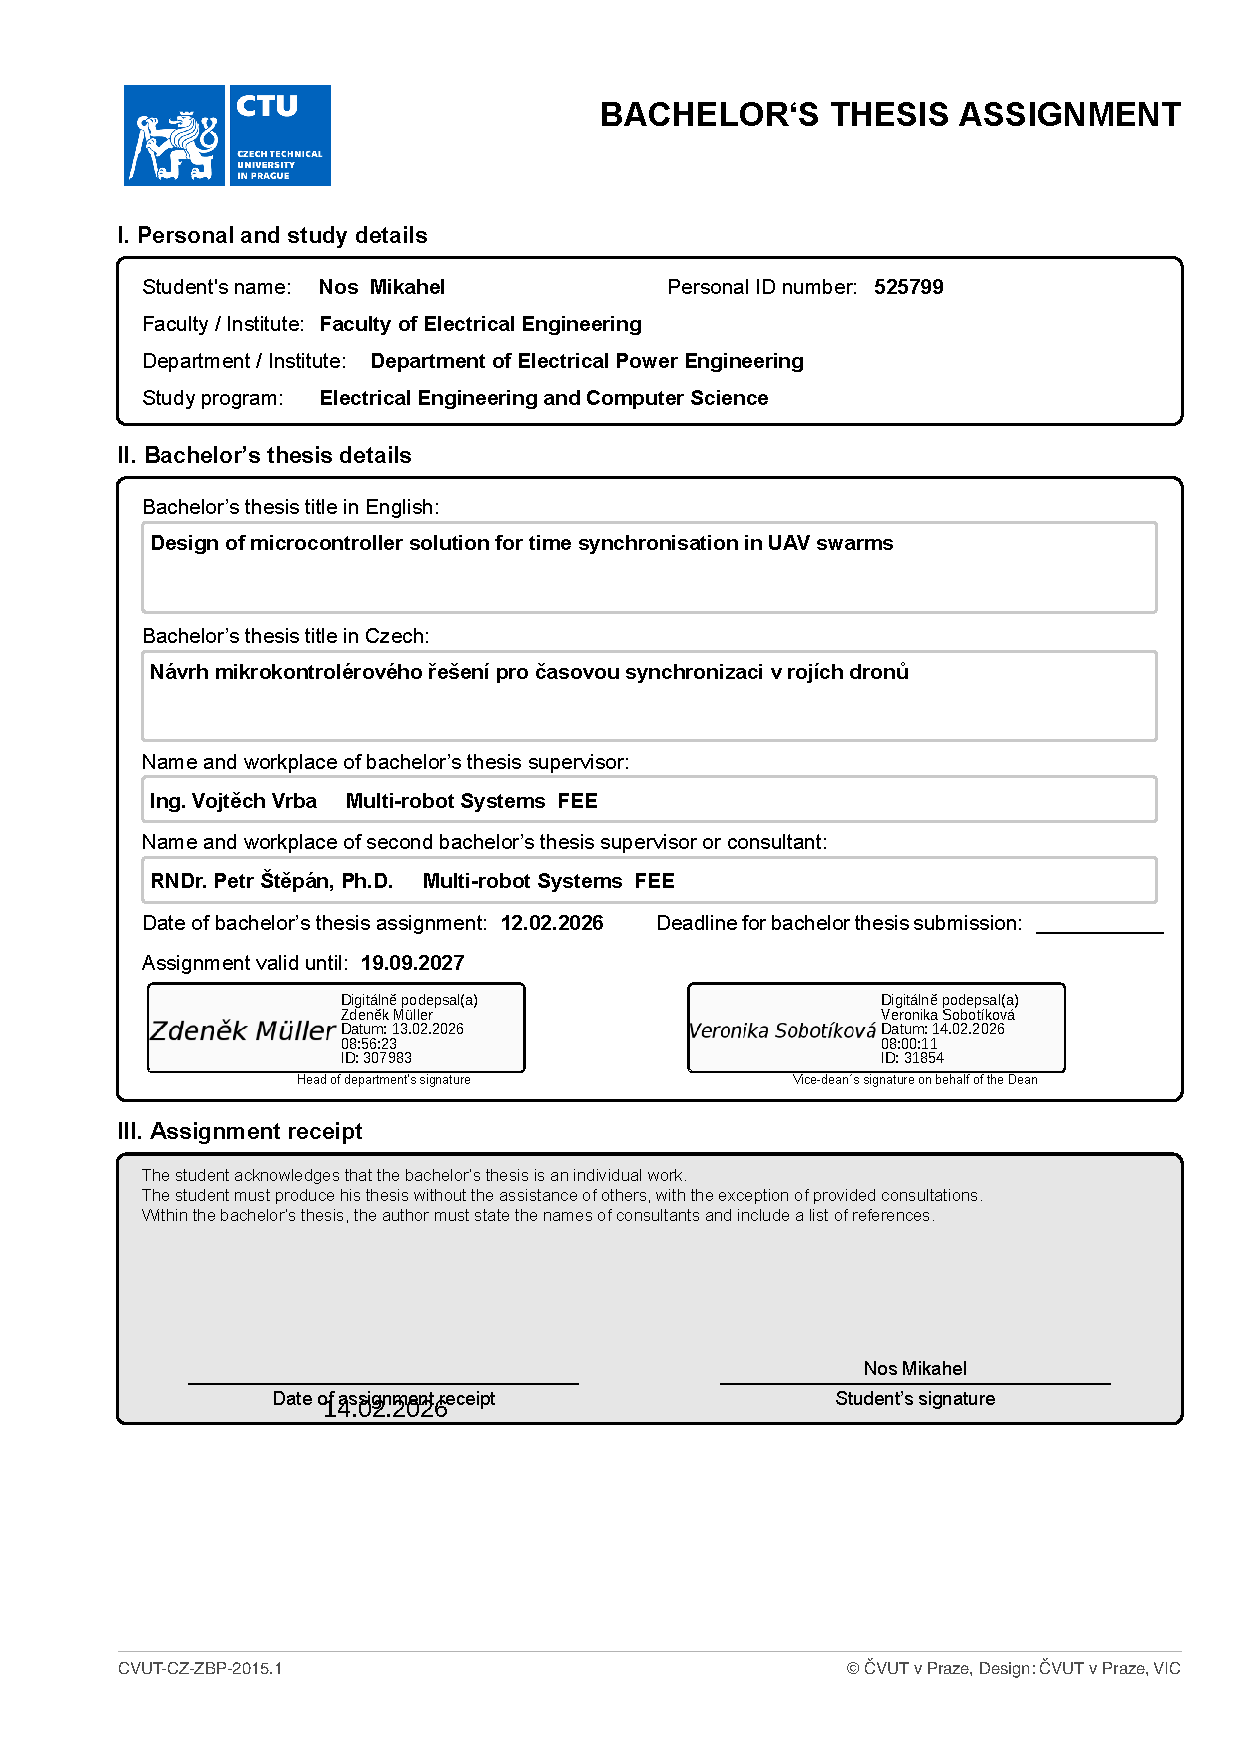
\includepdf{src/assignment.pdf}

%% --------------------------------------------------------------
%% |                         Declaration                        |
%% --------------------------------------------------------------

\conditionalClearPage

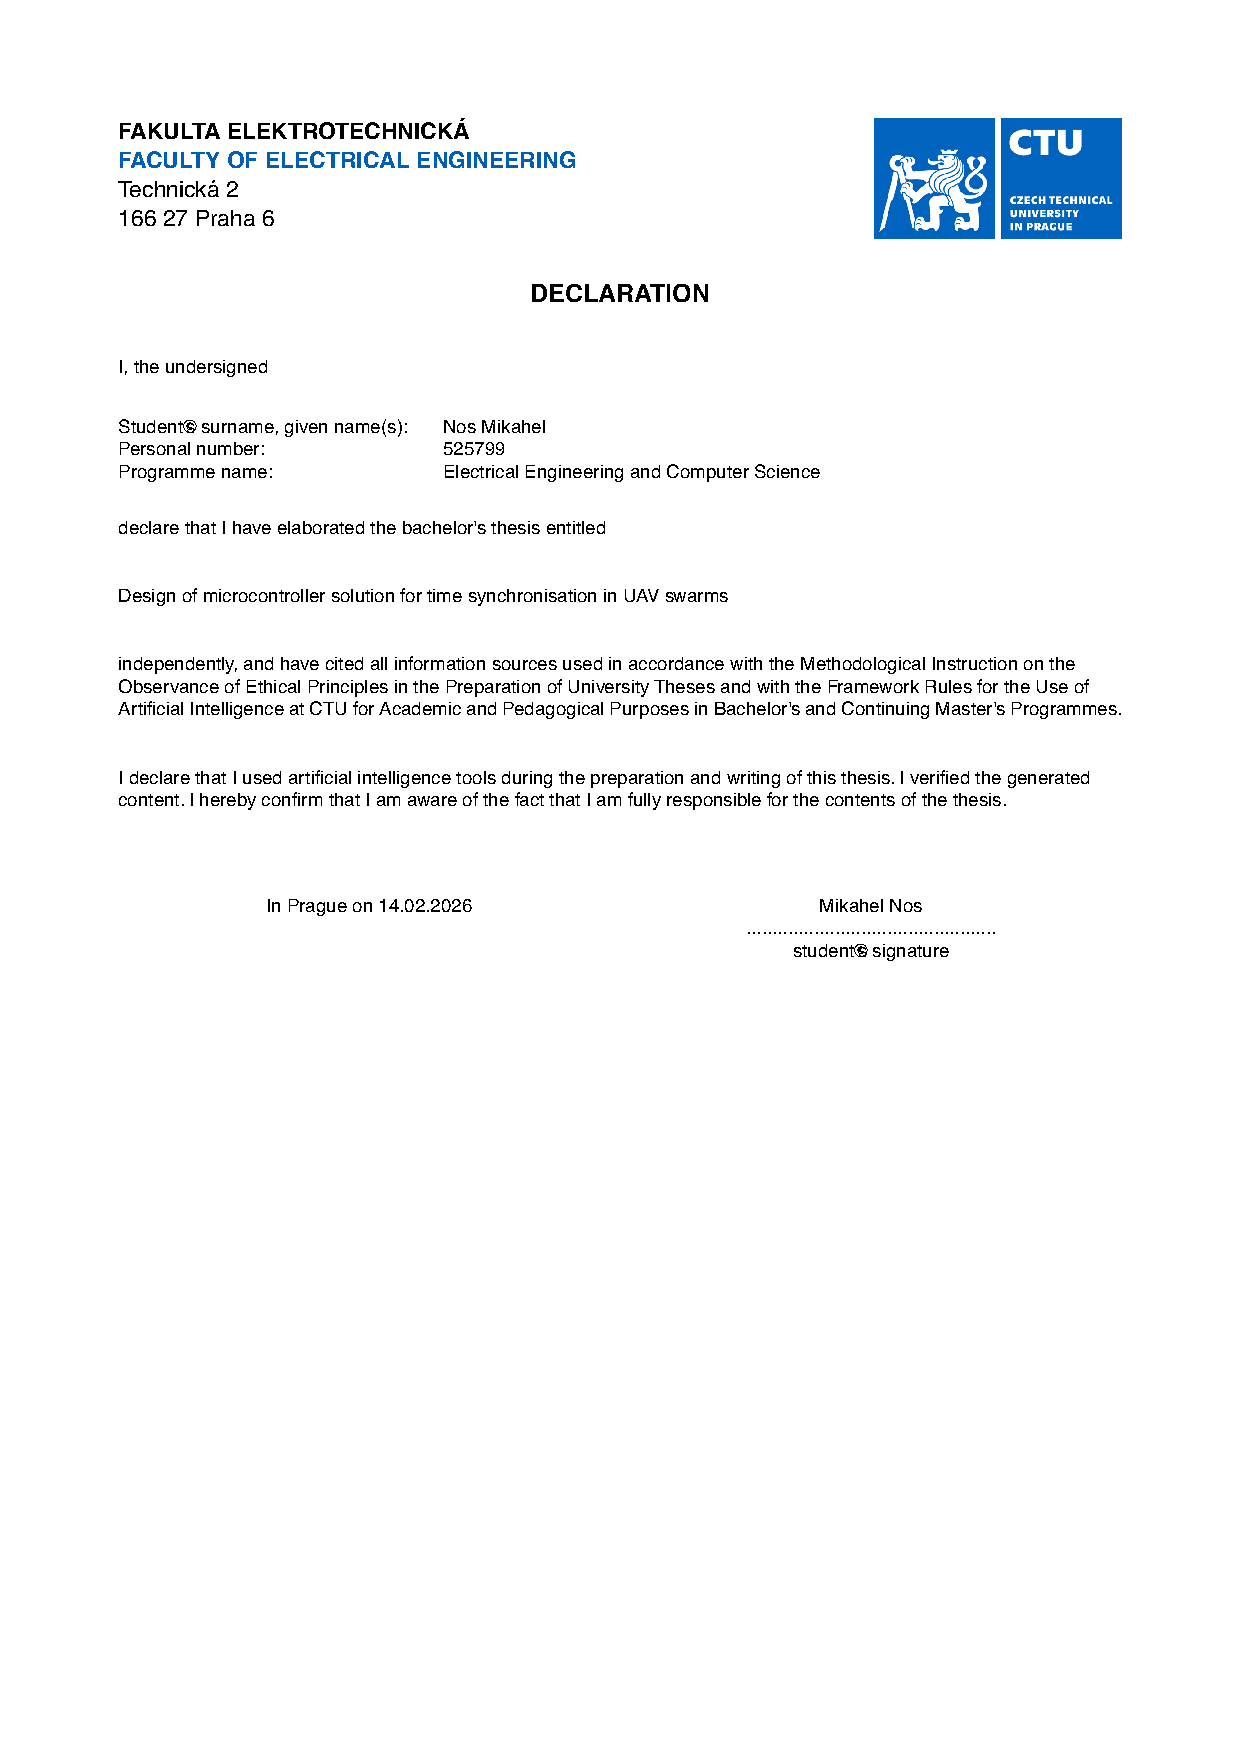
\includepdf{src/declaration.pdf}

%% --------------------------------------------------------------
%% |                          Abstracts                         |
%% --------------------------------------------------------------

\conditionalClearPage

%!TEX root = ../main.tex

\begin{changemargin}{0.8cm}{0.8cm}

~\vfill{}

\section*{Abstract}
\vskip 0.5em

\sloppy
This thesis presents the design, implementation, and evaluation of a microcontroller-based time synchronization prototype intended for UAV swarm-related experiments. The developed system combines DCF77 absolute time reception, RTK PPS-based second generation, STM32 firmware processing, UART diagnostic communication, and ROS2-based logging and analysis.

The hardware implementation is based on a custom STM32F042F6P6 PCB with USB-C power input, 3.3 V regulation, DCF77 and RTK PPS timing inputs, SWD debugging, and UART diagnostic output. Native STM32 USB communication was investigated during development, but the final validated communication path used an external CP2102 USB-UART bridge because it provided more reliable operation.

The firmware decodes and validates DCF77 frames, maintains a software real-time clock, processes RTK PPS interrupt events, and transmits synchronization diagnostics to the companion-computer environment. ROS2 nodes receive the UART messages, publish them to topics, store CSV logs, and support Python-based post-processing.

An additional logic-analyzer-based PPS-to-GPIO measurement showed typical sub-millisecond physical response during normal operation, while occasional latency spikes confirmed that the practical precision is limited mainly by EXTI interrupt latency, HAL processing overhead, and GPIO switching delay.

The final evaluation confirmed stable DCF77-based time acquisition and RTK PPS-driven second generation. In the final RTK PPS test, the measured \texttt{RTK\_DIFF} remained equal to 0 ms for all synchronized samples at millisecond-level measurement resolution, with an estimated drift of 0.000 ms/s. The results do not prove sub-microsecond synchronization accuracy, but they validate a functional synchronization prototype with no observable long-term software-clock drift at the implemented measurement resolution.

\vskip 1em

{\bf Keywords:} \Keywords

\vskip 2.5cm

\end{changemargin}


\conditionalClearPage

%!TEX root = ../main.tex

\begin{changemargin}{0.8cm}{0.8cm}

~\vfill{}

\section*{Abstrakt}
\vskip 0.5em

\sloppy
Tato práce představuje návrh, implementaci a vyhodnocení prototypu časové synchronizace založeného na mikrokontroléru pro budoucí experimenty s roji UAV. Vyvinutý systém kombinuje příjem absolutního času pomocí signálu DCF77, generování sekund podle RTK PPS, firmware pro STM32, diagnostickou komunikaci přes UART a záznam a analýzu dat v prostředí ROS2.

Hardwarová implementace je založena na vlastní desce plošných spojů s mikrokontrolérem STM32F042F6P6, napájením přes USB-C, 3.3 V regulací, vstupy pro DCF77 a RTK PPS, rozhraním SWD pro ladění a diagnostickým výstupem přes UART. Nativní USB komunikace mikrokontroléru STM32 byla během vývoje testována, ale ve finální ověřené verzi byl použit externí převodník CP2102 USB-UART, protože poskytoval spolehlivější komunikaci.

Firmware dekóduje a ověřuje rámce DCF77, udržuje softwarové hodiny reálného času, zpracovává přerušení RTK PPS a odesílá diagnostické zprávy do prostředí companion computeru. Uzly ROS2 přijímají UART zprávy, publikují je do témat, ukládají CSV logy a umožňují následné zpracování pomocí Python skriptů.

Finální vyhodnocení potvrdilo stabilní získávání času z DCF77 a generování sekund řízené signálem RTK PPS. Ve finálním RTK PPS testu zůstala měřená hodnota \texttt{RTK\_DIFF} rovna 0 ms pro všechny synchronizované vzorky při milisekundovém rozlišení měření a odhadovaný drift byl 0.000 ms/s. Výsledky neprokazují submikrosekundovou přesnost synchronizace, ale ověřují funkční synchronizační prototyp bez pozorovatelného dlouhodobého driftu softwarových hodin v dostupném rozlišení měření.
\vskip 1em

{\bf Klíčová slova:} \KlicovaSlova

\vskip 2.5cm

\end{changemargin}


%% --------------------------------------------------------------
%% |                        Abbreviations                       |
%% --------------------------------------------------------------

\conditionalClearPage

\begin{changemargin}{0.8cm}{0.8cm}

~\vfill{}

\section*{Abbreviations}

% this will print only the used abbreviations
%!TEX root = ../main.tex
% \printacronyms
\begin{acronym}
  \acro{AMS}[AMS]{Advanced Monolithic Systems}
  \acro{API}[API]{Application Programming Interface}	
  \acro{BCD}[BCD]{Binary-Coded Decimal}
  \acro{CDC}[CDC]{Communications Device Class}
  \acro{CP2102}[CP2102]{Silicon Labs USB-to-UART bridge}
  \acro{CSV}[CSV]{Comma-Separated Values}
  \acro{CTU}[CTU]{Czech Technical University}
  \acro{DCF77}[DCF77]{German longwave time signal transmitter}
  \acro{DOF}[DOF]{Degree of Freedom}
  \acro{EMC}[EMC]{Electromagnetic Compatibility}
  \acro{EMI}[EMI]{Electromagnetic Interference}
  \acro{ESC}[ESC]{Electronic Speed Controller}
  \acro{EXTI}[EXTI]{External Interrupt/Event Controller}
  \acro{FOV}[FOV]{Field of View}
  \acro{FTSP}[FTSP]{Flooding Time Synchronization Protocol}
  \acro{HAL}[HAL]{Hardware Abstraction Layer}
  \acro{HSI}[HSI]{High-Speed Internal oscillator}
  \acro{GNSS}[GNSS]{Global Navigation Satellite System}
  \acro{GPIO}[GPIO]{General-Purpose Input/Output}
  \acro{GPS}[GPS]{Global Positioning System}
  \acro{IMU}[IMU]{Inertial Measurement Unit}
  \acro{ISR}[ISR]{Interrupt Service Routine}
  \acro{LDO}[LDO]{Low-Dropout Regulator}
  \acro{LiDAR}[LiDAR]{Light Detection and Ranging}
  \acro{LKF}[LKF]{Linear Kalman Filter}
  \acro{LTI}[LTI]{Linear Time-Invariant}
  \acro{MAV}[MAV]{Micro Aerial Vehicle}
  \acro{MCU}[MCU]{Microcontroller Unit}
  \acro{MPC}[MPC]{Model Predictive Control}
  \acro{MRS}[MRS]{Multi-Robot Systems Group}
  \acro{NMEA}[NMEA]{National Marine Electronics Association}
  \acro{PCB}[PCB]{Printed Circuit Board}
  \acro{PLL}[PLL]{Phase-Locked Loop}
  \acro{PPS}[PPS]{Pulse Per Second}
  \acro{PTP}[PTP]{Precision Time Protocol}
  \acro{RC}[RC]{Resistor-Capacitor}
  \acro{ROS}[ROS]{Robot Operating System}
  \acro{ROS2}[ROS2]{Robot Operating System 2}
  \acro{RTC}[RTC]{Real-Time Clock}
  \acro{RTK}[RTK]{Real-Time Kinematic}
  \acro{SLAM}[SLAM]{Simultaneous Localization and Mapping}
  \acro{STM32}[STM32]{STMicroelectronics 32-bit microcontroller family}
  \acro{SWD}[SWD]{Serial Wire Debug}
  \acro{TIM}[TIM]{Timer Peripheral}
  \acro{UART}[UART]{Universal Asynchronous Receiver-Transmitter}
  \acro{UAV}[UAV]{Unmanned Aerial Vehicle}
  \acro{UGV}[UGV]{Unmanned Ground Vehicle}
  \acro{UKF}[UKF]{Unscented Kalman Filter}
  \acro{USB}[USB]{Universal Serial Bus}
  \acro{UTC}[UTC]{Coordinated Universal Time}
  \acro{WSL}[WSL]{Windows Subsystem for Linux}
\end{acronym}

\vskip 2.5cm

\end{changemargin}

\conditionalClearPage

%% --------------------------------------------------------------
%% |                      Table of contents                     |
%% --------------------------------------------------------------

\tableofcontents

\conditionalClearPage

% set up the full page style with normal page numbering
\pagestyle{full}
\pagenumbering{arabic}

%% --------------------------------------------------------------
%% |                        introduction                        |
%% --------------------------------------------------------------

%!TEX root = ../main.tex

\chapter{Introduction\label{chap:introduction}}
Precise time synchronization is an important requirement in distributed UAV systems, where sensor data, control actions, and diagnostic messages must be aligned across multiple nodes. \cite{r1,r2,r7} This thesis focuses on the design and validation of a compact STM32-based synchronization module that combines DCF77 absolute time reception with RTK PPS-based second generation and ROS2-based evaluation.

The chapter introduces the motivation for the work, defines the main objectives, and summarizes the structure of the thesis.

\section{Motivation}

The increasing use of UAV swarms in applications such as cooperative mapping, formation flight, and distributed sensing places high demands on consistent timing between individual nodes. \cite{r1,r2,r7} In such systems, sensor measurements, control actions, and diagnostic messages must be timestamped in a comparable time base so that data from multiple vehicles can be correctly correlated.

Many synchronization approaches rely on communication networks or external computing resources. However, wireless communication in UAV systems can introduce variable latency, packet delay, and jitter, especially in dynamic multi-robot environments. \cite{lopez2021uavmesh} These effects make purely network-based synchronization unsuitable as the only timing source when deterministic timing behavior is required.

This thesis is motivated by the need for a compact embedded synchronization module that can provide reliable local time information independently of network delay. The developed solution uses a DCF77 radio time signal to obtain absolute calendar time and an RTK receiver PPS signal to generate a stable one-second reference. An STM32 microcontroller decodes and validates the time information, maintains a software clock, and transmits synchronization diagnostics to a ROS2-based evaluation environment.

The goal is therefore not only to design a theoretical synchronization concept, but also to implement and experimentally validate a practical hardware and firmware pipeline suitable for future UAV swarm timing experiments.

\section{Objectives}

The main objective of this thesis is to design, implement, and evaluate a microcontroller-based time synchronization module for UAV swarm-related experiments. The work focuses on creating a compact embedded system capable of acquiring absolute time, maintaining a local software clock, and validating synchronization behavior through a ROS2-based evaluation pipeline.
\\
The specific objectives are:
\begin{itemize}
    \item to analyze time synchronization principles relevant to distributed UAV and multi-robot systems,
    \item to design a custom STM32-based hardware platform with interfaces for DCF77, RTK PPS, UART communication, and debugging,
    \item to implement firmware for DCF77 frame decoding, parity validation, software clock maintenance, and RTK PPS-driven second generation,
    \item to integrate the synchronization module with a companion-computer environment using UART and ROS2,
    \item to experimentally evaluate synchronization stability, communication reliability, and timing behavior using logged measurement data.
\end{itemize}

The main contribution of this thesis is the design and validation of a complete embedded synchronization prototype. The work includes the custom STM32-based PCB, firmware for DCF77 decoding and RTK PPS-driven clock generation, UART diagnostic communication, and a ROS2-based logging and analysis pipeline. The validated result is stable DCF77-based absolute time acquisition and PPS-driven second generation with no observable long-term software-clock drift at millisecond-level measurement resolution. The work does not claim sub-microsecond synchronization accuracy, because the final evaluation was performed using firmware diagnostics, UART messages, ROS2 logs, and Python post-processing rather than direct hardware-level timestamping.

\section{Structure of the Thesis}

The thesis is structured into eight chapters. Chapter 1 introduces the motivation, objectives, and scope of the work. Chapter 2 presents the theoretical background of time synchronization, clock drift, GNSS/RTK timing, DCF77 time reception, and microcontroller-based timing architectures. Chapter 3 describes the overall system design and explains the role of the main synchronization components.

Chapter 4 focuses on the hardware implementation of the custom STM32-based PCB, including the power supply, signal interfaces, PCB layout, and communication paths. Chapter 5 describes the firmware implementation, including DCF77 decoding, parity validation, software clock maintenance, RTK PPS-based second generation, and UART diagnostic output.

Chapter 6 presents the integration of the synchronization module with the ROS2 environment used for data collection and analysis. Chapter 7 describes the measurement setup, logged results, synchronization behavior, and practical limitations of the evaluation method. Finally, Chapter 8 summarizes the achieved results and outlines possible directions for future improvements.


%% --------------------------------------------------------------
%% |                        Theoretical Background                        |
%% --------------------------------------------------------------

%!TEX root = ../main.tex

\chapter{Theoretical Background\label{chap:theoreticalBackground}}

This chapter presents the theoretical principles required to understand the design of the proposed time-synchronization system. It first explains clock offset, clock drift, oscillator stability, and the difference between synchronization accuracy and precision in distributed embedded systems \cite{kopetz2011realtime,lamport1978time,allan1966statistics,levine2012atomic}. It then discusses common synchronization approaches, including network-based methods such as IEEE 1588 PTP and hardware-assisted synchronization using external timing signals \cite{ieee1588,maroti2004ftsp,cristian1989probabilistic}.

The chapter also introduces the two external timing references used in this work. DCF77 is discussed as a longwave radio time signal that provides absolute calendar time \cite{ptbDcf77}, while GNSS/RTK PPS is discussed as a stable one-second timing reference suitable for disciplining a local embedded clock \cite{r6}. Finally, the chapter explains microcontroller timing architectures, including hardware timers, external interrupts, and interrupt-driven timestamping, which form the basis of the STM32 firmware implementation.

\section{Time Synchronization Principles}

Time synchronization in distributed systems is the process of aligning independent local clocks to a common time reference. In a UAV swarm, each vehicle or embedded module contains its own oscillator-driven clock, and these clocks do not remain identical over time. Manufacturing tolerances, temperature changes, supply-voltage variation, and oscillator aging cause local clocks to drift from one another \cite{kopetz2011realtime,allan1966statistics,levine2012atomic}.

In distributed robotic systems, inconsistent time bases can lead to incorrect ordering of events, inaccurate sensor-data correlation, and degraded coordination between agents. This is especially relevant for UAV swarms, where measurements from inertial sensors, cameras, GNSS receivers, and communication messages may need to be compared across multiple platforms \cite{r1,r2,r7}. The general problem of ordering events in distributed systems was formalized by Lamport, who showed that independent nodes cannot assume a globally consistent event order without a synchronization mechanism \cite{lamport1978time}.

Synchronization methods can be divided into two broad categories. Network-based methods estimate clock offset by exchanging timestamped messages between nodes, as in Cristian's algorithm, FTSP, or IEEE 1588 PTP \cite{cristian1989probabilistic,maroti2004ftsp,ieee1588}. These methods are flexible, but their precision depends on communication-delay stability. In wireless UAV networks, variable latency, interference, and packet buffering can introduce significant jitter \cite{lopez2021uavmesh}.

\subsection{Clock Model in Distributed Systems}

A local clock in a distributed embedded system can be described as an approximation of an ideal reference time. If $t$ denotes the true reference time, the clock of node $i$ can be modeled as
\begin{equation}
C_i(t) = \alpha_i t + \beta_i ,
\end{equation}
where $C_i(t)$ is the local clock value, $\alpha_i$ represents the clock skew, and $\beta_i$ represents the clock offset \cite{kopetz2011realtime,lamport1978time}. The offset describes the instantaneous time difference between the local clock and the reference time, while the skew describes the relative frequency error of the oscillator.

If two nodes have different skew values, their clocks diverge even if they are initially synchronized. For example, an oscillator error of 10 ppm means that the clock can drift by approximately $10~\mu$s every second. Over longer operation, this error accumulates and can reach milliseconds or seconds if no external correction is applied \cite{allan1966statistics,levine2012atomic}.

This clock model is directly relevant to the implemented synchronization module. The STM32 timer provides the local time base, but its oscillator is not sufficiently accurate for long-term independent operation. Therefore, the firmware periodically corrects the local software clock using external timing references. In the final implementation, DCF77 provides absolute calendar time, while the RTK PPS signal provides a stable one-second boundary used to prevent accumulated drift.

\subsection{Oscillator Stability and Drift}

The accuracy of a local embedded clock depends mainly on the stability of its oscillator. Microcontrollers commonly use internal RC oscillators or external crystal oscillators as their clock source. These oscillators are not ideal and their frequency can deviate from the nominal value because of manufacturing tolerance, temperature variation, supply-voltage changes, aging, and mechanical stress \cite{allan1966statistics,levine2012atomic}.

Oscillator frequency error is commonly expressed in parts per million (ppm). A frequency error of 1 ppm corresponds to a timing error of approximately $1~\mu$s per second. Therefore, a 10 ppm oscillator can accumulate about $10~\mu$s of error every second, which corresponds to approximately 36 ms after one hour if the clock is not corrected.

This accumulated error is called clock drift. In short-duration measurements, drift may be small, but in long-running distributed systems it becomes significant. For UAV swarm applications, such drift can reduce the consistency of sensor timestamps and make comparison of events between different nodes unreliable \cite{kopetz2011realtime}.

The implemented system addresses this problem by not relying only on the free-running STM32 oscillator. DCF77 is used to obtain absolute time information, and the RTK PPS signal is used as an external one-second reference. By incrementing the software clock from PPS events after synchronization, the final firmware prevents long-term drift of the internal software clock.

\subsection{Precision and Accuracy}

In time synchronization, precision and accuracy describe different properties and should not be used interchangeably. Accuracy expresses how close a local clock is to an absolute reference time, such as UTC. Precision expresses how closely multiple clocks agree with each other, regardless of whether they are perfectly aligned to absolute time \cite{kopetz2011realtime}.

For example, two UAV nodes may have high relative precision if their clocks differ only by a few microseconds, even if both clocks are shifted from UTC by several milliseconds. Conversely, a single node may be accurate with respect to UTC, but poor communication or local timestamping delays may reduce the precision of synchronization between multiple nodes.

In distributed UAV systems, both properties are important. Absolute accuracy is required when measurements must be related to a global time scale, while relative precision is important when comparing sensor data or events between multiple vehicles \cite{r1,r2,r7}. In this thesis, DCF77 is used to provide absolute calendar time \cite{ptbDcf77}, while the RTK PPS signal is used to provide a stable one-second reference for maintaining the local software clock.

The experimental evaluation in this work combines firmware/ROS2-based measurements with a logic-analyzer-based PPS-to-GPIO measurement. The firmware and ROS2 logs provide millisecond-level visibility into software-clock behavior and communication timing, while the logic-analyzer measurement provides a practical estimate of the physical response delay of the implemented interrupt-based synchronization path.

\subsection{Network-Based Synchronization Methods}

Network-based synchronization methods align clocks by exchanging timestamped messages between nodes. A node estimates the time offset between its local clock and another clock by measuring message transmission and reception times. Classical examples include Cristian's algorithm, the Flooding Time Synchronization Protocol (FTSP), and the IEEE 1588 Precision Time Protocol (PTP) \cite{cristian1989probabilistic,maroti2004ftsp,ieee1588}.

The main limitation of these methods is their dependence on communication-delay estimation. If the network delay is constant and symmetric, the clock offset can be estimated accurately. However, if the delay varies, the synchronization error increases. A simplified relation is
\begin{equation}
\varepsilon \approx \frac{\sigma_{delay}}{2},
\end{equation}
where $\varepsilon$ is the synchronization uncertainty and $\sigma_{delay}$ represents delay variability.

In wired networks, protocols such as IEEE 1588 PTP can achieve high precision, especially when hardware timestamping is available \cite{ieee1588}. In wireless UAV networks, however, message delay can vary because of medium access contention, interference, packet buffering, retransmissions, and changing topology \cite{lopez2021uavmesh}. This makes purely network-based synchronization less suitable as the primary timing mechanism for deterministic embedded synchronization.

For this reason, the synchronization approach used in this thesis does not depend on ROS2 message arrival time or wireless communication latency. Instead, timing is generated locally on the STM32 using external physical references. DCF77 provides absolute time information, and the RTK PPS signal provides a stable second boundary. ROS2 is used only for logging, monitoring, and evaluation of the produced synchronization data.

\subsection{Hardware-Assisted Synchronization}

Hardware-assisted synchronization uses a physical timing signal to align local clocks. Instead of estimating time offset through network message exchange, an external signal is connected directly to embedded hardware, where it can be detected with low and predictable latency. Examples of such timing signals include PPS outputs from GNSS receivers and radio time signals such as DCF77 \cite{ptbDcf77}.

A major advantage of hardware-assisted synchronization is that the timing reference is separated from communication latency. When a PPS edge is captured by a microcontroller timer or external interrupt, the synchronization event is generated locally and does not depend on packet transmission, operating-system scheduling, or ROS2 message arrival time. This reduces the uncertainty caused by variable communication delay \cite{kopetz2011realtime}.

The synchronization uncertainty can be expressed as a combination of physical and embedded timing errors:
\begin{equation}
\varepsilon_{sync} \approx \varepsilon_{source} + \varepsilon_{capture} + \varepsilon_{jitter},
\end{equation}
where $\varepsilon_{source}$ represents the timing error of the external reference, $\varepsilon_{capture}$ represents the timer or interrupt capture uncertainty, and $\varepsilon_{jitter}$ represents remaining implementation-related jitter.

The system developed in this thesis follows this approach. DCF77 is used to decode absolute calendar time, while the RTK PPS signal is used as the stable one-second event for the STM32 software clock. After the first valid DCF77 synchronization, the firmware increments the internal clock using RTK PPS interrupts. This prevents long-term software-clock drift and keeps synchronization independent of ROS2 transport timing.

\subsection{Theoretical Limitations}

Even when hardware-assisted synchronization is used, perfect time alignment cannot be achieved in practice. The final synchronization quality is limited by both the external timing source and the embedded implementation. Important error sources include reference-signal jitter, timer resolution, interrupt latency, input threshold uncertainty, oscillator instability between reference events, and electrical noise on the PCB \cite{kopetz2011realtime,allan1966statistics,levine2012atomic}.

The timer resolution creates a fundamental quantization limit. If a timer runs at frequency $f_{clk}$, the smallest directly measurable time step is
\begin{equation}
\Delta t = \frac{1}{f_{clk}} .
\end{equation}
Any event detected by the microcontroller can only be represented with this finite resolution unless additional interpolation or specialized hardware timestamping is used.

In addition to timer resolution, interrupt processing can introduce jitter. Although hardware timer capture can store an event timestamp independently of software execution, interrupt-based firmware still requires careful design to avoid delays caused by long interrupt routines, lower-priority tasks, or communication handling \cite{kopetz2011realtime}. For this reason, time-critical processing should be kept short and separated from non-critical communication tasks.

In the implemented system, part of the synchronization behavior was evaluated using UART messages, firmware counters, and ROS2 logs. This measurement path provides millisecond-level visibility and is sufficient to verify stable PPS-driven second generation and elimination of long-term software-clock drift. In addition, a logic-analyzer-based hardware measurement was later used to estimate the physical offset between the RTK PPS input and an STM32-generated synchronization GPIO output. This additional measurement provided direct insight into the practical PPS-to-firmware response delay, but the observed precision remained limited by interrupt latency, GPIO switching delay, HAL overhead, and firmware execution jitter.

\section{GNSS and RTK Fundamentals}

Global Navigation Satellite Systems (GNSS) provide positioning and timing information by receiving precisely time-stamped signals from satellites. Since satellite navigation systems depend on accurate time measurement, GNSS receivers can also be used as stable timing sources in embedded and robotic systems \cite{teunissen2017springer}.

Real-Time Kinematic (RTK) GNSS improves positioning accuracy by using correction data from a reference station. Although RTK is mainly used for centimeter-level positioning, RTK-capable receivers commonly provide a precise PPS output that can be used as an external timing reference. In this thesis, the RTK receiver is therefore important primarily as a source of a stable one-second PPS signal, not as a fully decoded GNSS time source.

The developed system combines this PPS reference with DCF77 absolute time reception. DCF77 provides calendar time, while the RTK PPS signal provides a stable second boundary for the STM32 software clock. This separation allows the firmware to maintain absolute time while reducing long-term drift of the local embedded clock.

\subsection{GNSS Time Reference}

GNSS receivers determine position and time by measuring signals transmitted from navigation satellites. Since each satellite signal is associated with a precise transmission time, GNSS systems rely on accurate timekeeping as a fundamental part of their operation \cite{teunissen2017springer}. As a result, GNSS receivers can provide not only position information, but also useful timing outputs for embedded systems.

A common timing output of GNSS receivers is the Pulse Per Second (PPS) signal. The PPS signal produces one electrical pulse per second, with the active edge aligned to the receiver's internal estimate of GNSS time. When satellite reception is stable, this pulse can be used as an external reference for disciplining a local microcontroller clock.

In the implemented system, the GNSS/RTK receiver was used primarily through its PPS output. The firmware did not fully decode GNSS time messages for calendar-time acquisition. Instead, absolute time was obtained from the DCF77 signal, while the RTK PPS signal was used to generate stable one-second increments of the STM32 software clock. This separation reflects the final practical architecture of the project.

\subsection{Real-Time Kinematic (RTK) Enhancement}

Real-Time Kinematic (RTK) is a GNSS enhancement technique that improves positioning accuracy by using correction data from a reference station with known coordinates. In contrast to standard code-based GNSS positioning, RTK uses carrier-phase measurements and ambiguity resolution to achieve significantly higher positioning accuracy \cite{teunissen2017springer}.

In UAV systems, RTK is commonly used when accurate position estimation is required for navigation, mapping, formation flight, or multi-robot localization. High-quality GNSS and RTK solutions can improve spatial consistency between vehicles and support more reliable coordination in outdoor environments \cite{r6}.

In this thesis, RTK is not used as a fully processed positioning pipeline inside the STM32 firmware. The microcontroller does not compute RTK corrections or decode full GNSS time messages. Instead, the RTK-capable receiver is used mainly as a source of a stable PPS signal. This PPS signal provides a precise one-second timing event that is used to drive the local STM32 software clock after DCF77-based absolute time synchronization.

This distinction is important for the final system architecture. DCF77 provides the absolute calendar time, while the RTK PPS signal improves the stability of second generation. Therefore, RTK contributes to the timing pipeline through its hardware PPS output rather than through full RTK data processing in the microcontroller.

\subsection{Timing Accuracy and Error Sources}

GNSS-based timing can provide a highly stable external time reference, but its practical accuracy depends on both satellite-signal conditions and receiver implementation. Important GNSS error sources include satellite clock and ephemeris errors, ionospheric and tropospheric delays, multipath reflections, receiver noise, and antenna placement \cite{teunissen2017springer}. These effects influence the receiver solution and can also affect the stability of the generated PPS signal.

When the PPS signal is used in an embedded system, additional implementation-related errors appear. These include propagation delay in cables and PCB traces, input threshold uncertainty at the microcontroller pin, timer quantization, interrupt latency, and software processing jitter \cite{kopetz2011realtime}. Therefore, the total timing uncertainty is not determined only by the GNSS receiver, but by the complete signal path from the receiver output to the firmware measurement.

The total uncertainty can be described conceptually as
\begin{equation}
\varepsilon_{total} \approx \varepsilon_{gnss} + \varepsilon_{pps} + \varepsilon_{hardware} + \varepsilon_{software},
\end{equation}
where $\varepsilon_{gnss}$ represents GNSS-related timing errors, $\varepsilon_{pps}$ represents receiver PPS output jitter, $\varepsilon_{hardware}$ represents signal-routing and timer-capture limitations, and $\varepsilon_{software}$ represents firmware and logging uncertainty.

In the implemented system, the RTK PPS signal was used as the external reference for stable second generation. Firmware and ROS2 evaluation confirmed that the internal software clock remained aligned with the PPS event at millisecond-level measurement resolution. In addition, a logic-analyzer measurement was used to observe the physical PPS-to-GPIO synchronization delay. This measurement provided practical hardware-level validation of the implemented response time, but it still did not quantify the absolute nanosecond-level accuracy of the RTK PPS source itself. A more precise internal synchronization architecture would require timer input capture or dedicated hardware timestamping.

\subsection{Suitability for UAV Swarms}

UAV swarms require consistent timing because measurements and actions from multiple vehicles often need to be compared or coordinated. Applications such as cooperative mapping, formation flight, distributed sensing, and multi-robot localization depend on reliable timestamping and event ordering across different platforms \cite{r1,r2,r7}.

A suitable synchronization approach for UAV swarms should be scalable and should not rely only on communication between vehicles. Wireless networks in UAV systems can experience changing latency, packet loss, interference, and dynamic topology changes, which makes network-based synchronization less deterministic \cite{lopez2021uavmesh}. For this reason, an external timing reference available independently to each node is attractive.

GNSS-based timing is suitable for outdoor UAV systems because each vehicle can receive a common global reference without exchanging synchronization messages with other vehicles \cite{teunissen2017springer}. In practical embedded implementations, the PPS output of a GNSS or RTK receiver can be connected directly to a microcontroller input and used as a stable second-boundary reference.

The system developed in this thesis follows this idea, but with a practical separation of roles. DCF77 is used to obtain absolute calendar time, while the RTK PPS signal is used to stabilize the local STM32 software clock. This architecture is suitable as a prototype for UAV swarm timing experiments because it reduces dependence on ROS2 or wireless message timing and allows synchronization behavior to be logged and evaluated through the companion-computer environment.

\section{Microcontroller Timing Architectures}

Microcontrollers are suitable for embedded time-synchronization systems because they include hardware peripherals for deterministic event detection and time measurement. Typical timing-related peripherals include clock sources, prescalers, hardware timers, external interrupt lines, capture/compare units, and communication interfaces \cite{kopetz2011realtime}. These components allow a microcontroller to measure external timing signals and maintain a local time base with limited software overhead.

In synchronization applications, the microcontroller clock defines the resolution of internal time measurements, while external signals provide correction or reference events. A timer can be configured as a free-running counter, and signal edges can be detected using external interrupts or hardware input-capture functionality. This makes it possible to measure pulse widths, detect periodic timing events, and update a software clock.

The implemented system uses these principles on an STM32F042 microcontroller. TIM2 is used as the main timing counter for signal measurements, external interrupt lines are used to detect DCF77 and RTK PPS signal edges, and firmware logic maintains a software real-time clock. After a valid DCF77 frame provides absolute time, the RTK PPS interrupt is used to generate stable one-second increments. UART communication is used only for diagnostics and ROS2 logging, not as the primary timing reference.

\subsection{Internal Clock Sources}

A microcontroller requires a clock source to execute instructions and drive peripheral timing. Common clock sources include internal RC oscillators, external crystal oscillators, low-speed oscillators for real-time clocks, and phase-locked loops used for frequency multiplication. The STM32F042 family supports several clock options, including an internal 8 MHz RC oscillator, an internal 48 MHz oscillator, external crystal sources, and PLL-based clock generation \cite{stm32F042Datasheet,stm32F0ReferenceManual}.

The choice of clock source influences timer resolution, power consumption, peripheral availability, and long-term timing stability. Internal RC oscillators are simple and require no external components, but their frequency accuracy is lower than that of external crystal oscillators. External crystals usually provide better stability, while PLLs can generate higher system frequencies but add configuration complexity.

In the final implementation of this thesis, the STM32 firmware used the internal HSI clock configuration because it provided stable operation during development and testing. Earlier attempts to use the native USB clock path and HSI48 oscillator were not reliable on the prototype hardware. Therefore, the final communication path used UART through an external CP2102 USB-UART bridge, while timing was stabilized using external synchronization signals.

The internal STM32 clock was not treated as an absolute long-term time reference. Instead, it provided the local timing base for firmware execution and signal measurement. Absolute time was obtained from DCF77, and long-term second generation was stabilized by the RTK PPS signal.

\subsection{Hardware Timers and Counters}

Hardware timers are microcontroller peripherals used to measure time intervals, generate periodic events, and timestamp external signals. A timer usually consists of a counter register, a prescaler, an auto-reload value, and optional capture/compare channels. The counter is incremented by a clock derived from the microcontroller clock tree \cite{stm32F0ReferenceManual}.

If the timer input clock is $f_{clk}$ and the prescaler value is $PSC$, the effective timer counting frequency is
\begin{equation}
f_{timer} = \frac{f_{clk}}{PSC + 1}.
\end{equation}
The corresponding timer resolution is
\begin{equation}
\Delta t = \frac{1}{f_{timer}}.
\end{equation}
This means that a higher timer frequency gives better timing resolution, but may also require more careful handling of counter overflow and interrupt timing.

In the implemented firmware, TIM2 was configured as the main free-running timing counter. With the STM32 internal clock running at 8 MHz and the TIM2 prescaler set to $8000 - 1$, the effective timer resolution was approximately 1 ms. This resolution was sufficient for measuring DCF77 pulse widths, where logical values are represented by pulse lengths of approximately 100 ms and 200 ms.

The timer was also used for internal software-clock fallback behavior and timing diagnostics. However, the final stable second generation was not based only on the free-running timer. After a valid DCF77 synchronization, the RTK PPS interrupt became the main event used to increment the software clock, preventing long-term drift caused by local timer inaccuracy.

\subsection{Input Capture for PPS Synchronization}

Input capture is a timer function that records the current counter value when an external signal edge is detected. For PPS-based synchronization, the rising edge of the PPS signal can be connected to a timer input channel. When the edge occurs, the hardware stores the timer value in a capture register without waiting for software execution \cite{stm32F0ReferenceManual}.

If $T_k$ is the captured timer value at the $k$-th PPS edge, the firmware can compare it with the expected timer value for an ideal one-second interval. The timing error can be expressed as
\begin{equation}
\varepsilon_k = T_k - T_{expected}.
\end{equation}
This method is useful because the timestamp is created by hardware, so the measurement is less affected by interrupt latency. The interrupt service routine can then process the already captured value later, without changing the original event timestamp \cite{kopetz2011realtime}.

In the final prototype, the RTK PPS signal was detected using an external interrupt input rather than full timer input-capture mode. The interrupt was used to increment the software clock after a valid DCF77 synchronization. This implementation was sufficient to verify PPS-driven second generation and removal of long-term software-clock drift at millisecond-level measurement resolution. For future microsecond-level evaluation, the PPS signal should be connected to a timer input-capture channel and measured using hardware timestamps.

\subsection{Interrupt Latency and Jitter}

Interrupts allow a microcontroller to react to external events without continuously polling an input pin. When an external signal edge occurs, the interrupt controller suspends the current program flow and executes the corresponding interrupt service routine. However, this reaction is not instantaneous. The delay between the physical event and the start of interrupt processing is called interrupt latency \cite{kopetz2011realtime,stm32F0ReferenceManual}.

Interrupt latency depends on several factors, including processor state, interrupt priority, disabled interrupt sections, memory access time, and whether another interrupt is already being processed. If this delay varies between events, the variation is called jitter. In timing-sensitive applications, jitter is important because it can cause uncertainty in measured pulse widths or event timestamps.

This distinction is important for the physical synchronization measurement performed later in this thesis. When the RTK PPS edge triggers an EXTI interrupt and the firmware toggles a GPIO output, the measured PPS-to-GPIO delay does not represent only the external PPS accuracy. It also includes MCU interrupt latency, HAL processing overhead, GPIO switching delay, and any short-term firmware execution jitter.

In general, firmware for time synchronization should keep interrupt service routines short and deterministic. Time-critical operations should be performed immediately, while longer tasks such as message formatting, UART transmission, logging, or complex validation should be deferred to the main loop. This reduces the probability that communication tasks disturb timing measurements \cite{kopetz2011realtime}.

The implemented firmware follows this principle. DCF77 signal edges and RTK PPS events are detected in external interrupt callbacks, while UART diagnostic transmission is performed later in the main loop using a pending flag. This design keeps the interrupt path shorter and helps separate synchronization events from non-time-critical communication with the ROS2 logging system.

\subsection{Clock Discipline and Local Time Base}

Clock discipline is the process of correcting a local clock using an external timing reference. Instead of allowing the local oscillator to run freely, the system periodically compares the local time base with a reference signal and applies corrections to keep the clock error bounded \cite{kopetz2011realtime}.

A local clock can be described as $C(t)$, while the external reference time can be described as $R(t)$. The synchronization objective is to minimize the difference between them:
\begin{equation}
\varepsilon(t) = C(t) - R(t).
\end{equation}
If no correction is applied, oscillator skew causes $\varepsilon(t)$ to grow over time. A disciplined clock reduces this growth by applying periodic corrections based on external synchronization events.

In embedded systems, clock discipline can be implemented in different ways. Some systems adjust oscillator frequency or timer parameters, while simpler implementations maintain a software time base and correct its counters when a reference event is received. The second approach is suitable for compact microcontroller systems where simplicity and deterministic behavior are important.

The implemented firmware uses a software real-time clock containing seconds, minutes, hours, day, month, and year. After a valid DCF77 frame is decoded, the software clock is initialized to the received absolute time. After this initial synchronization, the RTK PPS interrupt is used as the stable one-second event. Each valid PPS event increments the software clock by one second, which prevents accumulated drift from the free-running STM32 timer.

This design separates the local time base from communication timing. UART and ROS2 are used to transmit and evaluate synchronization messages, but they do not discipline the clock directly.

\subsection{Hardware Constraints in UAV Platforms}

UAV platforms impose several practical constraints on embedded synchronization hardware. The module must be compact, lightweight, and power-efficient so that it can be integrated without significantly affecting the vehicle payload, flight time, or internal electronics layout \cite{r2,r7}. In addition, the synchronization system must operate reliably together with sensors, flight controllers, communication modules, and companion computers.

The electrical environment of a UAV can be challenging. Motors, electronic speed controllers, switching regulators, and radio transmitters can generate electromagnetic interference and supply-voltage disturbances. These effects may influence oscillator stability, digital input thresholds, and communication reliability. Therefore, PCB layout, grounding, decoupling, and signal routing are important for preserving timing integrity \cite{kopetz2011realtime}.

Mechanical and environmental effects must also be considered. Vibration, temperature variation, and changing outdoor conditions can influence oscillator behavior and connector reliability. For timing systems, these effects are relevant because oscillator drift and unstable signal edges can directly affect time measurement quality \cite{allan1966statistics,levine2012atomic}.

The implemented prototype addresses these constraints by using a compact STM32-based PCB, a simple 3.3 V power architecture, short timing-signal paths, and UART communication through an external CP2102 USB-UART bridge. Native USB communication was tested during development but was not reliable on the prototype hardware. Therefore, the final validation used the more stable UART path for ROS2 logging, while DCF77 and RTK PPS signals remained responsible for synchronization.

\section{Existing Synchronization Solutions}

Time synchronization has been studied in several areas, including distributed computer systems, wireless sensor networks, industrial Ethernet systems, and robotic platforms. Existing solutions can generally be divided into network-based methods, sensor-network synchronization protocols, and hardware-reference-based methods.

Network-based methods synchronize clocks by exchanging timestamped messages between nodes. Classical examples include Lamport clocks, Cristian's algorithm, and IEEE 1588 Precision Time Protocol \cite{lamport1978time,cristian1989probabilistic,ieee1588}. These approaches are useful when synchronization must be distributed through a communication network, but their performance depends strongly on delay estimation and network stability.

Wireless sensor network protocols, such as FTSP, improve synchronization by reducing software timestamping uncertainty and estimating clock drift over time \cite{maroti2004ftsp}. However, these methods still depend on message exchange and can be affected by wireless link quality, topology changes, and packet delay variation.

Hardware-reference-based synchronization uses an external physical timing signal instead of relying only on communication messages. GNSS receivers can provide a PPS output, and radio time systems such as DCF77 can provide absolute time information \cite{teunissen2017springer,ptbDcf77}. Such approaches are attractive for embedded systems because the timing event can be detected locally by microcontroller hardware or interrupts.

The solution developed in this thesis follows the hardware-reference approach. DCF77 is used for absolute calendar-time acquisition, while the RTK PPS signal is used as a stable one-second reference for the STM32 software clock. ROS2 and UART communication are used for logging and evaluation, not as the primary synchronization mechanism. This architecture was chosen because it is compact, practical for a prototype UAV-related embedded module, and less dependent on variable communication latency than purely network-based synchronization.

\subsection{Network-Based Synchronization Protocols}

Network-based synchronization protocols estimate clock offset by exchanging timestamped messages between nodes. The basic idea is to compare the local send and receive times of synchronization messages and use them to estimate propagation delay and clock difference. Classical examples include Lamport logical clocks, Cristian's algorithm, and the IEEE 1588 Precision Time Protocol \cite{lamport1978time,cristian1989probabilistic,ieee1588}.

Lamport clocks provide logical ordering of distributed events, but they do not provide physical time synchronization \cite{lamport1978time}. Cristian's algorithm estimates the offset between a client and a time server by assuming bounded message delay \cite{cristian1989probabilistic}. IEEE 1588 PTP improves practical precision by using timestamp exchange and, in many implementations, hardware timestamping at the network interface \cite{ieee1588}.

The main limitation of network-based synchronization is sensitivity to communication delay variation. If the forward and reverse message delays are asymmetric or unstable, the estimated clock offset becomes inaccurate. This is especially problematic in wireless UAV networks, where interference, retransmissions, buffering, and dynamic topology changes can introduce variable latency and jitter \cite{lopez2021uavmesh}.

In this thesis, network-based synchronization was not used as the primary timing mechanism. ROS2 communication and UART messages were used to observe, log, and evaluate synchronization data, but the local STM32 clock was synchronized using external physical timing references. This avoids making the clock discipline dependent on ROS2 message arrival time or wireless communication delay.

\subsection{Sensor Network Synchronization Protocols}

Wireless sensor networks introduced synchronization protocols designed for distributed embedded nodes with limited power and computational resources. One well-known example is the Flooding Time Synchronization Protocol (FTSP), which improves synchronization accuracy by timestamping messages close to the radio layer and estimating clock offset and skew over multiple synchronization messages \cite{maroti2004ftsp}.

Compared with simple network time exchange, sensor network protocols reduce several sources of software delay and can achieve good precision in relatively stable networks. However, they still depend on communication between nodes. Their performance may degrade when wireless links are unstable, when topology changes frequently, or when packet loss and retransmissions occur.

These limitations are relevant for UAV swarms, where vehicles move continuously and communication conditions may change during operation. Although sensor network synchronization protocols are useful for many distributed embedded systems, they are less suitable as the only timing source when deterministic local synchronization is required.

The system implemented in this thesis therefore uses a different strategy. Instead of synchronizing nodes through exchanged wireless messages, the STM32 module uses external timing references. DCF77 provides absolute time information, while the RTK PPS signal provides the stable second event used by the local software clock.

\subsection{GNSS-Based Synchronization}

GNSS-based synchronization uses satellite navigation systems as a common external time reference. Since GNSS satellites transmit precisely time-stamped signals, a receiver can estimate both position and time. Many GNSS receivers also provide a PPS output, which can be used by embedded systems as a stable one-second timing reference \cite{teunissen2017springer}.

A major advantage of GNSS-based synchronization is scalability. Each node can independently receive the same global timing reference, so no synchronization messages must be exchanged between UAVs. This reduces dependence on wireless communication latency and avoids the delay-estimation problem present in network-based methods.

For UAV systems operating outdoors, GNSS-based timing is especially attractive because GNSS receivers are already commonly used for navigation and localization. In multi-robot systems, a shared external time reference can support consistent timestamping, sensor-data correlation, and coordinated evaluation across multiple platforms \cite{r6}.

In the system developed in this thesis, GNSS-based synchronization was implemented in a limited but practical form. The RTK receiver was used as a source of a PPS signal, while the STM32 firmware did not decode full GNSS time messages. Absolute calendar time was obtained from DCF77, and the RTK PPS signal was used to stabilize the software clock after DCF77 synchronization. Therefore, the implemented system should be understood as DCF77-based absolute time acquisition combined with GNSS/RTK PPS-based second generation.

\subsection{Hybrid and Application-Specific Approaches}

Hybrid synchronization approaches combine multiple timing sources or synchronization mechanisms to compensate for the limitations of each individual method. For example, a system may use GNSS PPS for an accurate second reference, network communication for distributing status information, and a local oscillator for maintaining time between reference events \cite{teunissen2017springer,kopetz2011realtime}.

Application-specific synchronization systems are often designed around the practical constraints of the target platform. In UAV systems, these constraints may include limited payload, limited power budget, electromagnetic noise, changing communication quality, and the need for integration with existing robotic software frameworks \cite{r2,r7,lopez2021uavmesh}. Therefore, a synchronization method that is theoretically precise may still require adaptation to become usable in a real embedded prototype.

The system developed in this thesis follows a hybrid and application-specific approach. DCF77 is used to obtain absolute calendar time, RTK PPS is used to provide a stable one-second event, the STM32 firmware maintains the local software clock, and ROS2 is used for logging and evaluation. This separation of responsibilities allowed the prototype to remain simple while still addressing the main synchronization problem observed during development.

This approach also reflects practical implementation results. Native USB communication on the prototype board was not reliable, so the final system used UART through a CP2102 USB-UART bridge for communication with the companion computer. As a result, the final architecture is based on physical timing references for synchronization and a separate robust communication path for diagnostics and analysis.

\subsection{Comparison and Justification of the Proposed Approach}

Table~\ref{tab:syncComparison} compares the synchronization approaches discussed in this chapter. The comparison shows that network-based and sensor-network-based methods are flexible, but their performance depends on communication-delay estimation. This is a limitation in UAV systems, where wireless links may experience variable latency, interference, packet buffering, and topology changes \cite{lopez2021uavmesh}.

Hardware-reference-based synchronization avoids this limitation by using an external physical timing signal. GNSS receivers can provide a stable PPS output, while DCF77 can provide absolute calendar time \cite{teunissen2017springer,ptbDcf77}. This makes a hardware-assisted approach suitable for an embedded synchronization module where deterministic local timing is preferred over synchronization through network messages.

The proposed system combines DCF77 and RTK PPS. DCF77 is used to acquire absolute date and time, while the RTK PPS signal is used to generate stable one-second increments of the STM32 software clock. UART and ROS2 are used only for diagnostics, logging, and evaluation. This architecture was selected because it is compact, practical for the developed prototype, and less dependent on communication-delay variability than purely network-based synchronization.

\begin{table}[htbp]
\centering
\small
\caption{Comparison of synchronization strategies for distributed UAV systems}
\label{tab:syncComparison}
\begin{tabular}{|
>{\raggedright\arraybackslash}p{2.5cm}|
>{\raggedright\arraybackslash}p{3.0cm}|
>{\raggedright\arraybackslash}p{2.3cm}|
>{\raggedright\arraybackslash}p{2.0cm}|
>{\raggedright\arraybackslash}p{3.5cm}|
}
\hline
\textbf{Method} & \textbf{Typical precision} & \textbf{Network dependency} & \textbf{Scalability} & \textbf{Suitability for UAV swarms} \\
\hline
Lamport logical clocks \cite{lamport1978time} 
& Logical ordering only 
& High 
& High 
& Not suitable for physical time synchronization. \\
\hline
Cristian's algorithm \cite{cristian1989probabilistic} 
& Millisecond-level, depending on delay estimation 
& High 
& Medium 
& Limited by stochastic delay variability. \\
\hline
IEEE 1588 PTP \cite{ieee1588} 
& Sub-microsecond in suitable wired systems with hardware timestamping; lower in wireless systems 
& High 
& Medium 
& Powerful in controlled networks, but less deterministic in wireless UAV environments. \\
\hline
FTSP \cite{maroti2004ftsp} 
& Microsecond-level in suitable sensor-network conditions 
& Medium 
& Medium 
& Performance can degrade in mobile systems with changing wireless topology. \\
\hline
GNSS PPS synchronization \cite{teunissen2017springer} 
& High-precision external second reference, receiver- and implementation-dependent 
& None for timing reference 
& High 
& Suitable for outdoor UAV systems with satellite visibility. \\
\hline
DCF77 + RTK PPS approach used in this thesis \cite{ptbDcf77,teunissen2017springer} 
& Millisecond-level observable alignment in the implemented evaluation; PPS reference supports finer future measurement 
& None for clock generation; UART/ROS2 only for logging 
& High 
& Suitable as a compact prototype architecture combining absolute time and stable PPS-driven second generation. \\
\hline
\end{tabular}
\end{table}

The final row describes the implemented prototype rather than an ideal GNSS-disciplined clock. The system does not decode full GNSS time messages in the STM32 firmware and does not use ROS2 message arrival time as the synchronization source. Instead, the synchronization pipeline is based on DCF77 frame decoding, RTK PPS interrupt events, and a local software clock.

This approach is justified by the practical goals of the thesis. The objective was to design and validate a compact microcontroller-based synchronization module, not to implement a complete GNSS receiver processing pipeline. The final measurements demonstrate stable PPS-driven second generation and elimination of long-term software-clock drift at the available millisecond-level measurement resolution.

%% --------------------------------------------------------------
%% |                        System Design                        |
%% --------------------------------------------------------------

%!TEX root = ../main.tex

\chapter{System Design\label{chap:systemDesign}}

This chapter describes the overall design of the developed synchronization module. The system is based on a practical separation of timing responsibilities: DCF77 is used to obtain absolute calendar time, while the RTK PPS signal is used to provide a stable one-second reference for the local STM32 software clock.

The chapter defines the main system requirements, explains the hardware architecture, and describes the communication interfaces used for diagnostics and ROS2-based evaluation. The design focuses on deterministic local synchronization using external physical timing signals rather than synchronization through network message arrival time.

The proposed architecture forms the basis for the later hardware implementation, firmware design, and experimental evaluation.

\section{System Requirements}

This section defines the functional and non-functional requirements of the proposed synchronization module. The requirements are derived from the theoretical background in Chapter~2, the intended UAV swarm context, and the practical implementation constraints of the developed STM32-based prototype.

The system shall acquire absolute calendar time from an external time reference, maintain a local software clock on the microcontroller, and use a stable external one-second signal to reduce long-term drift. The design shall also provide a reliable communication path to a companion-computer environment for monitoring, logging, and experimental evaluation.

Because the final prototype is evaluated through both firmware-level diagnostics and an additional hardware-level logic-analyzer measurement, the requirements distinguish between software-clock synchronization, communication-level logging, and physical PPS-to-GPIO timing behavior. The system is expected to demonstrate stable PPS-driven second generation, reliable synchronization-state reporting, and sub-millisecond physical response during normal operation. The implemented measurement method is not intended to prove absolute sub-microsecond synchronization accuracy.

\subsection{Synchronization Accuracy Requirement}

The synchronization system is intended to improve temporal consistency between embedded nodes by reducing long-term drift of the local microcontroller clock. In UAV swarm applications, accurate and consistent timestamps are important for sensor-data correlation, event ordering, and coordination between vehicles \cite{r1,r5,r11}.

From a theoretical point of view, hardware timing references such as GNSS or RTK PPS can support very high timing precision when measured using suitable hardware timestamping methods \cite{teunissen2017springer}. The implemented prototype was evaluated using UART diagnostic messages, HAL tick timing, ROS2 logs, and an additional logic-analyzer PPS-to-GPIO measurement. This evaluation path provides millisecond-level observable resolution rather than direct microsecond-level measurement.

Therefore, the practical accuracy requirement for this thesis is defined as stable second-level synchronization with no observable long-term drift at millisecond-level measurement resolution. The main measurable target is
\begin{equation}
\left| \varepsilon_\texttt{RTK\_DIFF} \right| = 0~\mathrm{ms}
\end{equation}
during synchronized RTK PPS-driven operation, where $\varepsilon_{RTK\_DIFF}$ represents the measured phase difference between the RTK PPS event and the internal software-clock second as reported by the firmware diagnostics.

In addition to the firmware-level RTK DIFF metric, the physical response of the synchronization system shall be evaluated by measuring the delay between the external RTK PPS input and an STM32-generated synchronization GPIO output. This delay represents the practical PPS-to-firmware response of the implemented architecture and includes interrupt latency, HAL processing overhead, GPIO switching delay, timer access overhead, and firmware execution jitter.

The expected practical result is sub-millisecond physical alignment during normal operation, with possible occasional latency spikes caused by interrupt scheduling and software overhead. Therefore, the synchronization accuracy requirement is divided into two levels: zero observable firmware-level RTK DIFF at 1 ms diagnostic resolution, and sub-millisecond PPS-to-GPIO response during typical hardware-level operation.

This requirement does not claim absolute sub-microsecond synchronization accuracy. Instead, it verifies that the final firmware architecture successfully locks the software-clock second generation to the RTK PPS interrupt and eliminates the accumulated drift observed when the internal clock was driven only by the local timer.

\subsection{Deterministic Behavior}

The synchronization mechanism should operate independently of non-deterministic communication delays. In the proposed design, timing is therefore based on external physical signals rather than on the arrival time of UART or ROS2 messages.

The DCF77 signal is used to obtain and validate absolute calendar time. Its pulse widths and minute markers are measured locally by the STM32 firmware using timer-based edge processing. After a valid DCF77 frame initializes the software clock, the RTK PPS signal is used as the deterministic one-second event for clock incrementing.

This design separates time-critical synchronization from non-time-critical communication. UART transmission, ROS2 publishing, and CSV logging are used only for diagnostics and evaluation. They do not directly control the local clock. As a result, the synchronization behavior does not depend on operating-system scheduling, serial buffering, or ROS2 message arrival jitter.
\\
The deterministic behavior requirement can therefore be summarized as follows:
\begin{itemize}
    \item absolute time shall be obtained from validated DCF77 frames,
    \item software-clock seconds shall be generated from RTK PPS interrupt events after synchronization,
    \item communication tasks shall not be used as timing references,
    \item UART and ROS2 shall be used only for monitoring, logging, and evaluation.
\end{itemize}

\subsection{Scalability}

The synchronization concept should be scalable to multiple embedded nodes without requiring direct synchronization-message exchange between them. In network-based synchronization, adding more nodes may increase communication load and can make timing behavior more dependent on network delay variation \cite{lopez2021uavmesh}. The proposed design avoids this by using external physical timing references.

In the intended architecture, each synchronization module can independently receive absolute time information from DCF77 and a stable one-second reference from an RTK PPS signal. Therefore, the local clock of each node can be disciplined without relying on a central master node or inter-node timing messages.

In the implemented prototype, scalability was evaluated at the system-concept and logging level rather than through a full UAV swarm deployment. The ROS2 setup supports multiple synchronization streams, and two-board comparison experiments were used to observe logical time differences and message-arrival behavior. These tests demonstrate that the architecture can be extended to multiple nodes, while a larger UAV swarm validation remains future work.

\subsection{Hardware Constraints}

The synchronization module is intended as a compact embedded prototype suitable for future UAV-related experiments. Therefore, the hardware design must remain small, simple, and compatible with typical companion-computer and laboratory testing environments \cite{r2,r7}.
\\
The main hardware constraints are:
\begin{itemize}
    \item compact PCB layout based on the STM32F042F6P6 microcontroller,
    \item stable 3.3 V power supply derived from USB-C input power,
    \item dedicated signal inputs for DCF77 and RTK PPS timing references,
    \item SWD access for firmware flashing and debugging,
    \item reliable serial communication path for diagnostics and ROS2 logging.
\end{itemize}

During development, the native USB interface of the STM32F042 was tested but did not provide stable communication on the prototype hardware. For this reason, the final system uses UART communication through an external CP2102 USB-UART bridge. This choice improved communication reliability while keeping the synchronization path independent from the diagnostic interface.

The hardware constraint is therefore not only miniaturization, but also practical robustness. The board must preserve timing-signal integrity while providing a stable and debuggable communication path for experimental validation.

\subsection{Environmental Robustness}

The synchronization module should operate reliably in environments typical for UAV-related embedded systems. Such environments may include electromagnetic interference from motors and electronic speed controllers, supply-voltage disturbances, mechanical vibration, and temperature variation \cite{kopetz2011realtime,allan1966statistics}.

These effects can influence both timing and communication. Electromagnetic noise may disturb DCF77 reception or digital signal edges, supply variations may affect oscillator stability, and vibration or connector movement may reduce signal reliability. Therefore, the hardware design should use short timing-signal paths, proper grounding, local decoupling, and robust external connections.

In the implemented prototype, environmental robustness was evaluated mainly through laboratory testing and long-term operation of the synchronization and UART/ROS2 logging pipeline. The final system demonstrated stable operation with DCF77 synchronization, RTK PPS-driven second generation, and CP2102-based UART communication. Full UAV flight testing under motor and vibration conditions remains future work.

\subsection{Integration Requirements}

The synchronization module must interface with both timing sources and the companion-computer environment used for evaluation. The timing inputs are separated from the communication output so that synchronization does not depend on message transport latency.
\\
The required interfaces are:
\begin{itemize}
    \item DCF77 signal input for absolute calendar-time acquisition,
    \item RTK PPS input for stable one-second clock generation,
    \item UART output for synchronization diagnostics and status reporting,
    \item SWD interface for programming and debugging,
    \item ROS2-based companion-computer pipeline for logging and analysis.
\end{itemize}

The STM32 firmware must produce a clear diagnostic message containing the current software-clock time, synchronization state, last valid DCF77 frame information, RTK PPS counter, PPS period, and measured RTK difference. These messages are transmitted through UART using the CP2102 USB-UART bridge and then processed by ROS2 nodes.

The integration requirement is therefore focused on reliable data transfer and evaluation rather than on using ROS2 as the synchronization mechanism itself. ROS2 receives and analyzes the synchronization output, while the local clock is disciplined only by DCF77 and RTK PPS timing events.

\subsection{Summary of Requirements}

The proposed synchronization module must satisfy the following key requirements:
\begin{itemize}
    \item acquire absolute calendar time from validated DCF77 frames,
    \item use the RTK PPS signal as the stable one-second reference after synchronization,
    \item maintain a local STM32 software real-time clock with seconds, minutes, hours, day, month, and year,
    \item avoid using UART, ROS2, or network message arrival time as the clock synchronization source,
    \item provide deterministic interrupt-based processing of DCF77 and RTK PPS timing signals,
    \item transmit synchronization diagnostics through UART for ROS2-based logging and evaluation,
    \item demonstrate stable PPS-driven operation with no observable long-term drift at millisecond-level measurement resolution,
    \item measure the physical PPS-to-GPIO synchronization offset using a logic analyzer and verify typical sub-millisecond response during normal operation,
    \item remain compact, low-complexity, and suitable for future UAV-related experiments.
\end{itemize}

These requirements define the practical target of the thesis. The system is designed as a prototype synchronization module that combines DCF77 absolute time acquisition, RTK PPS-based second generation, STM32 firmware processing, and ROS2-based evaluation.

\section{Hardware Architecture}

The synchronization module is designed as a compact STM32-based hardware platform that combines two external timing references. The DCF77 receiver provides absolute calendar-time information, while the RTK PPS signal provides a stable one-second reference used for software-clock generation.
\\
The architecture consists of the following functional blocks:
\begin{itemize}
    \item DCF77 receiver interface for radio time-signal input,
    \item RTK PPS input for stable second-boundary detection,
    \item STM32F042F6P6 microcontroller for decoding, validation, timing logic, and software-clock maintenance,
    \item 3.3 V power regulation stage supplied from USB-C,
    \item SWD programming and debugging interface,
    \item UART diagnostic output connected to the companion computer through a CP2102 USB-UART bridge.
\end{itemize}

The synchronization path is separated from the communication path. DCF77 and RTK PPS are processed locally by the STM32, while UART communication is used only to transmit diagnostic messages to the ROS2 evaluation environment.

The hardware architecture therefore supports the main design goal of the thesis: deterministic local time generation from physical timing references with reliable external logging and analysis.

\subsection{Signal Flow}

The system signal flow is divided into synchronization inputs and diagnostic output. The synchronization inputs are processed locally by the STM32 microcontroller, while diagnostic messages are transmitted to the companion-computer environment for logging and evaluation.

The DCF77 receiver provides a pulse signal containing encoded time information. The STM32 measures the pulse widths and rising-edge intervals using external interrupts and TIM2 timing. A complete DCF77 minute frame is collected, decoded, and validated using parity checks. After a valid frame is received, the software real-time clock is initialized with absolute calendar time \cite{ptbDcf77}.

The RTK receiver provides a PPS signal. After DCF77 synchronization is valid, each accepted RTK PPS event is used as the one-second trigger for the software clock. This means that the internal clock seconds are generated from the external PPS event instead of relying only on the free-running STM32 timer.

The diagnostic output is generated by the STM32 firmware and transmitted through UART. The UART signal is converted to USB using a CP2102 USB-UART bridge and read by ROS2 nodes on the companion-computer side. The transmitted messages contain the current time, synchronization state, last valid DCF77 time, RTK PPS counter, PPS period, and RTK difference value.

The resulting signal flow is therefore:
\begin{equation}
DCF77 + RTK~PPS \rightarrow STM32~firmware \rightarrow UART/CP2102 \rightarrow ROS2~logging.
\end{equation}

\subsection{Timing Determinism}

Timing determinism is achieved by processing synchronization events locally on the STM32 microcontroller and by separating these events from communication tasks. The DCF77 and RTK PPS signals are connected directly to external interrupt inputs, so the firmware can react to physical signal edges without depending on UART or ROS2 message timing.

DCF77 processing is based on edge timing. Rising and falling edges are measured using TIM2-based timing, and the resulting pulse widths are used to decode logical values. RTK PPS processing is based on the rising edge of the PPS signal. After the software clock has been initialized from a valid DCF77 frame, accepted RTK PPS events become the timing source for one-second clock increments.

Non-time-critical operations are kept outside the synchronization path. UART message formatting, serial transmission, ROS2 publishing, and CSV logging are used only for diagnostics and evaluation. They do not define when the local clock is incremented. This prevents operating-system scheduling, serial buffering, or ROS2 message-arrival jitter from influencing the clock discipline.
\\
The deterministic timing concept can therefore be summarized as:
\begin{itemize}
    \item physical timing signals are processed directly by STM32 interrupt logic,
    \item DCF77 is used for absolute-time decoding and validation,
    \item RTK PPS is used for stable second generation after synchronization,
    \item UART and ROS2 are separated from the actual timing source.
\end{itemize}

\subsection{Power Architecture Considerations}

The synchronization module is powered from a USB-C input, which provides a 5 V supply during development and laboratory testing. This voltage is converted to a regulated 3.3 V rail used by the STM32 microcontroller and onboard logic circuitry.

A stable 3.3 V supply is important because supply-voltage disturbances can affect digital input thresholds, oscillator behavior, and communication reliability. For this reason, local decoupling capacitors are placed close to the microcontroller supply pins, and the PCB layout is designed to keep power and ground paths short and low impedance.

The prototype uses a simple linear voltage regulator architecture. This solution is suitable for laboratory validation because it has low implementation complexity and avoids switching-regulator ripple. However, for future UAV deployment, a more efficient low-quiescent-current regulator or switching converter may be considered to reduce power loss and improve battery-powered operation.

The power architecture therefore supports the prototype goal: stable laboratory operation, reliable STM32 firmware execution, and clean enough supply conditions for DCF77, RTK PPS, and UART-based validation.

\section{Communication Interfaces}

The synchronization module uses separate interfaces for timing inputs, debugging, and diagnostic communication. This separation is important because synchronization events must not depend on communication latency or operating-system scheduling.

The DCF77 and RTK PPS lines are treated as timing inputs. They are connected directly to STM32 external interrupt-capable pins and are processed locally by the firmware. These signals are not used as data communication channels; instead, they provide physical timing events for time decoding and software-clock generation.

Diagnostic communication is implemented through UART. The STM32 transmits formatted synchronization messages containing the current software-clock time, synchronization state, last valid DCF77 frame, RTK PPS counter, PPS period, and RTK difference. During final validation, this UART output was connected to the companion-computer environment using a CP2102 USB-UART bridge.

On the computer side, ROS2 nodes read the serial data, publish it to ROS2 topics, and store it in CSV files for later analysis. Therefore, UART and ROS2 provide monitoring and evaluation functionality, while DCF77 and RTK PPS remain responsible for actual synchronization.

\subsection{RTK PPS Interface}

The RTK receiver interface is used primarily as a source of the PPS timing signal. The PPS output provides one pulse per second and is connected to an STM32 external interrupt input. After the software clock has been initialized from a valid DCF77 frame, this PPS event is used as the stable one-second trigger for software-clock incrementing.

In the final implementation, the STM32 firmware does not decode full GNSS navigation messages or process RTK correction data. The RTK receiver is therefore not used as a complete GNSS communication source inside the microcontroller. Its role in the synchronization pipeline is limited to providing a stable physical timing reference.

This separation simplifies the firmware design. DCF77 provides absolute calendar time, while RTK PPS provides stable second generation. Any diagnostic information about PPS behavior, such as PPS counter, measured PPS period, and RTK difference, is generated by the STM32 firmware and transmitted to the ROS2 environment through UART.

\subsection{Companion Computer Interface}

The synchronization module communicates with the companion-computer environment through a UART diagnostic interface. During final validation, the STM32 UART output was connected to the computer using a CP2102 USB-UART bridge. This interface was selected because it provided stable communication after native STM32 USB communication proved unreliable on the prototype hardware.

The transmitted UART messages contain synchronization and diagnostic information in a human-readable format. A typical message includes the current software-clock time, date, PCB identifier, synchronization state, last valid DCF77 frame, RTK PPS counter, measured PPS period, and RTK difference value.

On the companion-computer side, ROS2 nodes read the serial stream, publish the received data to ROS2 topics, and store the measurements in CSV log files. These logs are then processed by Python analysis scripts to evaluate synchronization stability and timing behavior.

The companion computer does not directly control the STM32 clock. It is used only for monitoring, logging, and post-processing. The local software clock is disciplined by DCF77 and RTK PPS timing events inside the STM32 firmware.

\subsection{Separation of Time-Critical and Non-Critical Tasks}

A key design requirement is the separation of time-critical synchronization events from non-time-critical communication and logging tasks. The DCF77 and RTK PPS signals directly influence the local software clock and therefore must be processed with minimal delay and predictable firmware behavior.

Time-critical tasks include detecting DCF77 signal edges, measuring DCF77 pulse widths, detecting the DCF77 minute marker, validating the decoded frame, and processing RTK PPS events. After the first valid DCF77 synchronization, the RTK PPS interrupt becomes the event that increments the software clock by one second.

Non-time-critical tasks include formatting diagnostic messages, transmitting UART data, publishing ROS2 topics, writing CSV log files, and running Python analysis scripts. These operations are useful for evaluation, but they must not define the actual timing of the local clock.

The implemented firmware follows this separation by keeping interrupt processing focused on signal detection, timing updates, and flag setting. UART transmission is performed later in the main loop when a pending output flag is set. This reduces the risk that serial communication or ROS2 logging affects synchronization behavior.
\\
This separation can be expressed conceptually as
\begin{equation}
t_{sync} \perp t_{comm},
\end{equation}
where $t_{sync}$ represents the timing of local synchronization events and $t_{comm}$ represents communication and logging timing. In the implemented system, $t_{sync}$ is determined by DCF77 and RTK PPS events, while $t_{comm}$ is determined by UART, operating-system scheduling, and ROS2 processing.

\subsection{Scalability Considerations}

The proposed architecture is designed so that synchronization does not require direct time-message exchange between UAV nodes. Each module processes its own external timing inputs locally. This reduces dependence on network traffic and avoids increasing synchronization-related communication load as the number of nodes grows.

In the implemented prototype, DCF77 provides absolute calendar-time information and RTK PPS provides the stable one-second event for the STM32 software clock. In a larger system, each node could use the same principle: local decoding of an absolute time reference and local PPS-driven second generation.

The ROS2 evaluation pipeline also supports scalability at the logging level. Multiple serial nodes can publish synchronization messages from different boards to separate ROS2 topics, and a comparison node can evaluate differences between the received streams. This was used for two-board comparison experiments.

However, full scalability in a real UAV swarm was not experimentally validated in this thesis. The results should therefore be understood as a prototype-level demonstration of a scalable architecture, with larger multi-UAV deployment left for future work.

\section{Time Distribution Concept}

The time distribution concept defines how the synchronization module creates and exports local time information. In the implemented system, absolute calendar time and stable second generation are provided by two different external references.

DCF77 is used to acquire absolute date and time. The STM32 firmware decodes the received DCF77 frame, validates its parity bits, checks whether the decoded values are plausible, and then initializes the software real-time clock. This provides the calendar-time basis of the system.

After the software clock has been initialized, the RTK PPS signal is used as the stable one-second reference. Each accepted PPS event increments the software clock by one second. This prevents the software clock from relying only on the free-running STM32 timer and reduces long-term drift.

The synchronized time is then exported through UART diagnostic messages. These messages are read by ROS2 nodes on the companion-computer side, published to ROS2 topics, and stored in CSV files for later analysis. In this architecture, UART and ROS2 distribute synchronization information for monitoring and evaluation, but they do not control the local clock itself.
\\
The concept can be summarized as
\begin{equation}
DCF77~time + RTK~PPS \rightarrow STM32~software~clock \rightarrow UART/ROS2~diagnostics.
\end{equation}

\subsection{Local Time Base Generation}

The local time base is generated inside the STM32 firmware as a software real-time clock. The clock stores seconds, minutes, hours, day, month, and year values. Calendar rollover and leap-year handling are implemented in firmware, so the clock can continue running between external synchronization events.

Before a valid external time frame is received, the firmware can use the local timer as a fallback timing source. However, this free-running mode is not treated as long-term accurate because the STM32 oscillator can drift over time. Therefore, the local timer is used mainly for signal measurement, fallback operation, and diagnostics.

The first valid DCF77 frame initializes the software clock with absolute calendar time. The firmware accepts the frame only after pulse decoding, parity validation, and plausibility checks. This prevents invalid radio frames from corrupting the local time base \cite{ptbDcf77}.
\\
After the software clock is initialized, the RTK PPS input becomes the main second-generation source. Each accepted PPS interrupt increments the software clock by one second. The local time update can be described conceptually as
\begin{equation}
T_{local}(k+1) = T_{local}(k) + 1~\mathrm{s},
\end{equation}
where $k$ denotes the accepted RTK PPS event index. This design keeps the software clock aligned to the external PPS rhythm and prevents long-term drift caused by the free-running internal timer.

The resulting local time base is therefore created by combining DCF77 absolute time initialization with RTK PPS-driven second increments.

\subsection{Timestamp Generation}

Timestamp generation in the implemented prototype is based on the STM32 software real-time clock. After successful DCF77 synchronization, the software clock contains absolute calendar time. After RTK PPS operation begins, the seconds of this clock are advanced by PPS interrupt events rather than only by the local timer.

The firmware periodically formats the current software-clock value into a diagnostic message. The message contains the current time and date, PCB identifier, synchronization state, last valid DCF77 frame, RTK PPS counter, measured PPS period, and RTK difference value. A typical transmitted message has the following structure:
\begin{verbatim}
HH:MM:SS - DD.MM.20YY - PCB_01 - SYNC=1 - LASTDCF=DD.MM.20YY_HH:MM
- RTK_PPS=N - RTK_DELTA=1000ms - RTK_DIFF=0ms
\end{verbatim}
These messages act as timestamped synchronization diagnostics for the ROS2 evaluation pipeline. The timestamp is generated on the STM32 side from the local software clock, while ROS2 additionally records message arrival time for logging and comparison.

It is important to distinguish between these two time values. The STM32 timestamp represents the synchronized software-clock state, while the ROS2 arrival timestamp represents when the message was received by the computer. Because ROS2 arrival time is affected by UART buffering, operating-system scheduling, and middleware processing, it is used only for evaluation and not as the synchronization reference.

\subsection{Distribution to UAV System}

In the implemented prototype, synchronized time information is distributed to the companion-computer environment through UART diagnostic messages. The STM32 generates the synchronization message locally and transmits it through the CP2102 USB-UART bridge. On the computer side, a ROS2 serial node reads the message, publishes it to a ROS2 topic, and stores it in a CSV log file.

This distribution method allows the synchronization state of the embedded module to be observed from the ROS2 environment. It also enables later analysis of DCF77 synchronization status, RTK PPS period stability, RTK difference values, and message arrival timing.

The distributed information is intended primarily for monitoring and evaluation. The ROS2 system receives the synchronized time reported by the STM32, but it does not discipline the STM32 clock. In a future UAV integration, the same interface could be extended so that sensor drivers or higher-level software components use the STM32-provided time for timestamp alignment.

Therefore, the implemented distribution concept should be understood as a ROS2-based evaluation interface for a synchronization module, with direct use by UAV control and perception subsystems left as future work.

\subsection{Global Consistency Across Swarm}

The proposed architecture is intended to support global consistency by allowing multiple synchronization modules to use external timing references instead of exchanging synchronization messages through a network. In principle, if several nodes obtain the same absolute time reference and use stable PPS-based second generation, their local software clocks can remain comparable without relying on inter-node communication.

In the implemented system, DCF77 provides absolute calendar time and RTK PPS provides the stable one-second event for the STM32 software clock. For a multi-node setup, each board can independently follow the same synchronization principle. This reduces dependence on wireless communication latency and supports scalable timing architecture.
\\
The practical inter-node timing difference can be conceptually described as
\begin{equation}
\varepsilon_{swarm} \approx \varepsilon_{timeRef} + \varepsilon_{pps} + \varepsilon_{firmware} + \varepsilon_{measurement},
\end{equation}
where $\varepsilon_{timeRef}$ represents uncertainty of the absolute time reference, $\varepsilon_{pps}$ represents PPS timing uncertainty, $\varepsilon_{firmware}$ represents embedded processing uncertainty, and $\varepsilon_{measurement}$ represents the resolution and delay of the evaluation method.

In the implemented prototype, the firmware-level part of this uncertainty was later evaluated by measuring the physical delay between the RTK PPS input and an STM32 synchronization GPIO output. This measurement does not represent a full swarm-level synchronization error, but it provides a practical estimate of the local embedded response delay that would contribute to the overall synchronization uncertainty of each node.

In this thesis, global swarm consistency was not validated through a full UAV swarm experiment. Instead, the prototype was evaluated using UART and ROS2 logging, including single-board RTK PPS measurements and two-board comparison experiments. Therefore, the results demonstrate the feasibility of the architecture and stable PPS-driven software-clock behavior, while full swarm-level timing validation remains future work.

%% --------------------------------------------------------------
%% |                        Hardware Implementation                       |
%% --------------------------------------------------------------

%!TEX root = ../main.tex

\chapter{Hardware Implementation\label{chap:hardwareImplementation}}

This chapter describes the custom hardware platform developed for the synchronization module. The implementation is based on an STM32F042F6P6 microcontroller, external timing-signal inputs, USB-C power supply, SWD programming interface, and UART diagnostic output. The overall hardware concept is shown in Fig.~\ref{fig:blockDiagram}.

The hardware was designed to support the final synchronization architecture described in Chapter~3. The DCF77 input provides the absolute time signal, while the RTK PPS input provides the stable one-second reference. Both signals are routed to the microcontroller for interrupt-based processing. The generated synchronization information is transmitted through UART and converted to USB using an external CP2102 USB-UART bridge during testing.

The chapter first presents the microcontroller core and its supporting reset, boot, clock, and debug circuitry. It then describes the timing-signal interfaces, power supply design, PCB layout, grounding strategy, and practical design decisions made during prototype development. The schematic sheets are shown in Fig.~\ref{fig:usbPowerRegulator}, Fig.~\ref{fig:mcuCore}, and Fig.~\ref{fig:timingInterfaces}, while the PCB layout and mechanical realization are shown in Fig.~\ref{fig:pcbLayout} and Fig.~\ref{fig:pcb3d}.

The hardware design, including the schematic sheets and PCB layout, was prepared in Altium Designer \cite{altiumDesignerDocs}. The overall hardware concept is shown in Fig.~\ref{fig:blockDiagram}. The detailed schematic sheets and PCB layout were created as part of the thesis hardware prototype \cite{PCBtimesynco}.

\section{Microcontroller Core Design}

The central component of the synchronization module is the STM32F042F6P6 microcontroller. This device was selected because it provides a compact ARM Cortex-M0 core, GPIO interrupt capability, hardware timers, UART communication, SWD debugging, and sufficient resources for the implemented synchronization firmware \cite{stm32F042Datasheet,stm32F0ReferenceManual}. The MCU core schematic is shown in Fig.~\ref{fig:mcuCore}.

In the developed prototype, the STM32 performs the main timing and control tasks. It measures the DCF77 signal edges, decodes and validates the received time frame, maintains the software real-time clock, processes RTK PPS interrupts, and generates UART diagnostic messages for the ROS2 evaluation pipeline.

Although the STM32F042 includes an integrated USB peripheral, native USB communication was not used in the final validated architecture because it was not reliable on the prototype hardware. Instead, UART communication through an external CP2102 USB-UART bridge was used for stable data transfer to the companion-computer environment.

The MCU core design therefore focuses on reliable interrupt-based timing, simple clock configuration, stable UART diagnostics, and accessible SWD debugging rather than on using all available peripherals of the microcontroller.

\subsection{Device Selection Rationale}

The STM32F042F6P6 was selected as the main processing unit because it provides the required timing, interrupt, and communication peripherals in a compact package. The device is based on the ARM Cortex-M0 core and is suitable for low-complexity embedded timing applications \cite{stm32F042Datasheet,stm32F0ReferenceManual}.
\\
The main reasons for selecting this microcontroller were:
\begin{itemize}
    \item compact TSSOP20 package suitable for a small prototype PCB,
    \item GPIO pins with external interrupt capability for DCF77 and RTK PPS signal detection,
    \item TIM2 hardware timer for pulse-width and interval measurements,
    \item UART interface for diagnostic communication with the companion-computer environment,
    \item SWD interface for firmware flashing and debugging,
    \item sufficient flash and RAM resources for DCF77 decoding, software RTC maintenance, PPS processing, and UART message generation.
\end{itemize}

The STM32F042F6P6 also includes an integrated USB Full-Speed peripheral. This feature was considered during development, but native USB communication was not used in the final validated system because the prototype showed unstable USB behavior. The final communication path therefore uses UART through an external CP2102 USB-UART bridge.

Overall, the selected microcontroller provided a suitable balance between size, simplicity, peripheral availability, and firmware development support for the synchronization prototype.

\subsection{Clock Architecture}

The clock architecture of the prototype was designed for stable firmware execution and reliable timing measurements rather than maximum clock frequency. The STM32F042F6P6 supports several clock sources, including the internal HSI oscillator, the internal HSI48 oscillator, external clock inputs, and PLL-based configurations \cite{stm32F042Datasheet,stm32F0ReferenceManual}.

In the final validated firmware, the microcontroller used the internal HSI clock at 8 MHz without PLL multiplication. This configuration was selected because it provided stable operation during development and testing. Earlier USB-related configurations using the HSI48 clock were tested, but they caused unreliable behavior on the prototype hardware and were therefore not used in the final communication path.

TIM2 was configured as the main timing counter. With an 8 MHz timer clock and a prescaler value of $8000 - 1$, the timer counting frequency becomes

\begin{equation}
f_{TIM2} = \frac{8\,000\,000}{8000} = 1000~\mathrm{Hz}.
\end{equation}

The corresponding timer resolution is therefore
\begin{equation}
\Delta t_{TIM2} = 1~\mathrm{ms}.
\end{equation}

This resolution is sufficient for DCF77 pulse-width measurement, where logical values are represented by pulse lengths of approximately 100 ms and 200 ms. It is also sufficient for the implemented diagnostic evaluation of RTK PPS behavior. However, this configuration does not provide direct microsecond-level timestamping. For future higher-resolution timing measurements, a faster timer configuration or hardware input-capture setup would be required.

The final clock architecture therefore combines a stable internal MCU clock for firmware execution and millisecond-level timing measurements with external DCF77 and RTK PPS references for long-term time synchronization.

\subsection{PPS Input Configuration}

The RTK PPS signal is connected to an STM32 GPIO pin configured as an external interrupt input. In the final firmware configuration, the PPS signal is assigned to PA4 and configured for rising-edge detection. The input uses a pull-down configuration so that the signal remains in a defined logic state when no active PPS pulse is present.

The PPS interrupt is used only after the software clock has been initialized from a valid DCF77 frame. Once synchronization is active, every accepted PPS rising edge increments the software real-time clock by one second. This makes the RTK PPS signal the stable second-generation source for the final firmware.

The PPS input is processed separately from UART communication and ROS2 logging. The interrupt updates timing-related variables and sets flags for later diagnostic output, while the formatted UART message is transmitted in the main loop. This prevents communication tasks from directly affecting PPS-based clock generation.

Although the STM32 timer input-capture peripheral would provide more precise hardware timestamping, the final prototype used EXTI-based PPS detection. This implementation was sufficient for verifying stable PPS-driven second generation at millisecond-level measurement resolution. Future revisions should consider connecting PPS to a timer input-capture channel for direct microsecond-level timing evaluation.

\subsection{Reset and Boot Configuration}

The reset and boot circuitry ensures that the STM32F042F6P6 starts reliably after power-up and enters the correct boot mode. The corresponding part of the MCU schematic is shown in Fig.~\ref{fig:mcuCore}.

The BOOT0 pin is pulled low so that the microcontroller boots from internal Flash memory during normal operation. This is required because the final firmware is stored in the internal program memory and should start automatically after reset or power cycling.

The NRST pin is connected to a pull-up resistor and reset push button. The pull-up keeps the microcontroller out of reset during normal operation, while the push button allows manual reset during debugging and testing. This was useful during firmware development, especially when testing synchronization behavior, UART output, and recovery after power cycling.

This reset and boot configuration provides a simple and reliable startup path for the prototype while keeping the board easy to program and debug through the SWD interface.

\subsection{Debug Interface}

The prototype includes a Serial Wire Debug (SWD) interface for firmware programming and debugging. The SWD connection provides access to the STM32 debug port and allows the firmware to be flashed directly from STM32CubeIDE using an ST-LINK compatible programmer. The debug interface is shown in the MCU schematic in Fig.~\ref{fig:mcuCore}.
\\
The SWD interface includes the required debug signals:
\begin{itemize}
    \item SWDIO,
    \item SWCLK,
    \item NRST,
    \item 3.3 V reference,
    \item GND.
\end{itemize}

During development, the debug interface was used to program the firmware, inspect variables, verify interrupt behavior, and test the DCF77 and RTK PPS processing logic. Access to NRST was especially useful for reliable reset control during repeated flashing and testing.

The SWD interface is independent of the synchronization and UART communication paths. Therefore, debugging and programming access can be used without changing the final timing architecture of the board.

\section{DCF77 and RTK PPS Interface Design}

The synchronization accuracy and reliability of the prototype depend on correct routing and processing of the external timing signals. The final design uses two timing inputs: the DCF77 receiver signal for absolute calendar-time acquisition and the RTK PPS signal for stable second generation. The interface schematic is shown in Fig.~\ref{fig:timingInterfaces}.

The DCF77 signal is routed to the STM32 input used for external interrupt processing. Both rising and falling edges are used by the firmware to measure pulse width and detect the minute marker. These measurements allow the received DCF77 frame to be decoded and validated before the software clock is initialized.

The RTK PPS signal is routed to a separate STM32 external interrupt input. After a valid DCF77 synchronization, the PPS rising edge becomes the main one-second event used to increment the software real-time clock. This separates absolute time acquisition from stable second generation.

The interface design also includes routing for RTK-related connector signals and UART communication paths. However, in the final firmware, the STM32 does not decode full GNSS time messages or process RTK correction data. The RTK receiver contributes to the synchronization pipeline through its PPS output.

\subsection{PPS Signal Routing}

The RTK PPS signal is routed from the timing interface connector to the STM32 input assigned for PPS detection. In the final firmware configuration, this signal is connected to PA4 and processed as an external interrupt on the rising edge. The PPS routing is shown in Fig.~\ref{fig:timingInterfaces} and its connection to the MCU can be seen in Fig.~\ref{fig:mcuCore}.

The PPS trace is kept short and direct in order to reduce unnecessary propagation delay, noise pickup, and signal distortion. Since the PPS edge defines the moment when the software clock is incremented, preserving a clean rising edge is important for stable timing behavior.

A series resistor is included in the timing-signal path to reduce ringing and limit fast-edge current transients. This improves signal integrity and electromagnetic compatibility without significantly delaying the PPS edge.

In the final prototype, the PPS signal is used as an interrupt-based second trigger. After the software clock is initialized from a valid DCF77 frame, each accepted PPS event increments the software clock by one second. The PPS path therefore forms the main timing-stability input of the implemented synchronization architecture.

\subsection{Direct Edge Detection}

The external timing signals are routed directly to STM32 GPIO pins configured for interrupt-based edge detection. This avoids additional active components in the timing path and keeps the signal chain simple. The DCF77 input and RTK PPS input are processed locally by the STM32 firmware after their corresponding signal edges are detected.

For the DCF77 signal, both rising and falling edges are used. The firmware measures the pulse width between edges to determine whether the received bit represents a logical zero or one. The interval between rising edges is also used to detect the missing pulse that marks the beginning of a new DCF77 minute frame.

For the RTK PPS signal, the rising edge is used as the second-generation event after the software clock has been initialized. When a valid PPS event is detected, the firmware increments the software real-time clock by one second and prepares a diagnostic message for later UART transmission.

This implementation should be distinguished from timer input-capture mode. In timer input capture, the timer register stores the timestamp directly in hardware at the moment of the edge. In the final prototype, EXTI-based edge detection was used instead, which was sufficient for millisecond-level validation. Future hardware or firmware revisions should use timer input capture for more precise PPS timestamping.

\subsection{UART Diagnostic Communication}

UART communication is used as the main diagnostic output interface of the synchronization module. During final validation, the STM32 transmitted formatted synchronization messages through UART, and the signal was converted to USB using an external CP2102 USB-UART bridge.

The UART output contains the current software-clock time, date, PCB identifier, synchronization state, last valid DCF77 frame, RTK PPS counter, measured PPS period, and RTK difference value. This information allows the ROS2 evaluation pipeline to monitor synchronization behavior and store measurement data for later analysis.

In the final firmware, UART is not used to discipline the software clock. It is also not used for full GNSS navigation-message parsing or RTK correction processing. The RTK receiver contributes to the synchronization system through its PPS output, while UART is used only to export diagnostic information from the STM32.

This separation keeps the timing path independent from serial communication latency. DCF77 and RTK PPS signals define the local clock behavior, while UART provides visibility into the internal synchronization state.

\subsection{Connector Mirroring Strategy}

The hardware design includes mirrored RTK-related connector signals to make the prototype easier to integrate into a larger experimental setup. The connector routing is shown in Fig.~\ref{fig:timingInterfaces}. The purpose of this strategy is to allow selected RTK-related signals, including the PPS line, to remain accessible while the synchronization board is inserted into the signal path.

This approach improves flexibility during testing because the synchronization PCB can observe or use the PPS signal without preventing other external modules from accessing the same connector interface. It also simplifies debugging, since the relevant timing and communication lines can be probed at the board connectors.

In the final implementation, the most important signal from this interface is the RTK PPS output. The STM32 firmware does not process full RTK correction data or decode GNSS navigation messages. Therefore, the connector mirroring should be understood mainly as a practical hardware-integration feature rather than as a complete RTK communication subsystem.

This strategy supports modularity of the prototype and leaves space for future extensions, such as routing additional GNSS or RTK diagnostic signals to the microcontroller or companion-computer system.

\subsection{Design Considerations for Timing Accuracy}

The timing accuracy of the prototype depends on the complete signal path from the external timing source to the STM32 firmware. Important design considerations include clean signal routing, stable input logic levels, short trace lengths, proper grounding, and separation of timing signals from noisy digital or power traces.

For the DCF77 input, reliable pulse-width measurement is more important than microsecond precision. The firmware distinguishes logical values by measuring pulse widths of approximately 100 ms and 200 ms. Therefore, millisecond-level timer resolution is sufficient for DCF77 decoding, provided that the signal edges are stable and noise does not create false transitions.

For the RTK PPS input, the rising edge is used as the stable one-second event for software-clock generation. The PPS trace should therefore be routed directly and kept away from sources of noise. A clean PPS edge improves repeatability of interrupt detection and reduces the risk of false or missed PPS events.

The final prototype validates timing behavior at millisecond-level resolution using firmware diagnostics and ROS2 logs. Therefore, the design objective is stable PPS-driven second generation and elimination of observable long-term drift, not direct proof of sub-microsecond synchronization accuracy. For future higher-precision validation, the PPS signal should be measured using timer input capture or an external timing instrument.

\section{Power Supply Design}

The synchronization module is powered from a USB-C connector that provides a 5 V input supply during development and laboratory testing. The input voltage is converted to a regulated 3.3 V rail used by the STM32 microcontroller and onboard digital circuitry. The power-entry and regulator schematic is shown in Fig.~\ref{fig:usbPowerRegulator}.

A stable supply voltage is important for reliable microcontroller operation, UART communication, and timing-signal processing. Supply-voltage disturbances can influence digital input thresholds, oscillator behavior, and general firmware stability. Therefore, the design includes local decoupling capacitors near the microcontroller supply pins and regulator capacitors close to the voltage regulator.

The prototype uses a simple linear regulator architecture based on the AMS1117-3.3. This choice is suitable for laboratory validation because it is easy to implement, widely available, and provides a stable 3.3 V rail with low design complexity. However, the linear regulator is not the most power-efficient option for battery-powered UAV deployment.

The power supply design therefore supports the main goal of the prototype: stable operation during firmware development, DCF77 and RTK PPS signal processing, and UART/ROS2-based evaluation. Future hardware revisions could replace the regulator with a more efficient low-quiescent-current LDO or switching regulator optimized for UAV power constraints.

\subsection{Voltage Regulation}

The prototype uses an AMS1117-3.3 linear voltage regulator \cite{ams1117Datasheet} to convert the 5 V USB-C input voltage to the 3.3 V rail required by the STM32 microcontroller and onboard logic circuitry. The regulator circuit is shown in Fig.~\ref{fig:usbPowerRegulator}.

The regulator is implemented with input and output capacitors according to the typical application requirements of the device. These capacitors help stabilize the regulator and reduce voltage ripple on the 3.3 V rail. Additional local decoupling capacitors are placed close to the STM32 supply pins to suppress fast current transients generated by digital switching.

The 3.3 V rail supplies the microcontroller core and the logic-level signal interfaces used for DCF77, RTK PPS, and UART communication. Stable voltage regulation is important because supply noise can affect digital input thresholds, oscillator stability, and communication reliability.

The AMS1117-3.3 was sufficient for laboratory testing and prototype validation. However, because it is a linear regulator, the voltage difference between input and output is dissipated as heat. For future UAV deployment, a more efficient low-quiescent-current LDO or switching regulator should be considered.

\subsection{Design Justification}

The AMS1117-3.3 regulator was selected because it provides a simple and reliable way to generate the 3.3 V rail required by the STM32 microcontroller and logic circuitry \cite{ams1117Datasheet}. For a laboratory prototype powered from USB-C, this solution offers low design complexity, wide component availability, and sufficient current capability.

A linear regulator was also suitable during development because it avoids the switching ripple produced by DC-DC converters. This simplified the first hardware revision and reduced the number of possible noise sources during debugging of DCF77 reception, RTK PPS detection, and UART communication.

The design priority of the prototype was stable operation and easy validation rather than maximum power efficiency. The board was mainly tested in a laboratory environment with USB power, where regulator efficiency was less critical than predictable behavior and simple implementation.

For future UAV deployment, the regulator choice should be reconsidered. A modern low-quiescent-current LDO or efficient switching regulator would reduce power loss and heating, especially when the module is powered from a battery-operated UAV platform.

\subsection{Limitations and Future Improvement}

The main limitation of the AMS1117-3.3 regulator is its linear operating principle. The voltage difference between the 5 V USB-C input and the 3.3 V output is dissipated as heat. The power loss can be estimated as
\begin{equation}
P_{loss} = (V_{in} - V_{out}) \cdot I_{load}.
\end{equation}
For example, with $V_{in}=5~\mathrm{V}$, $V_{out}=3.3~\mathrm{V}$, and $I_{load}=150~\mathrm{mA}$, the regulator dissipates approximately
\begin{equation}
P_{loss} = (5 - 3.3) \cdot 0.15 = 0.255~\mathrm{W}.
\end{equation}
This power loss is acceptable for laboratory validation powered from USB-C, but it is not ideal for battery-powered UAV operation. In a UAV platform, unnecessary power dissipation reduces efficiency and may increase the thermal load inside the electronics bay.

Another limitation is the dropout voltage and quiescent current of the regulator \cite{ams1117Datasheet}. These parameters make the AMS1117 less suitable for low-power embedded systems compared with modern low-dropout regulators or switching converters.

Future hardware revisions should therefore consider replacing the AMS1117 with a regulator optimized for UAV deployment. A low-quiescent-current LDO would keep the design simple while improving efficiency, while a switching regulator would provide better power efficiency when higher load currents are required.

\subsection{Power Integrity Considerations}

Power integrity is important for reliable operation of the synchronization module. Supply-voltage noise can influence the STM32 oscillator, digital input thresholds, UART communication reliability, and the stability of external timing-signal detection \cite{kopetz2011realtime}.

The PCB design therefore includes local decoupling capacitors placed close to the STM32 supply pins. These capacitors provide short-term current during fast switching events and reduce high-frequency voltage disturbances on the 3.3 V rail. The regulator input and output capacitors also help stabilize the AMS1117-3.3 voltage regulator \cite{ams1117Datasheet}.

The ground and power routing should provide low-impedance return paths for digital currents. This is especially important near the DCF77 and RTK PPS inputs, where noise on the ground reference or supply rail can influence edge detection. Keeping timing-signal traces short and referenced to a stable ground plane helps reduce susceptibility to electromagnetic interference.

In the implemented prototype, the power architecture was sufficient for laboratory validation, DCF77 decoding, RTK PPS interrupt processing, and UART/ROS2 logging. More detailed power-integrity testing under UAV motor, ESC, and vibration conditions remains future work.

\section{PCB Layout and Grounding Strategy}

The PCB layout was designed to support reliable operation of the STM32 synchronization prototype and to preserve the integrity of the external timing signals. The board layout is shown in Fig.~\ref{fig:pcbLayout}, and the 3D render of the assembled PCB is shown in Fig.~\ref{fig:pcb3d}.

The layout separates the main functional areas of the board: USB-C power input, 3.3 V regulation, STM32 microcontroller core, SWD programming interface, DCF77 input, RTK PPS interface, and UART-related routing. This organization makes the board easier to debug and reduces unnecessary coupling between power, communication, and timing-signal paths.

A stable ground reference is important for reliable edge detection on DCF77 and RTK PPS inputs. Noise on the ground reference can shift input thresholds and cause false or unstable signal detection. For this reason, the layout uses short routing for timing signals, local decoupling near the MCU, and a grounding strategy intended to provide low-impedance return paths.

The PCB layout was sufficient for laboratory validation of DCF77 decoding, RTK PPS-driven second generation, and UART/ROS2 communication. Further layout optimization could be performed in future revisions, especially if the board is integrated into a UAV platform with stronger electromagnetic noise from motors, ESCs, and power electronics.

The PCB layout was prepared in Altium Designer \cite{altiumDesignerDocs} and was designed to support reliable operation of the STM32 synchronization prototype.

\subsection{Layer Stack Configuration}

The synchronization PCB was designed as a four-layer board. This stack configuration improves routing flexibility, provides a stable reference plane, and helps reduce electromagnetic interference compared with a simple two-layer layout. The PCB layout is shown in Fig.~\ref{fig:pcbLayout}.
\\
The layer stack is organized as follows:
\begin{itemize}
    \item top layer for component placement and signal routing,
    \item inner ground layer for a continuous low-impedance reference plane,
    \item inner power layer for 3.3 V distribution,
    \item bottom layer for additional signal routing.
\end{itemize}

The continuous ground plane is especially important for timing-signal integrity. It provides a defined return path for digital signals and reduces loop areas that could increase noise coupling. This is relevant for the DCF77 and RTK PPS inputs, where clean edge detection is required for reliable firmware operation.

The four-layer structure also improves mechanical rigidity and simplifies routing around the STM32 microcontroller, USB-C power input, SWD connector, and timing-signal interfaces. For the laboratory prototype, this stack-up provided sufficient signal integrity and robustness for DCF77 decoding, RTK PPS processing, and UART diagnostic communication.

\subsection{Ground Plane Strategy}

A continuous ground plane is used as the main voltage reference for the synchronization PCB. This ground plane provides low-impedance return paths for digital signals and helps reduce ground bounce, electromagnetic interference, and unwanted coupling between different functional parts of the board.

The ground plane is especially important for the DCF77 and RTK PPS timing inputs. These signals are interpreted by the STM32 as digital edges, so noise on the reference ground can shift the effective input threshold and cause unstable or false edge detection. Keeping the timing traces close to a stable ground reference improves signal integrity and repeatability.

The layout avoids unnecessary interruptions in the ground plane below timing-sensitive traces. This helps maintain a predictable return-current path and reduces loop area. Local decoupling capacitors near the STM32 supply pins also connect to the ground plane with short paths, improving high-frequency current return and supply stability.

In the implemented prototype, the grounding strategy supported stable laboratory operation of the DCF77 decoder, RTK PPS interrupt input, and UART diagnostic communication. More detailed electromagnetic compatibility testing in a UAV environment remains future work.

\subsection{Component Placement Philosophy}

Component placement was organized according to the functional blocks of the synchronization module. The main goal was to keep timing-signal paths short, make debugging accessible, and separate power-entry circuitry from sensitive microcontroller inputs.

The USB-C connector and voltage regulator were placed near the board edge to simplify power entry and reduce unnecessary routing of the 5 V input. The STM32 microcontroller was placed centrally so that connections to the SWD interface, DCF77 input, RTK PPS input, UART lines, reset circuit, and decoupling capacitors could remain short and direct.

Decoupling capacitors were placed close to the STM32 supply pins to reduce local supply-voltage disturbances. The reset button, BOOT0 configuration, and SWD connector were positioned to allow convenient access during firmware flashing and debugging.

The DCF77 and RTK PPS connector signals were routed with attention to timing reliability. Their traces were kept as short and simple as possible, avoiding unnecessary vias and routing near noisy power paths. This placement strategy supports stable edge detection and reduces the probability of noise-induced timing errors.

Overall, the component placement reflects the prototype goals: reliable laboratory operation, accessible debugging, clean timing-signal routing, and practical integration with UART/ROS2-based evaluation.

\subsection{Power Plane Design}

The power plane distributes the regulated 3.3 V rail to the STM32 microcontroller and onboard logic circuitry. Using an internal power layer reduces routing impedance and provides a cleaner supply distribution compared with long narrow traces on the signal layers.

The 3.3 V rail is generated by the AMS1117-3.3 regulator from the USB-C 5 V input, as shown in Fig.~\ref{fig:usbPowerRegulator}. From the regulator output, the supply is distributed to the microcontroller core, timing-signal interface circuitry, and UART-related logic paths.

Local decoupling capacitors are placed close to the STM32 supply pins to provide short current loops for fast transient currents. This helps reduce voltage ripple and prevents digital switching activity from disturbing the local MCU supply.

A stable power plane also supports timing reliability. Supply noise can influence oscillator behavior and GPIO input thresholds, which may affect DCF77 edge detection and RTK PPS interrupt processing. The power plane design therefore contributes to stable firmware execution and reliable synchronization-signal processing during laboratory validation.

\subsection{High-Speed and Timing Trace Considerations}

Although the DCF77 and RTK PPS signals have low repetition rates, their digital edges can still contain high-frequency components. Poor routing of these signals can cause ringing, noise coupling, or unstable threshold crossing at the STM32 input pin.

The RTK PPS trace was routed as directly as possible between the connector and the STM32 input. This reduces propagation delay, minimizes noise pickup, and improves repeatability of rising-edge detection. The DCF77 input was also routed with attention to edge stability, because the firmware relies on pulse-width measurements to distinguish logical zero and one values.

Timing traces were kept away from noisy power paths and unnecessary switching signals where possible. They were also routed over a stable ground reference to provide a predictable return path and reduce susceptibility to electromagnetic interference.

UART and USB-related traces are less critical for synchronization because they are used only for communication and diagnostics. However, they still require clean routing to maintain reliable data transfer to the ROS2 logging environment. In the final prototype, UART through the CP2102 USB-UART bridge provided the stable communication path used for validation.

These routing considerations support the main hardware goal of the board: reliable detection of DCF77 and RTK PPS timing events while keeping diagnostic communication separate from the synchronization path.

\subsection{Thermal and Mechanical Stability}

Thermal and mechanical stability affect both reliability and timing behavior of the synchronization module. Temperature changes can influence oscillator frequency, regulator behavior, and digital input thresholds, while mechanical vibration can affect connectors, solder joints, and external wiring \cite{allan1966statistics,levine2012atomic}.

The PCB was designed with a compact four-layer structure, which improves mechanical rigidity compared with a simple two-layer prototype. Stable mechanical construction is useful for maintaining reliable connections to the DCF77 receiver, RTK PPS source, SWD programmer, and UART diagnostic interface.

Thermal effects are also relevant for the voltage regulator. The AMS1117-3.3 dissipates power as heat, depending on input voltage, output voltage, and load current \cite{ams1117Datasheet}. During laboratory testing, this was acceptable, but future UAV deployment may require a more efficient regulator to reduce thermal load.

In the implemented prototype, thermal and mechanical behavior was sufficient for laboratory validation of DCF77 decoding, RTK PPS-driven second generation, and UART/ROS2 logging. Extended testing under UAV vibration, airflow, and temperature variation remains future work.

\section{Signal Integrity and Timing Preservation}

Signal integrity is important for reliable processing of the external timing references. The synchronization module depends on correct detection of DCF77 signal edges and RTK PPS rising edges. Noise, ringing, unstable thresholds, or poor grounding can create false transitions or missed events, which would affect DCF77 decoding or PPS-driven clock generation.

In the implemented prototype, the timing signals are digital inputs connected to STM32 external interrupt-capable pins. The DCF77 signal is used for pulse-width decoding and minute-frame detection, while the RTK PPS signal is used as the stable one-second event after synchronization. Therefore, preserving clean signal transitions is more important than high data throughput.

The PCB layout supports timing preservation through short signal paths, a stable ground reference, local decoupling, and separation between timing traces and noisy power or communication routes. These design choices reduce the probability of noise-induced timing errors and improve repeatability of edge detection.

The main firmware-level evaluation was performed using firmware diagnostics, UART transmission, ROS2 logging, and Python analysis. This method verifies stable PPS-driven operation at millisecond-level measurement resolution. In addition, a logic-analyzer-based hardware measurement was performed to estimate the physical delay between the RTK PPS input and an STM32-generated synchronization GPIO output. This measurement provided practical information about the embedded response delay, but it still did not directly prove sub-microsecond timestamp accuracy. More precise characterization would require timer input capture, oscilloscope measurements, or a dedicated timing analyzer.

\subsection{Edge Integrity of the PPS Signal}

The RTK PPS signal is used as the stable one-second event for the STM32 software clock after valid DCF77 synchronization. Therefore, reliable detection of the PPS rising edge is important for stable clock generation.

A PPS signal has a low repetition frequency of 1 Hz, but its rising edge can still be electrically fast. If the edge is affected by ringing, overshoot, undershoot, noise, or slow transition time, the effective threshold-crossing moment at the STM32 input can become less repeatable. In extreme cases, noise can also cause false or missed interrupt events.

The PCB design reduces these risks by routing the PPS trace directly from the connector to the STM32 input, keeping the trace short, and referencing it to a stable ground plane. A series resistor in the signal path helps damp fast-edge ringing and reduces current transients during switching.

In the final firmware, the PPS input is processed using rising-edge interrupt detection. The system validates PPS timing by checking whether the measured interval is close to one second before accepting it as a valid clock increment. This improves robustness against occasional false pulses or missing edges.

The implemented design was sufficient for stable PPS-driven second generation at millisecond-level firmware evaluation resolution. The later logic-analyzer measurement additionally confirmed that the PPS-triggered STM32 GPIO response remained in the sub-millisecond range during normal operation, although occasional latency spikes were observed. More precise verification of the PPS edge itself would require oscilloscope measurements or timer input-capture-based timestamping.

\subsection{Timer Resolution Limitation}

Timer resolution defines the smallest time interval that can be directly represented by the microcontroller timing counter. If the timer counting frequency is $f_{timer}$, the timer resolution is
\begin{equation}
\Delta t = \frac{1}{f_{timer}}.
\end{equation}
In the final firmware configuration, TIM2 is driven from the 8 MHz internal HSI clock with a prescaler value of $8000 - 1$. This gives an effective timer frequency of
\begin{equation}
f_{TIM2} = \frac{8\,000\,000}{8000} = 1000~\mathrm{Hz},
\end{equation}
and therefore a timer resolution of
\begin{equation}
\Delta t_{TIM2} = 1~\mathrm{ms}.
\end{equation}
This resolution is sufficient for DCF77 pulse-width decoding because the signal represents logical values using pulse durations of approximately 100 ms and 200 ms. A 1 ms timing step is also sufficient for observing RTK PPS period stability and software-clock behavior in the implemented diagnostic system.

However, the 1 ms timer resolution is not sufficient to directly prove microsecond-level or sub-microsecond synchronization accuracy. The final evaluation can only confirm synchronization behavior at the available millisecond-level measurement resolution. Future versions should use a faster timer configuration, timer input capture, or an external timing instrument if microsecond-level characterization is required.

\subsection{Interrupt Latency Considerations}

Interrupt latency is the delay between the physical signal edge at the microcontroller input and the execution of the corresponding interrupt service routine. In the implemented synchronization module, this is relevant for both DCF77 edge processing and RTK PPS rising-edge detection.

The DCF77 signal uses interrupt-based edge detection to measure pulse widths and rising-edge intervals. Small interrupt delays are acceptable because DCF77 logical values are separated by relatively large pulse-width differences, approximately 100 ms for logical zero and 200 ms for logical one. Therefore, millisecond-level timing is sufficient for reliable decoding under good signal conditions.

The RTK PPS input is more timing-sensitive because the PPS rising edge defines the one-second event used to increment the software clock. In the final firmware, the interrupt routine performs only the necessary timing update and flag setting, while UART transmission and diagnostic formatting are handled outside the interrupt path. This reduces the risk that communication activity increases PPS handling jitter.

Because the final prototype uses EXTI-based interrupt detection rather than hardware timer input capture, interrupt latency remains part of the implementation uncertainty. This is acceptable for the millisecond-level validation performed in this thesis, but it limits the ability to prove microsecond-level timing behavior. Future revisions should use timer input capture so that the hardware stores the PPS timestamp independently of interrupt execution latency.

This limitation was also visible in the later physical synchronization measurement. The measured PPS-to-GPIO delay included not only the electrical input response, but also EXTI interrupt latency, HAL processing overhead, GPIO switching delay, and firmware execution jitter. Therefore, the logic-analyzer result characterizes the practical response of the implemented firmware path rather than the intrinsic accuracy of the RTK PPS source.

\subsection{Jitter Sources}

Jitter represents the variation of timing events from their expected positions. In the synchronization module, jitter can appear in the external timing signals, in the PCB signal path, in the STM32 interrupt response, and in the UART/ROS2 measurement pipeline.
\\
The main jitter sources are:
\begin{itemize}
    \item instability or noise on the DCF77 receiver output,
    \item variation of the RTK PPS edge detection time,
    \item GPIO input threshold uncertainty,
    \item supply-voltage and ground noise,
    \item interrupt latency variation inside the STM32 firmware,
    \item UART buffering and operating-system scheduling on the companion-computer side,
    \item logic-analyzer sampling resolution during physical PPS-to-GPIO measurement,
    \item ROS2 message processing and CSV logging delay.
\end{itemize}

For the implemented system, it is important to distinguish between synchronization jitter and measurement jitter. DCF77 and RTK PPS events influence the local STM32 software clock, while UART and ROS2 only observe and log the generated diagnostic messages. Therefore, jitter in ROS2 message arrival time does not directly mean that the STM32 clock itself is drifting.

The firmware-level measurements showed stable PPS-driven second generation with no observable RTK difference at millisecond-level resolution. The additional logic-analyzer measurement showed that the physical PPS-to-GPIO response was typically within the sub-millisecond range, with occasional larger latency spikes. Therefore, the observed jitter must be separated into firmware-level diagnostic jitter, physical interrupt-response jitter, and ROS2 communication-arrival jitter.

A more precise jitter analysis would require direct hardware timestamping, timer input capture, or an external measurement instrument such as an oscilloscope or timing analyzer.

\subsection{Preservation Through Hardware Architecture}

The hardware architecture preserves timing reliability by keeping the synchronization path simple and separated from communication tasks. The DCF77 and RTK PPS signals are routed directly to STM32 interrupt-capable inputs, while UART communication is used only for diagnostics and ROS2-based evaluation.
\\
Several design choices support reliable timing-signal processing:
\begin{itemize}
    \item short routing of DCF77 and RTK PPS signal traces,
    \item stable ground reference below timing-sensitive paths,
    \item local decoupling near the STM32 supply pins,
    \item series resistance on selected signal lines to reduce ringing,
    \item separation between timing inputs and non-time-critical communication paths,
    \item SWD access for debugging without modifying the synchronization path.
\end{itemize}

This architecture reduces the probability that communication latency, power-supply disturbances, or PCB routing artifacts influence the local software clock. The final implementation uses DCF77 for absolute time acquisition and RTK PPS for stable second generation, while UART and ROS2 provide only monitoring and logging.

The implemented design was sufficient for laboratory validation of stable PPS-driven clock operation at millisecond-level measurement resolution. Future hardware revisions could further improve timing preservation by using timer input capture for PPS timestamping, improved power regulation, and direct measurement of signal integrity with external instruments.

\section{Design Trade-offs}

Several practical trade-offs were made during the development of the synchronization prototype. The STM32F042F6P6 microcontroller was selected instead of a higher-performance MCU because it provides the required interrupt, timer, UART, and debugging peripherals in a compact and low-complexity package. This was sufficient for DCF77 decoding, RTK PPS event processing, and UART diagnostic output.

Native STM32 USB communication was investigated during development, but it was not used in the final validated system because it was unstable on the prototype hardware. UART communication through an external CP2102 USB-UART bridge was therefore selected as the final diagnostic interface. This reduced communication complexity and improved reliability during laboratory validation.

DCF77 was used for absolute calendar-time acquisition, while the RTK receiver was used mainly through its PPS output. This avoided the need to decode complete GNSS time messages in the STM32 firmware and kept the synchronization logic simpler. The trade-off is that the current firmware depends on DCF77 for absolute time and uses RTK PPS only for stable second generation.

Another trade-off was the use of EXTI-based PPS interrupt processing instead of timer input capture. This simplified the firmware and was sufficient for the prototype validation, but the physical PPS-to-GPIO measurement showed that the achieved precision is limited by interrupt latency and HAL overhead. A future design using hardware timer input capture or output compare could reduce this uncertainty.

The final design therefore favors simplicity, debuggability, and reliable prototype validation over maximum timing resolution or full GNSS time integration. Higher-precision timestamping and direct GNSS time decoding remain future improvements.


%% --------------------------------------------------------------
%% |                How to write thesis in LaTeX                |
%% --------------------------------------------------------------

%% --------------------------------------------------------------
%% |                        Firmware Implementation                        |
%% --------------------------------------------------------------

%!TEX root = ../main.tex

\chapter{Firmware Implementation\label{chap:firmwareImplementation}}

This chapter describes the firmware developed for the STM32F042F6P6 microcontroller. The firmware implements the main synchronization logic of the prototype, including DCF77 frame decoding, parity validation, software real-time clock maintenance, RTK PPS event processing, optional GPIO synchronization output for physical timing measurement, and UART diagnostic output for the ROS2 evaluation pipeline.

The firmware architecture separates time-critical synchronization tasks from non-time-critical communication tasks. DCF77 and RTK PPS signal edges are handled through external interrupt callbacks, while longer operations such as UART transmission are deferred to the main loop using a pending output flag. This design reduces the influence of diagnostic communication on the local timing behavior.

The implementation follows the final system architecture described in the previous chapters. DCF77 provides absolute calendar time, RTK PPS provides the stable one-second reference, and UART/ROS2 are used only for monitoring, logging, and post-processing. Selected firmware and ROS2 code listings are provided in Appendix~\ref{app:firmwareCode}.

\section{Firmware Structure}

The firmware is organized around a simple interrupt-driven architecture. Time-critical signal events are detected using STM32 external interrupt callbacks, while non-time-critical tasks such as UART transmission and diagnostic reporting are handled in the main loop. This structure keeps the synchronization path independent from communication delays.
\\
The main firmware components are:
\begin{itemize}
    \item DCF77 edge processing and pulse-width measurement,
    \item DCF77 frame decoding and parity validation,
    \item software real-time clock maintenance,
    \item RTK PPS event handling,
    \item UART diagnostic message generation,
    \item GPIO synchronization output used for logic-analyzer-based physical timing measurement,
    \item timeout and synchronization-state monitoring.
\end{itemize}

The firmware uses TIM2 as a free-running millisecond counter. This timer is used to measure DCF77 pulse widths, detect the DCF77 minute marker, and support fallback timing before RTK PPS-driven operation begins. After a valid DCF77 frame initializes the software clock, RTK PPS events become the main source of one-second clock increments.

The software real-time clock stores seconds, minutes, hours, day, month, and year. Calendar rollover and leap-year handling are implemented directly in firmware, as shown in Code~\ref{lst:softwareRtc}. DCF77 frame decoding and validation are shown in Code~\ref{lst:dcfDecoding}.

UART output is generated as a diagnostic message containing the current synchronized time, synchronization state, last valid DCF77 frame, RTK PPS counter, PPS period, and RTK difference. The diagnostic string generation is shown in Code~\ref{lst:uartDiagnostics}. The main loop and deferred UART transmission logic are shown in Code~\ref{lst:mainLoop}.

\section{Time Synchronization Algorithm}

The implemented synchronization algorithm combines DCF77 absolute time decoding with RTK PPS-driven second generation. The purpose of the algorithm is to initialize the local software clock from a validated DCF77 frame and then maintain stable one-second increments using the RTK PPS signal.

The first stage of the algorithm processes the DCF77 input signal. Both rising and falling edges are detected using external interrupts. The firmware measures the pulse width between edges and classifies the received bit as logical zero or logical one. A pulse width of approximately 100 ms represents logical zero, while a pulse width of approximately 200 ms represents logical one. The longer missing-pulse interval is used to detect the start of a new DCF77 minute frame \cite{ptbDcf77}.

After 59 bits are collected, the firmware validates the received DCF77 frame. The validation includes parity checks for the minute, hour, and date sections, followed by plausibility checks for decoded values such as minute, hour, day, month, and year. The DCF77 decoding and validation functions are shown in Code~\ref{lst:dcfDecoding}.

When the first valid DCF77 frame is received, the decoded absolute time is applied to the software real-time clock. The clock is initialized with minutes, hours, day, month, and year values, while seconds are set to zero at the detected minute boundary. The software RTC implementation is shown in Code~\ref{lst:softwareRtc}.

After successful DCF77 synchronization, the firmware enables RTK PPS-driven clock operation. In this mode, the software clock is incremented only when a valid RTK PPS rising edge is detected. The PPS interval is checked to verify that it is close to one second before it is accepted. This prevents long-term drift that would occur if the clock depended only on the free-running STM32 timer.
\\
The complete synchronization sequence can be summarized as follows:
\begin{enumerate}
    \item detect DCF77 edges using external interrupts,
    \item measure DCF77 pulse widths using TIM2,
    \item collect a complete 59-bit DCF77 frame,
    \item validate parity and decoded time values,
    \item initialize the software RTC from the valid DCF77 frame,
    \item enable RTK PPS-based second generation,
    \item increment the software RTC on each accepted PPS event,
    \item transmit synchronization diagnostics through UART.
\end{enumerate}

The DCF77 synchronization and correction functions are shown in Code~\ref{lst:dcfClockSync}. The external interrupt callback that handles both DCF77 edge processing and RTK PPS events is shown in Code~\ref{lst:extiCallback}.

\section{Interrupt and Timer Configuration}

The firmware uses external interrupts and TIM2 to process the DCF77 and RTK PPS timing signals. This configuration allows the STM32 to react to signal edges while using a free-running timer to measure pulse widths and time intervals.

TIM2 is configured as the main timing counter. In the final firmware, the STM32 runs from the 8 MHz internal HSI clock, and TIM2 uses a prescaler value of $8000 - 1$. This gives a timer counting frequency of 1 kHz and a timing resolution of 1 ms. This resolution is sufficient for DCF77 decoding because the signal uses pulse widths of approximately 100 ms and 200 ms.

The DCF77 input is connected to an external interrupt line configured for both rising and falling edges. Rising-edge intervals are used to detect the DCF77 second spacing and the longer minute marker. Falling edges are used together with the previous rising edge to measure the pulse width and determine whether the received bit is logical zero or one.

The RTK PPS input is connected to a separate external interrupt line configured for rising-edge detection. After the software clock has been initialized from a valid DCF77 frame, accepted PPS events are used to increment the software RTC by one second. The firmware also measures the PPS interval and rejects unrealistic intervals so that false or unstable PPS events do not directly corrupt the clock.

The interrupt callback performs only timing-related operations and flag updates. UART transmission is deferred to the main loop using a pending flag. This keeps communication tasks separated from timing-sensitive interrupt processing. The interrupt-based DCF77 and RTK PPS handling is shown in Code~\ref{lst:extiCallback}, while the main loop and deferred UART transmission are shown in Code~\ref{lst:mainLoop}.

During the physical accuracy measurement, the PPS interrupt path also generated a GPIO transition used as an external observation point. This made it possible to measure the delay between the incoming RTK PPS edge and the firmware-controlled synchronization output. The GPIO toggle was not part of the normal communication protocol and did not replace the UART diagnostic output; it was used only for logic-analyzer validation.

\section{RTK and PPS Data Handling}

The final firmware uses the RTK receiver primarily as a source of the PPS timing signal. Full GNSS navigation messages, RTK correction data, and GNSS time messages are not decoded by the STM32 firmware. Instead, the RTK PPS output is treated as an external one-second reference used to stabilize the local software clock after DCF77 synchronization.

The PPS input is processed through an external interrupt configured for rising-edge detection. When a PPS edge is detected, the firmware measures the interval from the previous PPS event. If the measured interval is close to one second, the PPS event is accepted as valid. Invalid or unrealistic intervals are ignored or used only to reset the PPS timing state.

For the physical synchronization accuracy measurement, an additional GPIO output was toggled inside the PPS interrupt handling path. This output was used only as a measurement signal for the logic analyzer. By comparing the RTK PPS input edge with the STM32-generated GPIO edge, the practical firmware response delay of the synchronization path could be measured. This delay includes EXTI interrupt latency, HAL processing overhead, GPIO switching delay, timer access overhead, and short-term firmware execution jitter.

After the software clock has been initialized from a valid DCF77 frame, each accepted PPS event increments the software RTC by one second. The firmware also updates diagnostic variables such as the PPS counter, measured PPS period, and RTK difference value. These values are included in the UART diagnostic output and later analyzed in the ROS2 evaluation pipeline.

The measured RTK difference represents the firmware-level phase relationship between the PPS event and the internal software-clock second at millisecond-level resolution. It is used as a diagnostic value for verifying that the final implementation generates seconds directly from PPS interrupts. It should not be interpreted as a direct nanosecond-level or sub-microsecond PPS accuracy measurement.

The RTK PPS processing logic is part of the external interrupt callback shown in Code~\ref{lst:extiCallback}. The diagnostic message containing RTK PPS values is generated by the UART formatting function shown in Code~\ref{lst:uartDiagnostics}.

\section{Communication Protocols}

The firmware uses UART as the final communication protocol between the STM32 synchronization module and the companion-computer environment. During validation, the STM32 UART output was connected to the computer through a CP2102 USB-UART bridge \cite{cp2102Datasheet}. This path replaced native STM32 USB communication, which was tested during development but was not reliable on the prototype hardware.

The communication protocol is intentionally simple and text based. Each transmitted line contains the current software-clock time, date, PCB identifier, synchronization state, last valid DCF77 frame, RTK PPS counter, measured PPS period, and RTK difference. This format makes the output easy to inspect manually in a serial terminal and easy to parse automatically in ROS2.
\\
A typical synchronized message has the following structure:
\begin{verbatim}
HH:MM:SS - DD.MM.20YY - PCB_01 - SYNC=1 - LASTDCF=DD.MM.20YY_HH:MM
- RTK_PPS=N - RTK_DELTA=1000ms - RTK_DIFF=0ms
\end{verbatim}

UART transmission is not used as a synchronization source. It is only a diagnostic and logging interface. The local software clock is disciplined by DCF77 and RTK PPS events, while UART transfers the resulting synchronization state to the computer for monitoring and analysis.

On the ROS2 side, the serial node reads each UART line, publishes it to a ROS2 topic, and stores it in a CSV log file. The ROS2 logging pipeline was implemented using ROS2 publisher and node concepts \cite{ros2Docs}. The ROS2 serial reader implementation is shown in Code~\ref{lst:rosSerialNode}. The comparison node used for two-board experiments is shown in Code~\ref{lst:rosCompareNode}.

%% --------------------------------------------------------------
%% |                        Integration with UAV System                      |
%% --------------------------------------------------------------

%!TEX root = ../main.tex

\chapter{Integration with UAV System\label{chap:integration}}

This chapter describes how the synchronization prototype was integrated with a companion-computer environment using UART communication and ROS2. The purpose of this integration was to collect synchronization diagnostics, publish received data to ROS2 topics, and store measurements for later analysis.

The implemented integration should be understood as a laboratory and ROS2-based validation pipeline rather than a full flight-tested UAV deployment. The STM32 synchronization module generates local time information from DCF77 and RTK PPS signals, while the companion computer receives this information through a CP2102 USB-UART bridge \cite{cp2102Datasheet}. ROS2 is then used for logging, monitoring, and comparison of synchronization streams \cite{ros2Docs}.

The chapter first describes the ROS2 node architecture, then explains the data exchange between the STM32 module and the companion-computer environment. Finally, it summarizes the performed integration tests and clarifies the practical limitations of the current prototype.

\section{ROS Node Architecture}

The ROS2 integration was implemented as a small Python-based package used to receive, publish, compare, and log synchronization data from the STM32 module. The ROS2 environment was used as an evaluation layer and not as the primary synchronization mechanism. The local clock remained disciplined by DCF77 and RTK PPS events inside the STM32 firmware.
\\
The main ROS2 components are:
\begin{itemize}
    \item a serial reader node for receiving UART messages from the STM32 module,
    \item configurable ROS2 topics for publishing raw synchronization messages,
    \item a comparison node for evaluating two synchronization streams,
    \item CSV logging for later analysis using Python scripts.
\end{itemize}

The serial reader node opens the selected USB-UART device, reads synchronization messages line by line, publishes each message as a ROS2 string topic, and stores the raw data together with the ROS2 arrival timestamp in a CSV file. This implementation is shown in Code~\ref{lst:rosSerialNode}.

For two-board experiments, two serial reader nodes can run in parallel, each connected to a different CP2102 USB-UART bridge. The comparison node subscribes to both synchronization topics, parses the received time messages, compares the reported DCF77-based time values, and logs the resulting differences. The comparison node is shown in Code~\ref{lst:rosCompareNode}.

This ROS2 architecture provides a flexible evaluation pipeline. It allows the synchronization output of one or more boards to be monitored in real time, stored for offline analysis, and compared without modifying the embedded synchronization firmware \cite{ros2Docs}.

\section{Data Exchange with Companion Computer}

Data exchange between the STM32 synchronization module and the companion-computer environment is performed using asynchronous UART communication. During final validation, the UART signal from the STM32 was connected to the computer through a CP2102 USB-UART bridge \cite{cp2102Datasheet}. This provided a stable communication path for receiving synchronization diagnostics.

The STM32 firmware transmits one formatted diagnostic line for each reported synchronization state. The message contains the current software-clock time, date, PCB identifier, synchronization flag, last valid DCF77 frame, RTK PPS counter, measured PPS period, and RTK difference value. A typical synchronized message has the form:
\begin{verbatim}
HH:MM:SS - DD.MM.20YY - PCB_01 - SYNC=1 - LASTDCF=DD.MM.20YY_HH:MM
- RTK_PPS=N - RTK_DELTA=1000ms - RTK_DIFF=0ms
\end{verbatim}
On the companion-computer side, the ROS2 serial node reads the UART stream, removes invalid or empty lines, publishes the received data to a ROS2 topic, and stores the raw line in a CSV file together with the ROS2 arrival timestamp. This makes it possible to analyze both the time reported by the STM32 and the message arrival behavior observed by the computer.

It is important to distinguish between the STM32 synchronization time and the ROS2 arrival time. The STM32 time is generated locally from DCF77 and RTK PPS events, while the ROS2 timestamp represents when the diagnostic message was received by the operating system and ROS2 middleware. Therefore, ROS2 arrival timing is useful for communication analysis but is not used to discipline the STM32 clock.

This data exchange structure keeps the embedded synchronization logic independent from the companion-computer environment while still providing enough diagnostic information for validation and post-processing.

\section{Testing on UAV Platform}

The implemented synchronization system was tested in a ROS2-based companion-computer environment rather than in a complete flight-tested UAV deployment. The purpose of this testing was to verify the communication pipeline, synchronization-state reporting, ROS2 topic publication, CSV logging, and timing-analysis workflow.

The test environment used the STM32 synchronization PCB connected to the computer through a CP2102 USB-UART bridge. The firmware generated diagnostic messages containing DCF77 synchronization status, software-clock time, RTK PPS counter, measured PPS period, and RTK difference. These messages were read by ROS2 nodes running in the Ubuntu environment and were stored for later analysis.
\\
The performed integration tests included:
\begin{itemize}
    \item verification of UART communication between the STM32 and companion computer,
    \item validation of ROS2 topic publication from the serial reader node,
    \item CSV logging of synchronization messages,
    \item monitoring of DCF77 synchronization state,
    \item monitoring of RTK PPS-driven clock operation,
    \item comparison of synchronization streams from two boards.
\end{itemize}

These tests confirmed that the synchronization module can be integrated with the ROS2 software environment used for UAV-related experiments. However, the prototype was not validated in a complete UAV flight test with motors, vibration, and onboard power electronics. Therefore, the results should be interpreted as successful laboratory and ROS2 integration, while full UAV platform validation remains future work.

\section{Integration Summary}

The integration pipeline successfully connected the STM32 synchronization module with the ROS2 evaluation environment. The final data path used UART output from the STM32, CP2102 USB-UART conversion, ROS2 serial reading, topic publication, and CSV logging. This allowed synchronization behavior to be monitored and analyzed without using ROS2 as the clock synchronization source.

The main limitation of the integration stage is that validation was performed in a laboratory ROS2 environment rather than during a complete UAV flight test. Nevertheless, the implemented pipeline provides a practical foundation for future integration with UAV onboard computers and MRS-based experimental platforms.



%% --------------------------------------------------------------
%% |                        Testing and Evaluation                    |
%% --------------------------------------------------------------

%!TEX root = ../main.tex

\chapter{Testing and Evaluation\label{chap:testing}}

This chapter evaluates the implemented synchronization prototype and verifies whether the final system behavior matches the design objectives defined in the previous chapters. The evaluation focuses on DCF77 synchronization, RTK PPS-driven second generation, UART communication reliability, ROS2 logging, and comparison of timing data collected from one or two synchronization boards.

The purpose of the testing was not to prove sub-microsecond synchronization accuracy. The final measurement pipeline used STM32 firmware diagnostics, UART transmission through a CP2102 USB-UART bridge, ROS2 nodes, CSV logs, and Python analysis scripts. Therefore, the results provide millisecond-level visibility into synchronization behavior and are used to verify stable PPS-driven operation, DCF77-based absolute time acquisition, and elimination of observable long-term software-clock drift.

The evaluation is divided into several parts. First, the measurement setup is described. Then, single-board DCF77 synchronization and RTK PPS operation are evaluated. Two-board comparison experiments are used to analyze logical synchronization consistency between independent boards. Finally, ROS2 arrival-time behavior, communication reliability, measurement limitations, and the overall results are summarized.

The supporting raw outputs, generated plots, and CSV log structure are provided in Appendix~\ref{app:testData}.

\section{Measurement Setup}

The measurement setup was designed to evaluate the synchronization behavior of the STM32 prototype under laboratory conditions. The setup consisted of the custom synchronization PCB, a DCF77 receiver, an RTK PPS source, a CP2102 USB-UART bridge, and a ROS2-based logging environment running on the companion-computer side.

The STM32 firmware received the DCF77 signal and RTK PPS signal through external interrupt inputs. The DCF77 signal was used to acquire absolute calendar time, while the RTK PPS signal was used as the stable one-second event after synchronization. The firmware generated diagnostic messages containing the current software-clock time, synchronization state, last valid DCF77 frame, RTK PPS counter, PPS period, and RTK difference.

The diagnostic messages were transmitted through UART and converted to USB using the CP2102 bridge \cite{cp2102Datasheet}. On the computer side, ROS2 nodes read the serial stream, published the received messages to ROS2 topics, and stored the raw data in CSV log files for later analysis \cite{ros2Docs}. The Python analysis scripts then processed these logs to compute PPS period statistics, RTK difference values, two-board time differences, and ROS2 arrival-time differences.
\\
The measurement setup can be summarized as follows:
\begin{itemize}
    \item STM32 synchronization PCB with DCF77 and RTK PPS inputs,
    \item DCF77 receiver for absolute time synchronization,
    \item RTK receiver PPS output used as a stable one-second reference,
    \item CP2102 USB-UART bridge for communication with the computer,
    \item ROS2 serial reader nodes for topic publication and CSV logging,
    \item Python analysis scripts for statistical evaluation and plot generation.
\end{itemize}

The evaluation was performed using firmware-level and ROS2-level measurements. This means that the results show synchronization behavior at millisecond-level visibility. Direct sub-microsecond timing measurement was not performed, because the setup did not use hardware timer input capture or an external timing instrument such as an oscilloscope or time interval counter. The CSV structure used for logging is documented in Appendix~\ref{app:csvLogFormat}.

\section{Single-Board DCF77 Synchronization Test}

The first test verified that one synchronization PCB can receive, decode, and validate the DCF77 time signal. The purpose of this test was to confirm that the firmware can obtain absolute calendar time before RTK PPS-driven second generation is enabled.

The DCF77 receiver output was connected to the STM32 external interrupt input. The firmware measured rising and falling edges of the signal using TIM2-based timing. Pulse widths of approximately 100 ms were interpreted as logical zero, while pulse widths of approximately 200 ms were interpreted as logical one. The longer missing-pulse interval was used to detect the beginning of a new minute frame \cite{ptbDcf77}.

After a complete 59-bit DCF77 frame was collected, the firmware performed parity validation for the minute, hour, and date sections. The decoded values were also checked for plausibility, including valid minute, hour, day, month, and year ranges. Invalid frames, parity failures, and impossible date jumps were rejected to prevent corruption of the software clock.

After the first valid DCF77 frame was accepted, the software real-time clock was initialized with the decoded date and time. The synchronization state was then reported through the UART diagnostic output using the \texttt{SYNC=1} field. The last valid DCF77 synchronization frame was also included in the diagnostic message using the \texttt{LASTDCF} field.
\\
A typical synchronized output message had the following form:
\begin{verbatim}
HH:MM:SS - DD.MM.20YY - PCB_01 - SYNC=1 - LASTDCF=DD.MM.20YY_HH:MM
- RTK_PPS=N - RTK_DELTA=1000ms - RTK_DIFF=0ms
\end{verbatim}
The test confirmed that the DCF77 signal can be used as the absolute time source for the prototype. The DCF77 synchronization was sensitive to receiver position and radio-signal quality, but under suitable reception conditions the firmware successfully decoded valid frames and initialized the software clock. This result verified the first stage of the synchronization pipeline: absolute time acquisition from DCF77 before RTK PPS-based second generation.

\section{RTK PPS Synchronization Evaluation}

The RTK PPS synchronization test evaluated whether the software real-time clock could be driven directly by the RTK receiver PPS signal after a valid DCF77 synchronization. The purpose of this test was to verify that the internal software clock no longer accumulated observable drift from the free-running STM32 timer.

Two firmware approaches were compared during development. In the first approach, the internal software clock was advanced using local timer timing. This showed measurable drift over time because the local oscillator and software timing were not perfectly aligned with the external PPS reference. In the final approach, the software clock seconds were generated directly from accepted RTK PPS interrupt events.

During the final test, the STM32 received the RTK PPS signal on the dedicated PPS interrupt input. Each accepted PPS event incremented the software real-time clock by one second. The firmware also measured the PPS period and computed the diagnostic value \texttt{RTK\_DIFF}, which represents the firmware-level phase difference between the RTK PPS event and the internal software-clock second.

The logged UART messages were processed using the Python analysis script shown in Code~\ref{lst:rtkAnalysis}. The measured RTK PPS period statistics are summarized in Table~\ref{tab:rtkPpsPeriod}. The full terminal output of the RTK PPS analysis is provided in Appendix~\ref{app:rtkPpsAnalysisOutput}.

\begin{table}[H]
\centering
\caption{RTK PPS period stability}
\label{tab:rtkPpsPeriod}
\begin{tabular}{|l|l|}
\hline
\textbf{Parameter} & \textbf{Value} \\
\hline
Samples & 1543 \\
Average PPS period & 1005.65 ms \\
Minimum PPS period & 999 ms \\
Maximum PPS period & 1009 ms \\
Standard deviation & 1.85 ms \\
\hline
\end{tabular}
\end{table}

The measured PPS period remained close to one second. The measured average value of 1005.65 ms should not be interpreted as the true electrical PPS period of the RTK receiver. The value is obtained from firmware-level diagnostics and UART/ROS2 logging with millisecond-level timing visibility. It therefore includes software timing, interrupt handling, message generation, and logging effects. The important result is not the absolute measured period value itself, but the fact that accepted PPS events remained within the firmware validation window and that the internal software-clock difference remained at \texttt{RTK\_DIFF} = 0 ms. The corresponding PPS period plot is shown in Fig.~\ref{fig:finalRtkDelta}.

The RTK PPS to internal-clock difference statistics are shown in Table~\ref{tab:rtkDiffStats}.
\begin{table}[H]
\centering
\caption{RTK PPS synchronization diagnostic result}
\label{tab:rtkDiffStats}
\begin{tabular}{ll}
\hline
Parameter & Value \\
\hline
Analyzed synchronized samples & 1542 \\
Timer/diagnostic resolution & 1 ms \\
Observed \texttt{RTK\_DIFF} range & 0 ms to 0 ms \\
Mean observed \texttt{RTK\_DIFF} & 0.00 ms \\
Standard deviation of observed \texttt{RTK\_DIFF} & 0.00 ms \\
Net observed drift & 0 ms \\
Estimated drift at measurement resolution & 0.000 ms/s \\
Interpretation & No observable phase drift at 1 ms resolution \\
\hline
\end{tabular}
\end{table}
The zero-valued \texttt{RTK\_DIFF} result does not mean that the physical PPS signal has zero jitter. It means that, in the final firmware architecture, the software real-time clock second is generated directly from the accepted RTK PPS interrupt. Therefore, no phase difference was observable with the implemented 1 ms firmware diagnostic resolution. A non-zero sub-millisecond error could only be evaluated using timer input capture or an external timing instrument.

The final implementation kept \texttt{RTK\_DIFF} equal to 0 ms for all synchronized samples. This means that, at the available millisecond-level measurement resolution, the software-clock second remained aligned with the RTK PPS event. The RTK difference over time and its histogram are shown in Fig.~\ref{fig:finalRtkDiff} and Fig.~\ref{fig:finalRtkDiffHist}.

The result confirms that the final PPS-driven implementation eliminated the observable long-term drift that occurred when the software clock relied only on local timer timing. However, this result should not be interpreted as proof of sub-microsecond synchronization accuracy. It demonstrates stable PPS-driven second generation at the resolution of the implemented firmware and ROS2 logging pipeline.

\section{Two-Board Synchronization Comparison}

A two-board comparison test was performed to evaluate whether two independent synchronization PCBs could produce comparable synchronized time outputs. Each board received its own synchronization input and transmitted UART diagnostic messages to the ROS2 environment through a separate CP2102 USB-UART bridge.

The ROS2 setup used two serial reader nodes. One node published the first board output to the \texttt{/dcf\_a} topic, while the second node published the second board output to the \texttt{/dcf\_b} topic. A comparison node subscribed to both topics, parsed the received synchronization messages, and computed the logical time difference between the two reported DCF77-based software clocks. The ROS2 comparison node is shown in Code~\ref{lst:rosCompareNode}.
\\
The main evaluated value was the DCF logical difference:
\begin{equation}
\Delta t_{DCF} = t_{A} - t_{B},
\end{equation}
where $t_A$ and $t_B$ represent the synchronized software-clock times reported by board A and board B. In addition, the ROS2 arrival-time difference was recorded to evaluate the behavior of the communication and logging pipeline.

The two-board comparison is important because it separates two effects. The DCF logical difference shows whether the two STM32 boards report consistent synchronized time. The ROS2 arrival-time difference shows when the messages were received by the computer, which can be affected by UART buffering, operating-system scheduling, and ROS2 processing delay. An example of the two-board comparison output is provided in Appendix~\ref{app:twoBoardComparisonOutput}.

The generated DCF logical difference plots are shown in Fig.~\ref{fig:dcfDiffOverTime} and Fig.~\ref{fig:dcfDiffHistogram}. Most samples were concentrated close to zero difference, indicating that the two boards maintained comparable DCF-based software time during stable operation. Larger temporary differences occurred mainly during synchronization transitions, missed updates, or minute-boundary effects.

This test confirmed that the synchronization architecture can be extended from a single board to multiple boards in the ROS2 evaluation environment. However, the test should be interpreted as a laboratory two-board comparison, not as a full UAV swarm validation. Larger multi-node and flight-based tests remain future work.

\section{ROS2 Logging and Arrival-Time Analysis}

ROS2 was used as the logging and evaluation layer for the synchronization prototype. The STM32 firmware generated synchronization diagnostic messages locally, and the ROS2 serial nodes received these messages through UART and CP2102 USB-UART bridges. Each received message was published to a ROS2 topic and stored in a CSV file together with the ROS2 arrival timestamp \cite{ros2Docs}.

The ROS2 arrival timestamp is different from the synchronized time reported by the STM32. The STM32 time is generated from DCF77 and RTK PPS events inside the microcontroller firmware. The ROS2 arrival timestamp only represents when the diagnostic message reached the computer and was processed by the ROS2 node. Therefore, ROS2 arrival time is useful for communication analysis, but it is not used as the clock synchronization reference.
\\
For two-board experiments, the arrival-time difference was computed as
\begin{equation}
\Delta t_{ROS} = t_{ROS,A} - t_{ROS,B},
\end{equation}
where $t_{ROS,A}$ and $t_{ROS,B}$ are the ROS2 arrival timestamps of messages from board A and board B. This value describes the relative arrival behavior of the two UART/ROS2 streams, not the physical synchronization accuracy of the boards.

The ROS2 arrival-time plot is shown in Fig.~\ref{fig:rosArrivalDiffOverTime}. The plot contains larger variations than the firmware-level RTK difference because it includes UART buffering, USB-UART conversion, operating-system scheduling, and ROS2 middleware processing. These effects explain why ROS2 arrival-time difference must not be interpreted as direct synchronization error.

The ROS2 logging pipeline was still useful because it provided repeatable data collection, topic-based monitoring, CSV storage, and post-processing with Python scripts. It allowed both single-board and two-board synchronization behavior to be evaluated without changing the embedded firmware. The generated evaluation plots are collected in Appendix~\ref{app:generatedPlots}.

\section{Communication Reliability}

Communication reliability was evaluated to verify that synchronization diagnostics could be transferred from the STM32 module to the ROS2 environment without interrupting the timing logic. The final communication path used STM32 UART output connected to a CP2102 USB-UART bridge and then read by ROS2 serial nodes on the computer side \cite{cp2102Datasheet,ros2Docs}.

During development, native USB communication on the STM32F042 prototype was tested but proved unreliable. Problems were observed around USB clock configuration, HSI48 operation, and USB enumeration. Because of this, the final validated system used UART through the external CP2102 bridge. This provided a simpler and more stable communication path for laboratory testing.

The UART messages were transmitted as human-readable text lines. This made the communication easy to debug using a serial terminal and easy to parse in ROS2. The same output format was used for both single-board tests and two-board comparison experiments.

Communication was intentionally separated from the synchronization mechanism. UART transmission did not define the local clock and was not used to discipline the software RTC. Instead, the STM32 clock was driven by DCF77 and RTK PPS timing events, while UART only reported the resulting state. This ensured that temporary communication delays or ROS2 processing jitter did not directly affect the internal synchronization process.

The final UART-based pipeline demonstrated reliable long-term transfer of synchronization diagnostics during the performed tests. Remaining communication limitations are mainly related to the non-real-time nature of UART, USB buffering, operating-system scheduling, and ROS2 message handling. These limitations affect logging latency, but not the local STM32 timing source. Examples of raw UART terminal output are provided in Appendix~\ref{app:rawTerminalOutputs}.

\section{Limitations of the Measurement Method}

The measurement method used in this thesis is sufficient to verify the functional behavior of the synchronization prototype, but it has important limitations. The evaluation was based on firmware diagnostic values, UART communication, ROS2 logging, CSV files, and Python analysis scripts. This provides millisecond-level visibility into the system behavior, but it does not provide direct hardware-level timestamping.

The main limitation is the timing resolution of the implemented measurement path. The STM32 firmware used TIM2 with a 1 ms resolution for the relevant diagnostics, and the logged values were transmitted through UART to the ROS2 environment. Therefore, values such as \texttt{RTK\_DIFF = 0 ms} mean that no difference was observable at the implemented millisecond-level resolution. They do not prove nanosecond-level or sub-microsecond synchronization accuracy.

Another limitation is the non-real-time nature of the logging path. UART buffering, CP2102 USB-UART conversion, operating-system scheduling, WSL behavior, and ROS2 middleware processing can all influence message arrival time. For this reason, ROS2 arrival-time differences are useful for evaluating the communication and logging pipeline, but they cannot be interpreted as direct hardware synchronization error.

The DCF77 signal also introduces practical limitations. Its reception quality depends on antenna position, electromagnetic noise, indoor reception conditions, and radio-signal stability. Invalid frames, parity failures, or missed minute markers can temporarily affect synchronization availability. The firmware reduces this risk by validating parity and rejecting impossible decoded values, but the quality of the input signal remains an external factor.

Finally, the tests were performed in a laboratory and ROS2-based environment rather than during complete UAV flight operation. Effects such as motor noise, vibration, airflow, battery-voltage variation, and onboard electromagnetic interference were not fully characterized. A more precise evaluation would require hardware timer input capture, oscilloscope or timing-analyzer measurements, and testing on a complete UAV platform.

For these reasons, the results should be interpreted as validation of stable DCF77-based time acquisition, RTK PPS-driven second generation, reliable UART/ROS2 logging, and elimination of observable long-term software-clock drift at millisecond-level measurement resolution.

\section{Evaluation Summary}

The evaluation confirmed that the implemented synchronization prototype achieved the main practical goals of the thesis. The STM32 firmware successfully decoded and validated DCF77 frames, initialized a software real-time clock from absolute calendar time, and then used the RTK PPS signal as the stable one-second event for clock generation.

The RTK PPS evaluation showed that the final PPS-driven firmware eliminated the observable long-term drift that was present when the software clock relied only on local timer timing. During the final measurement, the reported \texttt{RTK\_DIFF} remained equal to 0 ms for all synchronized samples, and the estimated drift was 0.000 ms/s at the available millisecond-level measurement resolution.

The two-board comparison demonstrated that multiple synchronization boards can be observed and compared in the ROS2 evaluation environment. The DCF logical difference plots showed that the boards reported comparable synchronized time during stable operation, while temporary larger differences were mainly associated with synchronization transitions, missed updates, or minute-boundary effects.

The UART/ROS2 communication pipeline also proved suitable for laboratory validation. The CP2102-based UART path provided reliable diagnostic transfer after native STM32 USB communication was found to be unstable on the prototype hardware. ROS2 enabled topic publication, CSV logging, and post-processing without being used as the actual synchronization source.

Overall, the final system should be understood as a functional prototype of a DCF77 and RTK PPS-based synchronization module. It demonstrates absolute time acquisition, PPS-driven second generation, stable diagnostic communication, and ROS2-based evaluation. The results do not prove sub-microsecond synchronization accuracy, but they verify correct system behavior and no observable long-term software-clock drift at millisecond-level resolution.

%% --------------------------------------------------------------
%% |                         Conclusion                         |
%% --------------------------------------------------------------

%!TEX root = ../main.tex

\chapter{Conclusion\label{chap:conclusion}}

This thesis presented the design, implementation, and evaluation of a microcontroller-based time synchronization prototype intended for UAV swarm-related experiments. The final system combines DCF77 absolute time reception, RTK PPS-based second generation, STM32 firmware processing, UART diagnostic communication, and ROS2-based logging and analysis.

The developed prototype demonstrates a practical hardware-assisted synchronization architecture. DCF77 is used to acquire absolute calendar time, while the RTK PPS signal is used as a stable one-second reference after synchronization. The STM32 firmware decodes and validates DCF77 frames, maintains a software real-time clock, processes PPS interrupts, and transmits synchronization diagnostics to the companion-computer environment.

The evaluation confirmed that the final PPS-driven implementation eliminated the observable long-term drift that occurred when the software clock relied only on the local timer. During the final RTK PPS test, the measured \texttt{RTK\_DIFF} remained equal to 0 ms for all synchronized samples at millisecond-level measurement resolution. The ROS2 pipeline also successfully supported single-board logging, two-board comparison, CSV storage, and Python-based analysis.

The results should be interpreted according to the limitations of the measurement method. The implemented evaluation does not prove sub-microsecond synchronization accuracy, because it is based on firmware diagnostics, UART transmission, ROS2 logs, and millisecond-level timing visibility. Instead, the thesis validates stable DCF77-based time acquisition, RTK PPS-driven second generation, reliable UART/ROS2 integration, and no observable long-term software-clock drift at the available measurement resolution.

Overall, the work provides a functional and extensible prototype that can serve as a foundation for future UAV synchronization experiments and more precise hardware-level timing validation.

\section{Summary of Results}

The main result of this thesis is a working STM32-based synchronization prototype that combines DCF77 absolute time acquisition with RTK PPS-driven second generation. The system was implemented on a custom PCB and integrated with a ROS2-based evaluation pipeline through UART communication.

The hardware part of the work resulted in a compact PCB containing the STM32F042F6P6 microcontroller, USB-C power input, 3.3 V voltage regulation, SWD debugging interface, DCF77 input, RTK PPS input, and UART diagnostic output. Native STM32 USB communication was investigated during development, but the final validated communication path used an external CP2102 USB-UART bridge because it provided more reliable operation.

The firmware successfully implemented DCF77 pulse measurement, frame decoding, parity validation, plausibility checking, software real-time clock maintenance, RTK PPS interrupt processing, and UART diagnostic message generation. After a valid DCF77 frame initialized the software clock, accepted RTK PPS events were used to increment the clock by one second.

The ROS2 integration provided serial data reception, topic publication, CSV logging, two-board comparison, and Python-based analysis. This made it possible to evaluate both the firmware-level synchronization behavior and the communication-level arrival-time behavior.

The final RTK PPS evaluation showed that the software-clock second generation remained aligned with the PPS event at millisecond-level measurement resolution. The measured \texttt{RTK\_DIFF} remained equal to 0 ms for all synchronized samples, and the estimated drift was 0.000 ms/s. This confirms that the final PPS-driven implementation eliminated the observable long-term drift of the previous local-timer-based approach.

The achieved result is therefore not a proof of sub-microsecond synchronization accuracy, but a validated functional prototype demonstrating DCF77-based absolute time synchronization, RTK PPS-driven clock generation, stable UART communication, and ROS2-based evaluation.

\section{Future Work}

Several improvements can be made in future revisions of the synchronization system. The most important direction is direct hardware-level timing measurement. The current prototype evaluates synchronization behavior using firmware diagnostics, UART messages, ROS2 logs, and millisecond-level timing visibility. Future work should use STM32 timer input capture, an oscilloscope, or a dedicated time interval counter to measure PPS timing with microsecond or sub-microsecond resolution.

The firmware can also be extended to decode GNSS time messages directly from the RTK receiver. In the current implementation, absolute calendar time is obtained from DCF77 and the RTK receiver is used mainly through its PPS output. Direct GNSS time decoding would allow the system to obtain both absolute time and PPS timing from the GNSS receiver, while DCF77 could remain as a backup reference.

Another improvement is a more advanced clock-discipline algorithm. The current implementation increments the software real-time clock directly from accepted PPS events. Future versions could estimate oscillator skew, compensate timer drift between PPS events, and provide higher-resolution timestamps inside each second.

The hardware can also be improved. Future PCB revisions should consider connecting the PPS signal to a timer input-capture channel, replacing the AMS1117 regulator with a more efficient low-quiescent-current regulator or switching converter, and improving protection and filtering on external timing inputs. Additional testing of signal integrity, power integrity, and electromagnetic robustness should be performed under UAV-like conditions.

Finally, the system should be validated in a complete UAV platform and later in a multi-UAV experiment. Such testing should include onboard power supply conditions, motor and ESC noise, vibration, outdoor DCF77 and GNSS reception, and integration with real UAV sensor and control software. This would extend the current laboratory and ROS2-based prototype into a fully evaluated UAV synchronization module.



%% --------------------------------------------------------------
%% |                         References                         |
%% --------------------------------------------------------------

\chapter{References}

\nocite{*}
\printbibliography[heading=none]
\setlength{\parindent}{0pt}

%% --------------------------------------------------------------
%% |                         Appendices                         |
%% --------------------------------------------------------------

\appendix

\chapter{Schematic and PCB Layouts}

\begin{figure}[htbp]
  \centering
  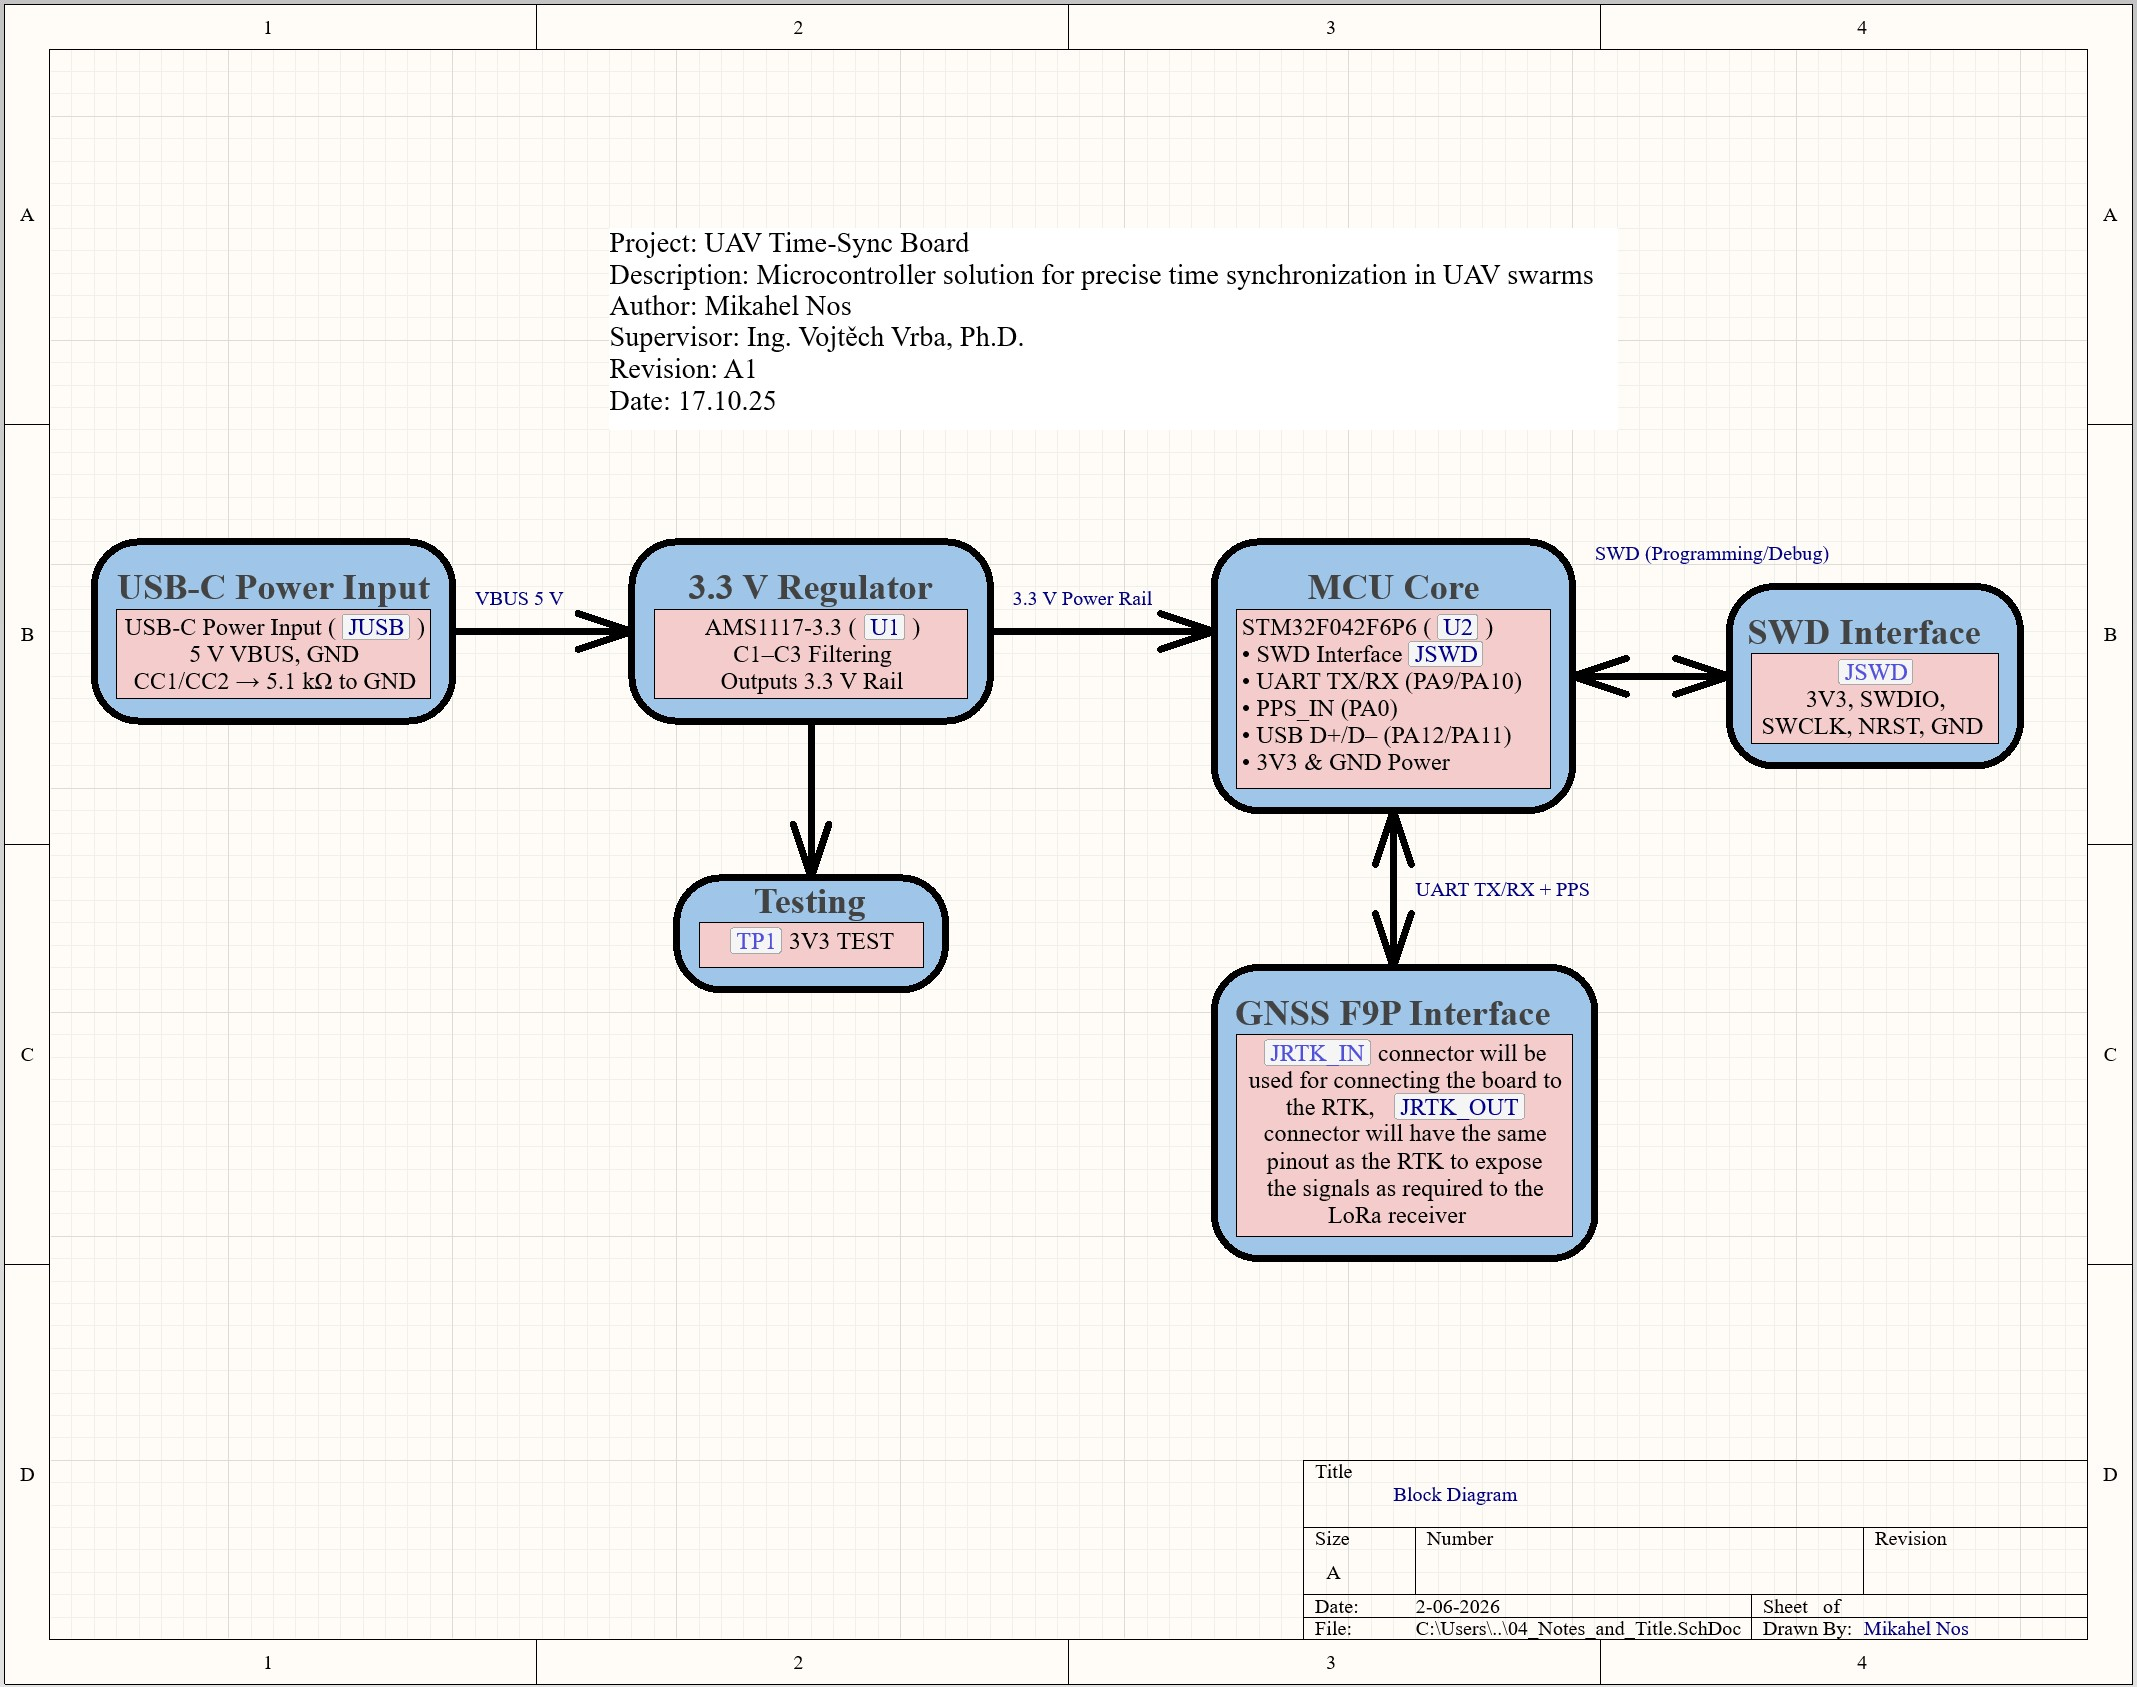
\includegraphics[width=1\textwidth]{fig/photos/block.jpg}
  \caption{System block diagram of the synchronization module, showing the DCF77 absolute-time input, RTK PPS timing input, STM32 firmware processing, UART diagnostic output, and ROS2 logging pipeline.}
  \label{fig:blockDiagram}
\end{figure}

\begin{sidewaysfigure}[p]
  \centering
  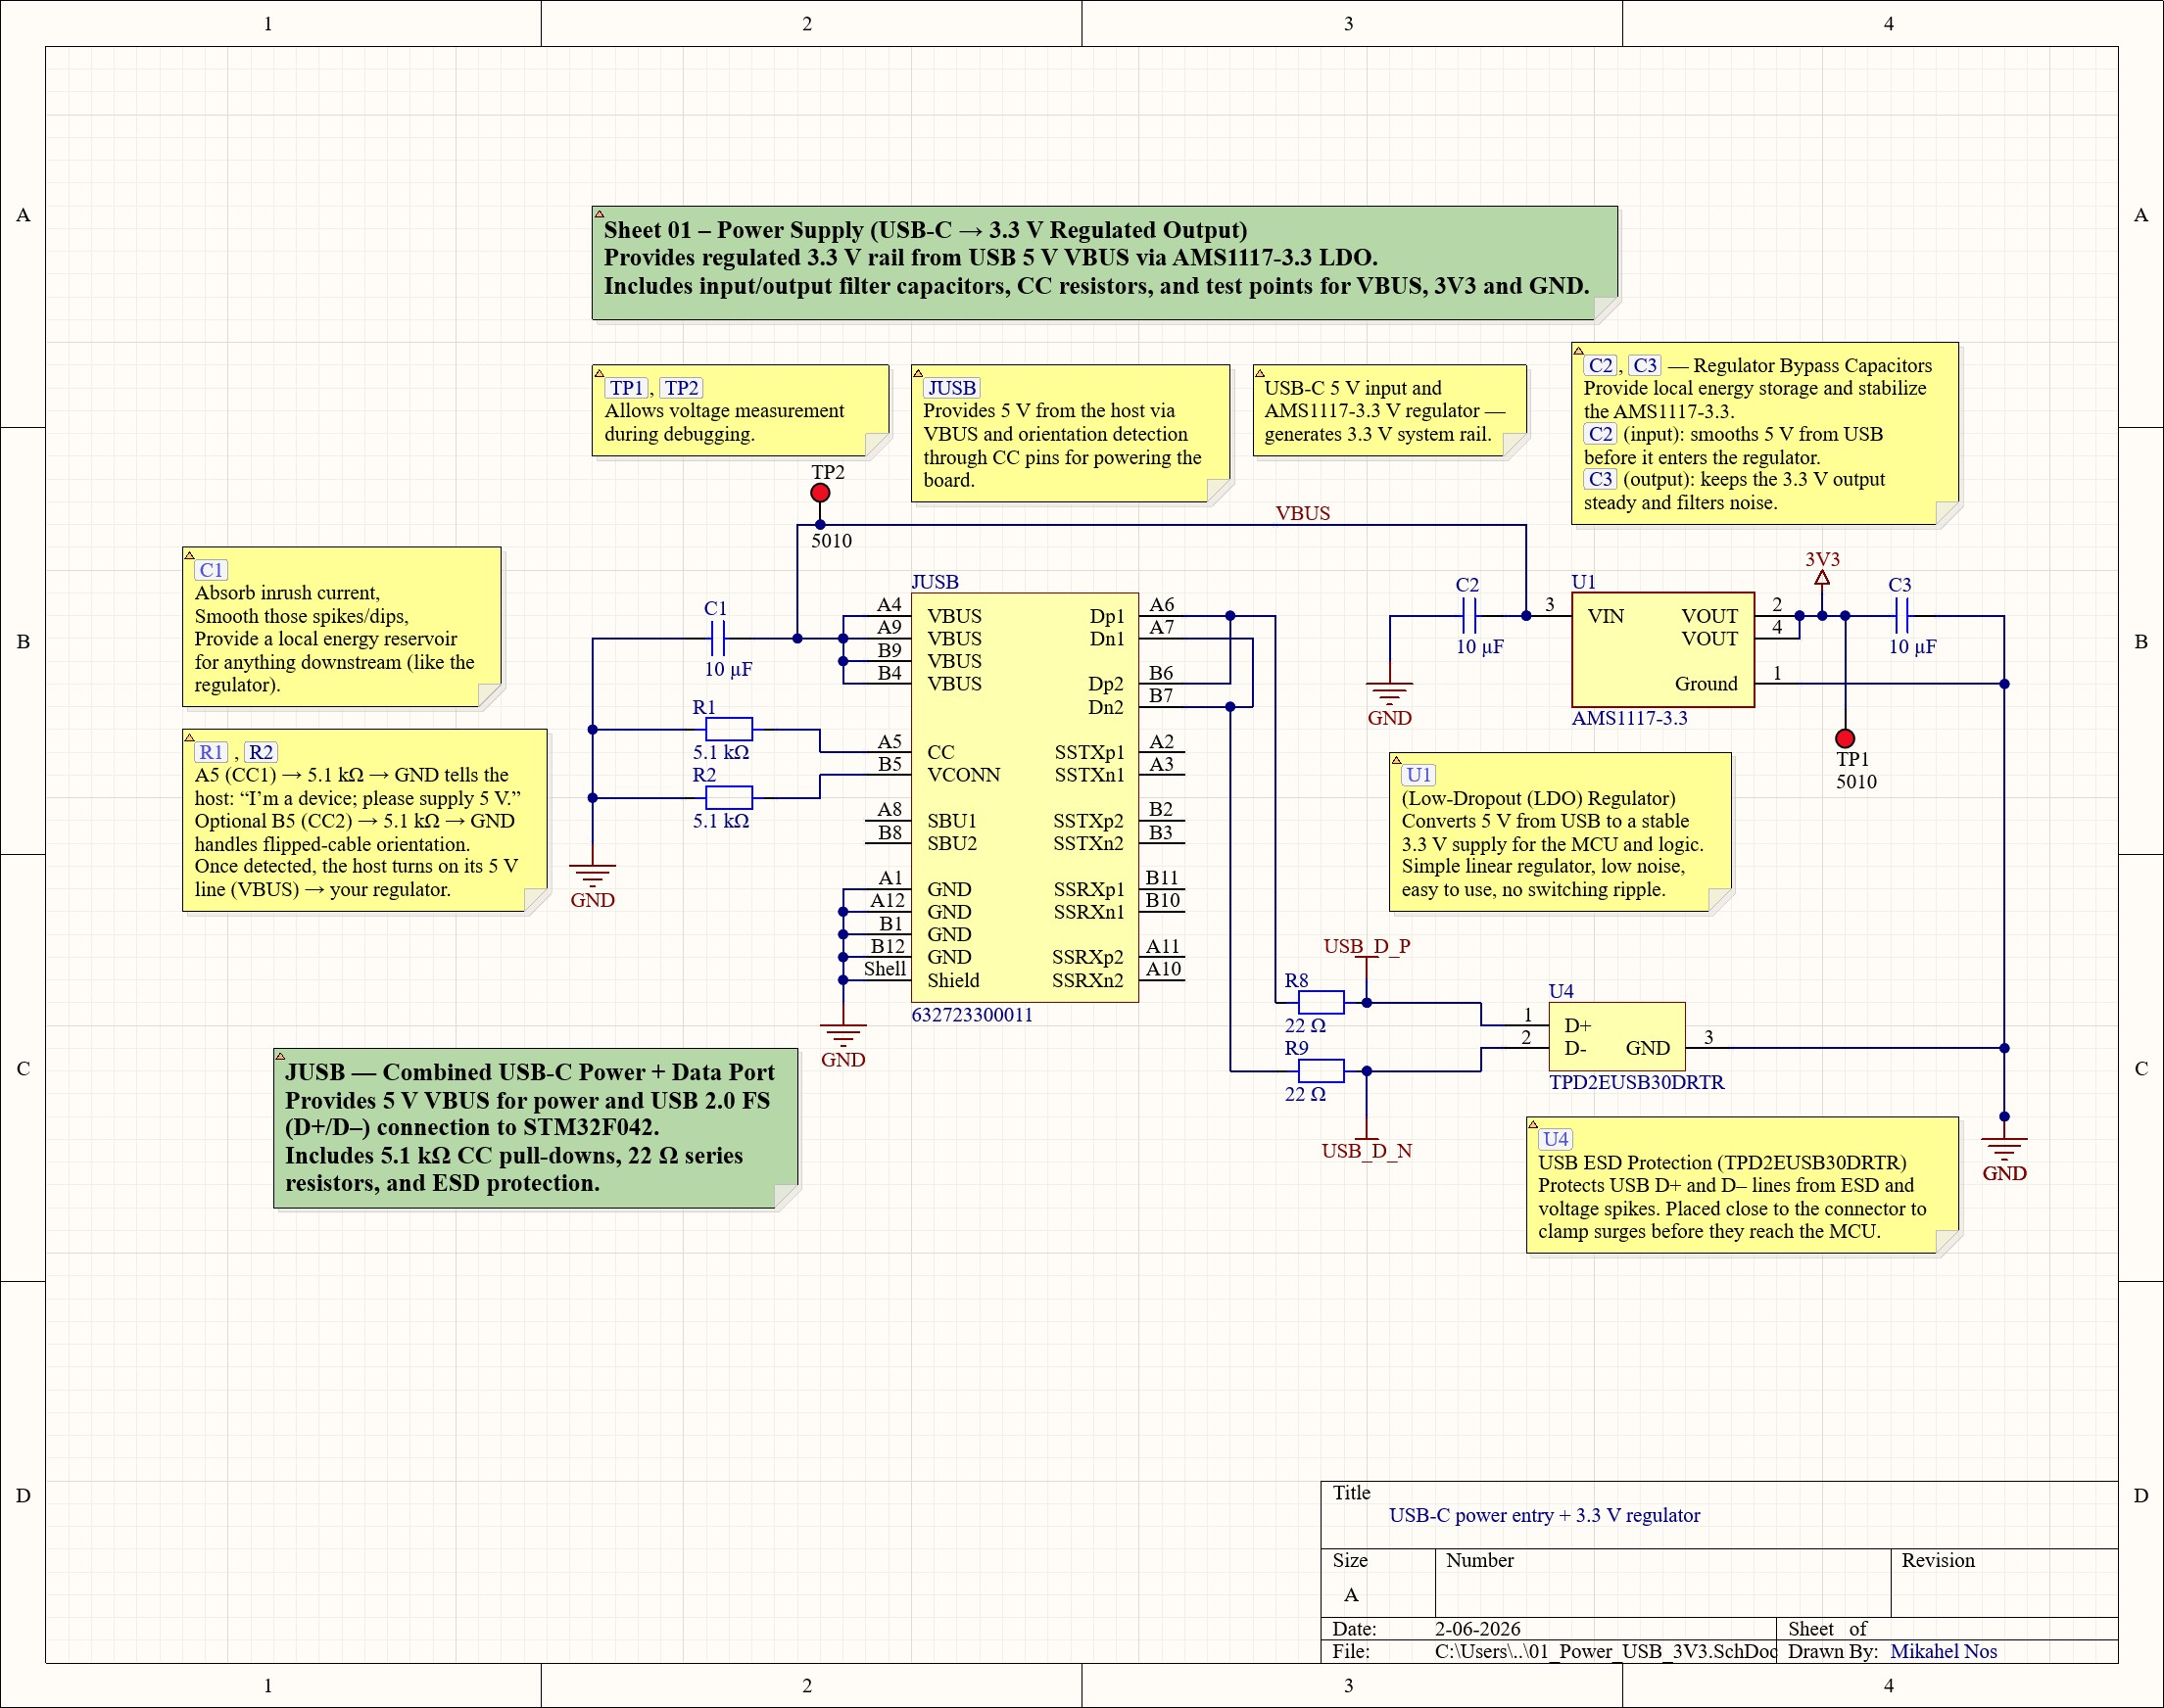
\includegraphics[width=0.9\textheight]{fig/photos/scm1.jpg}
  \caption{USB-C power entry and 3.3 V regulator schematic. This part of the design provides the regulated supply rail for the STM32 microcontroller and onboard digital circuitry.}
  \label{fig:usbPowerRegulator}
\end{sidewaysfigure}

\begin{sidewaysfigure}[p]
  \centering
  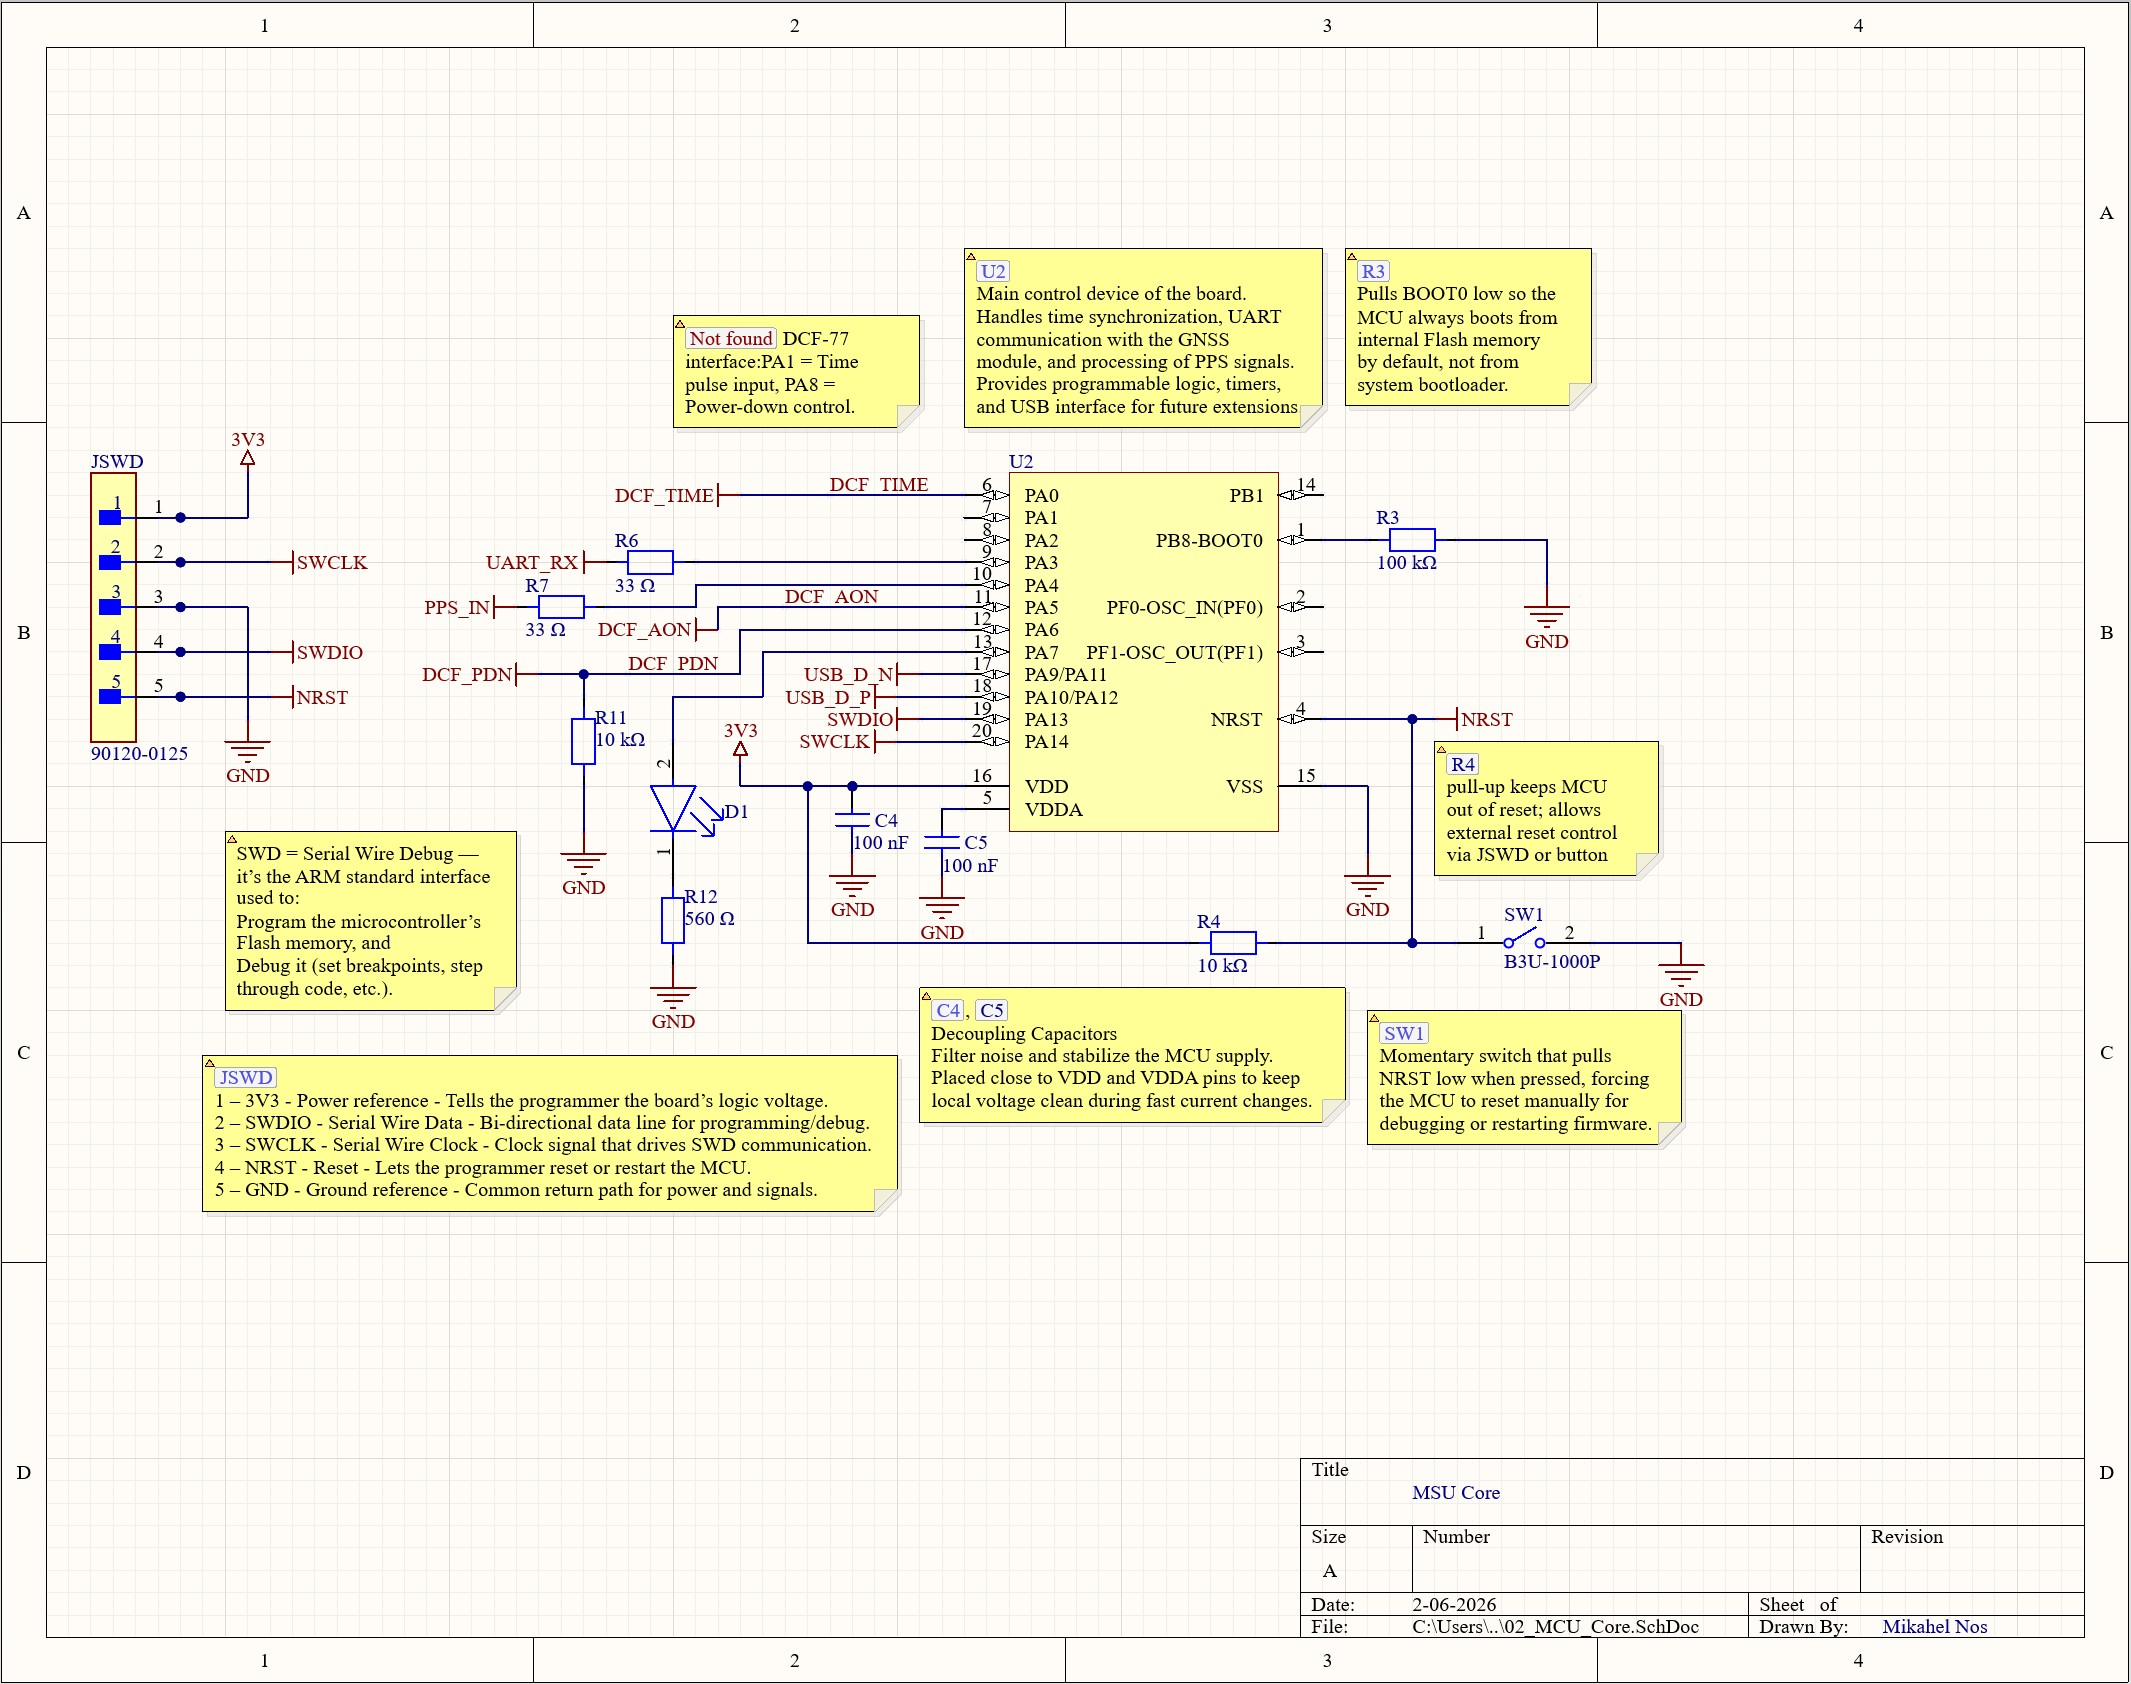
\includegraphics[width=0.9\textheight]{fig/photos/scm2.jpg}
  \caption{STM32F042F6P6 microcontroller core schematic with reset, boot, SWD debugging, UART communication, DCF77 input, and RTK PPS timing-signal connections.}
  \label{fig:mcuCore}
\end{sidewaysfigure}

\begin{sidewaysfigure}[p]
  \centering
  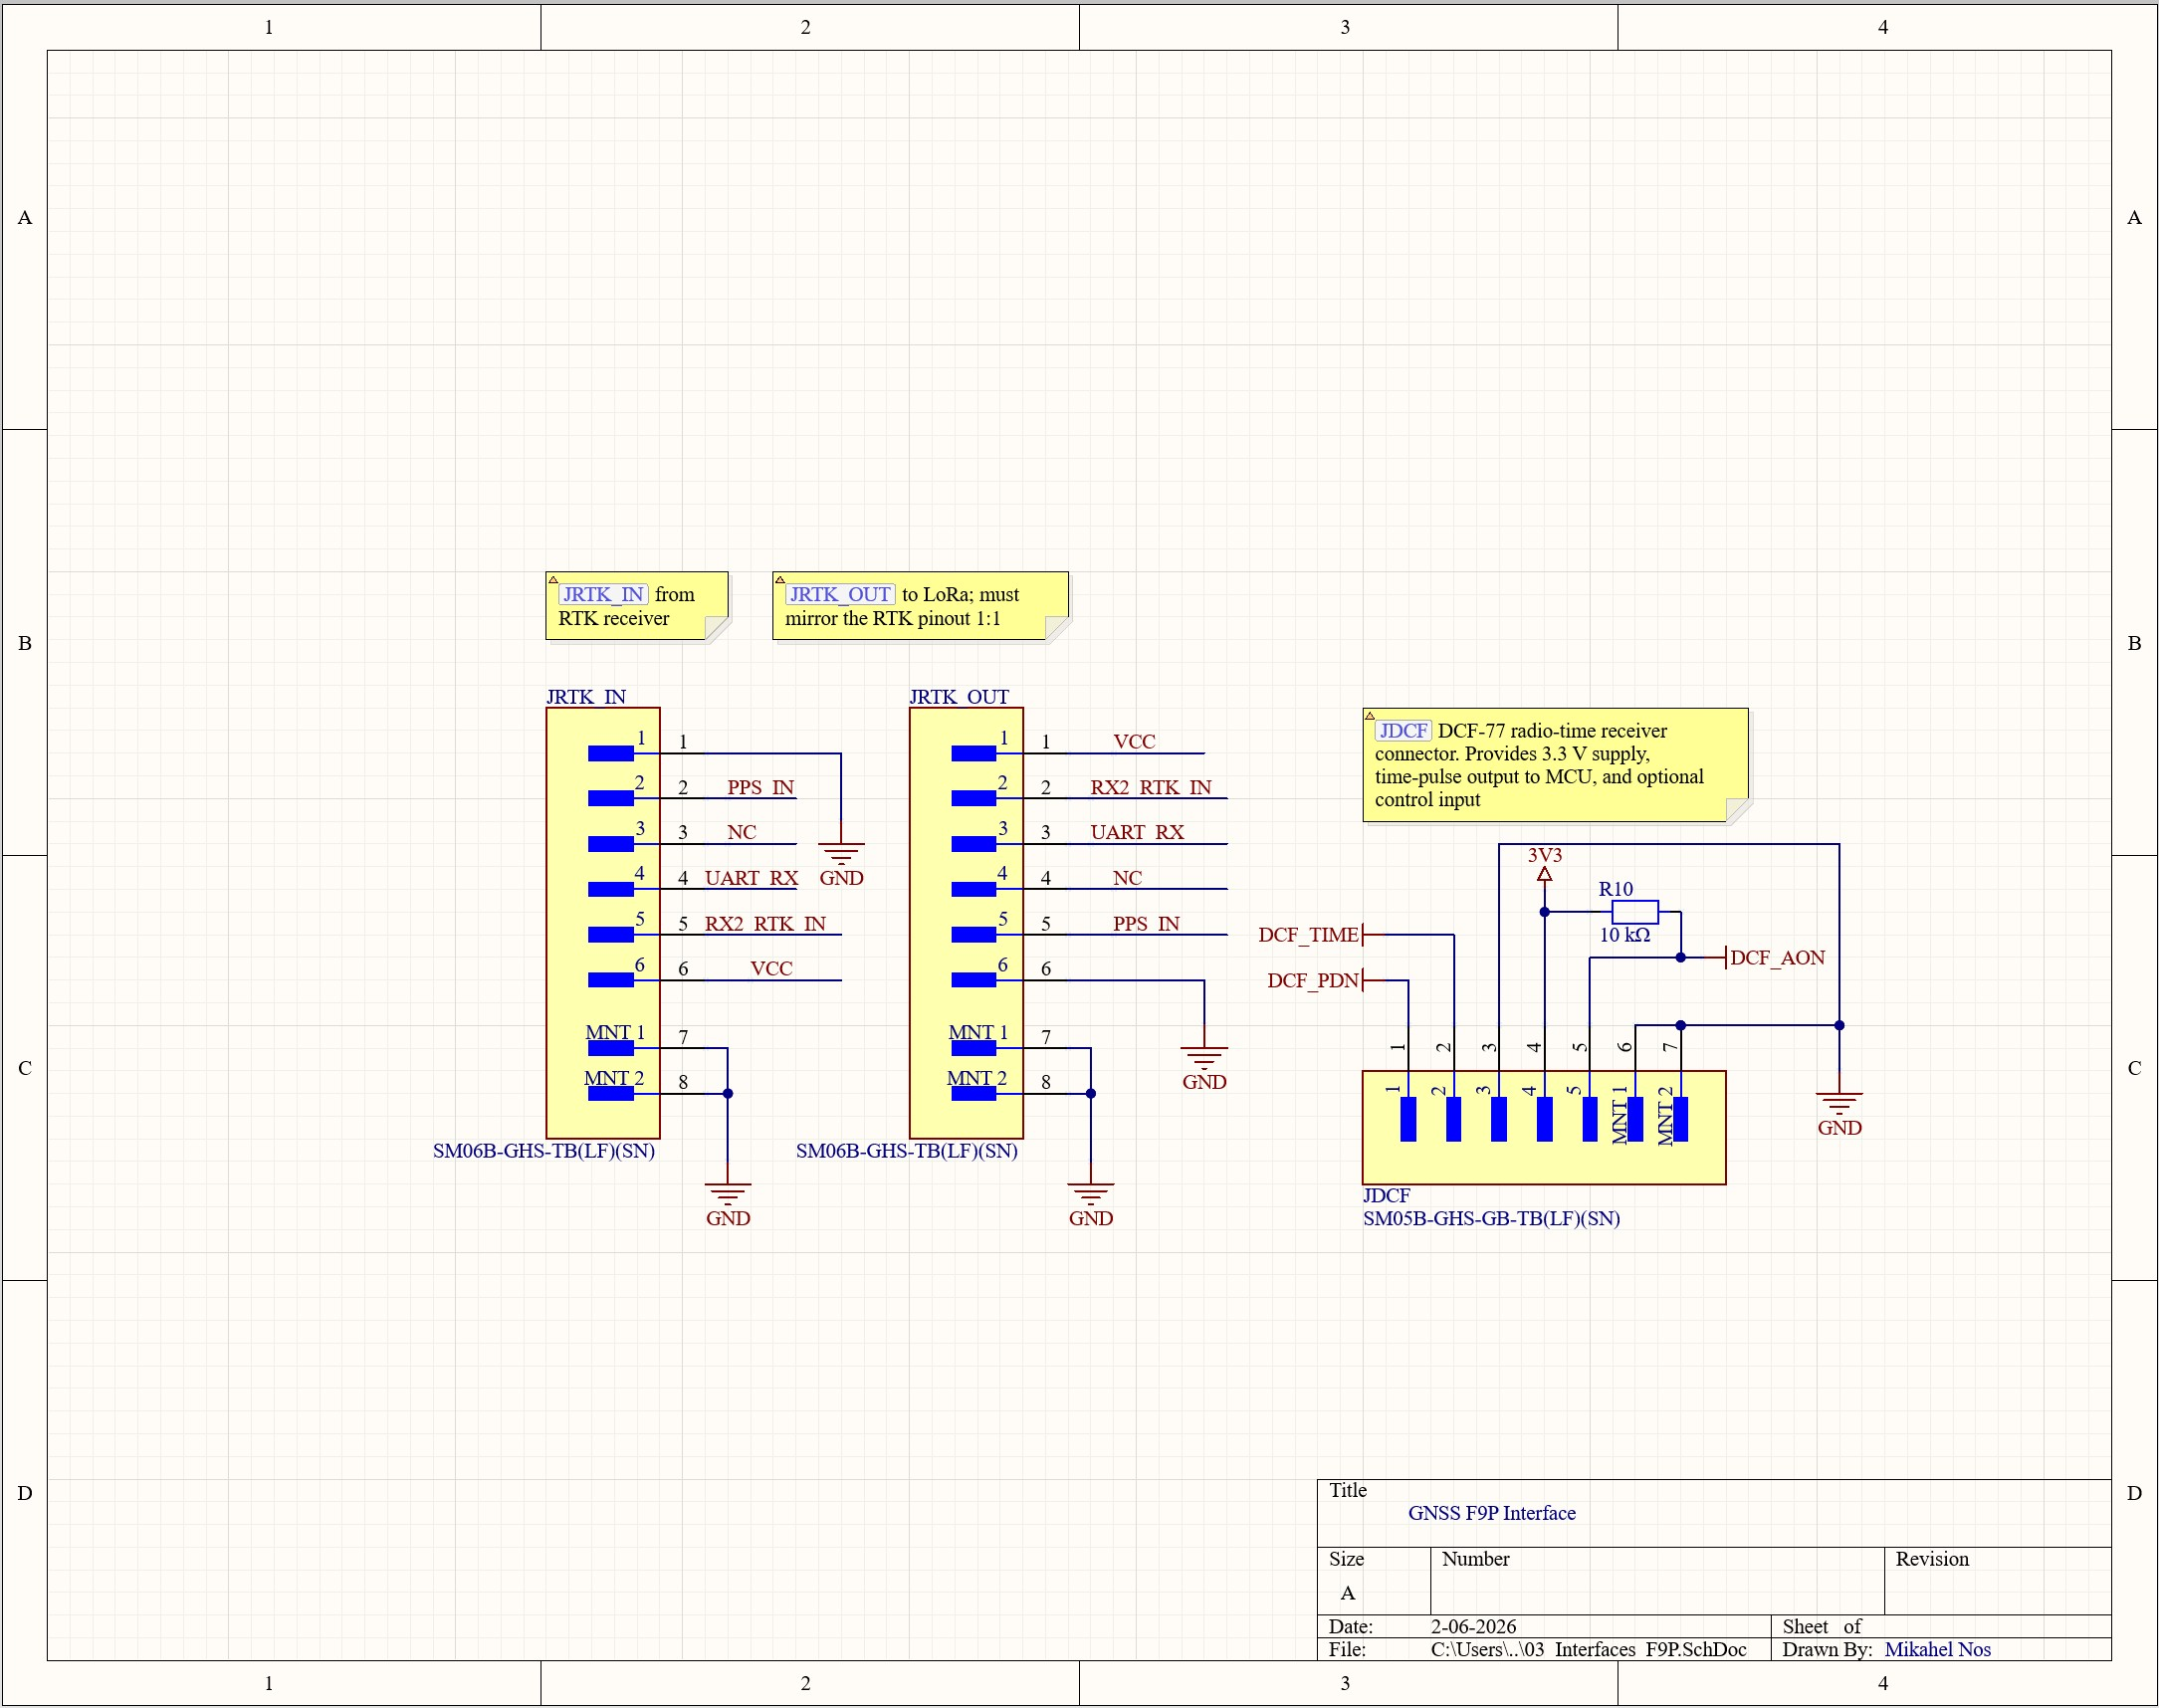
\includegraphics[width=0.9\textheight]{fig/photos/scm3.jpg}
  \caption{DCF77 and GNSS/RTK interface schematic, including timing-signal connectors, mirrored connector routing, and PPS signal path to the STM32 input.}
  \label{fig:timingInterfaces}
\end{sidewaysfigure}

\begin{figure}[htbp]
  \centering
  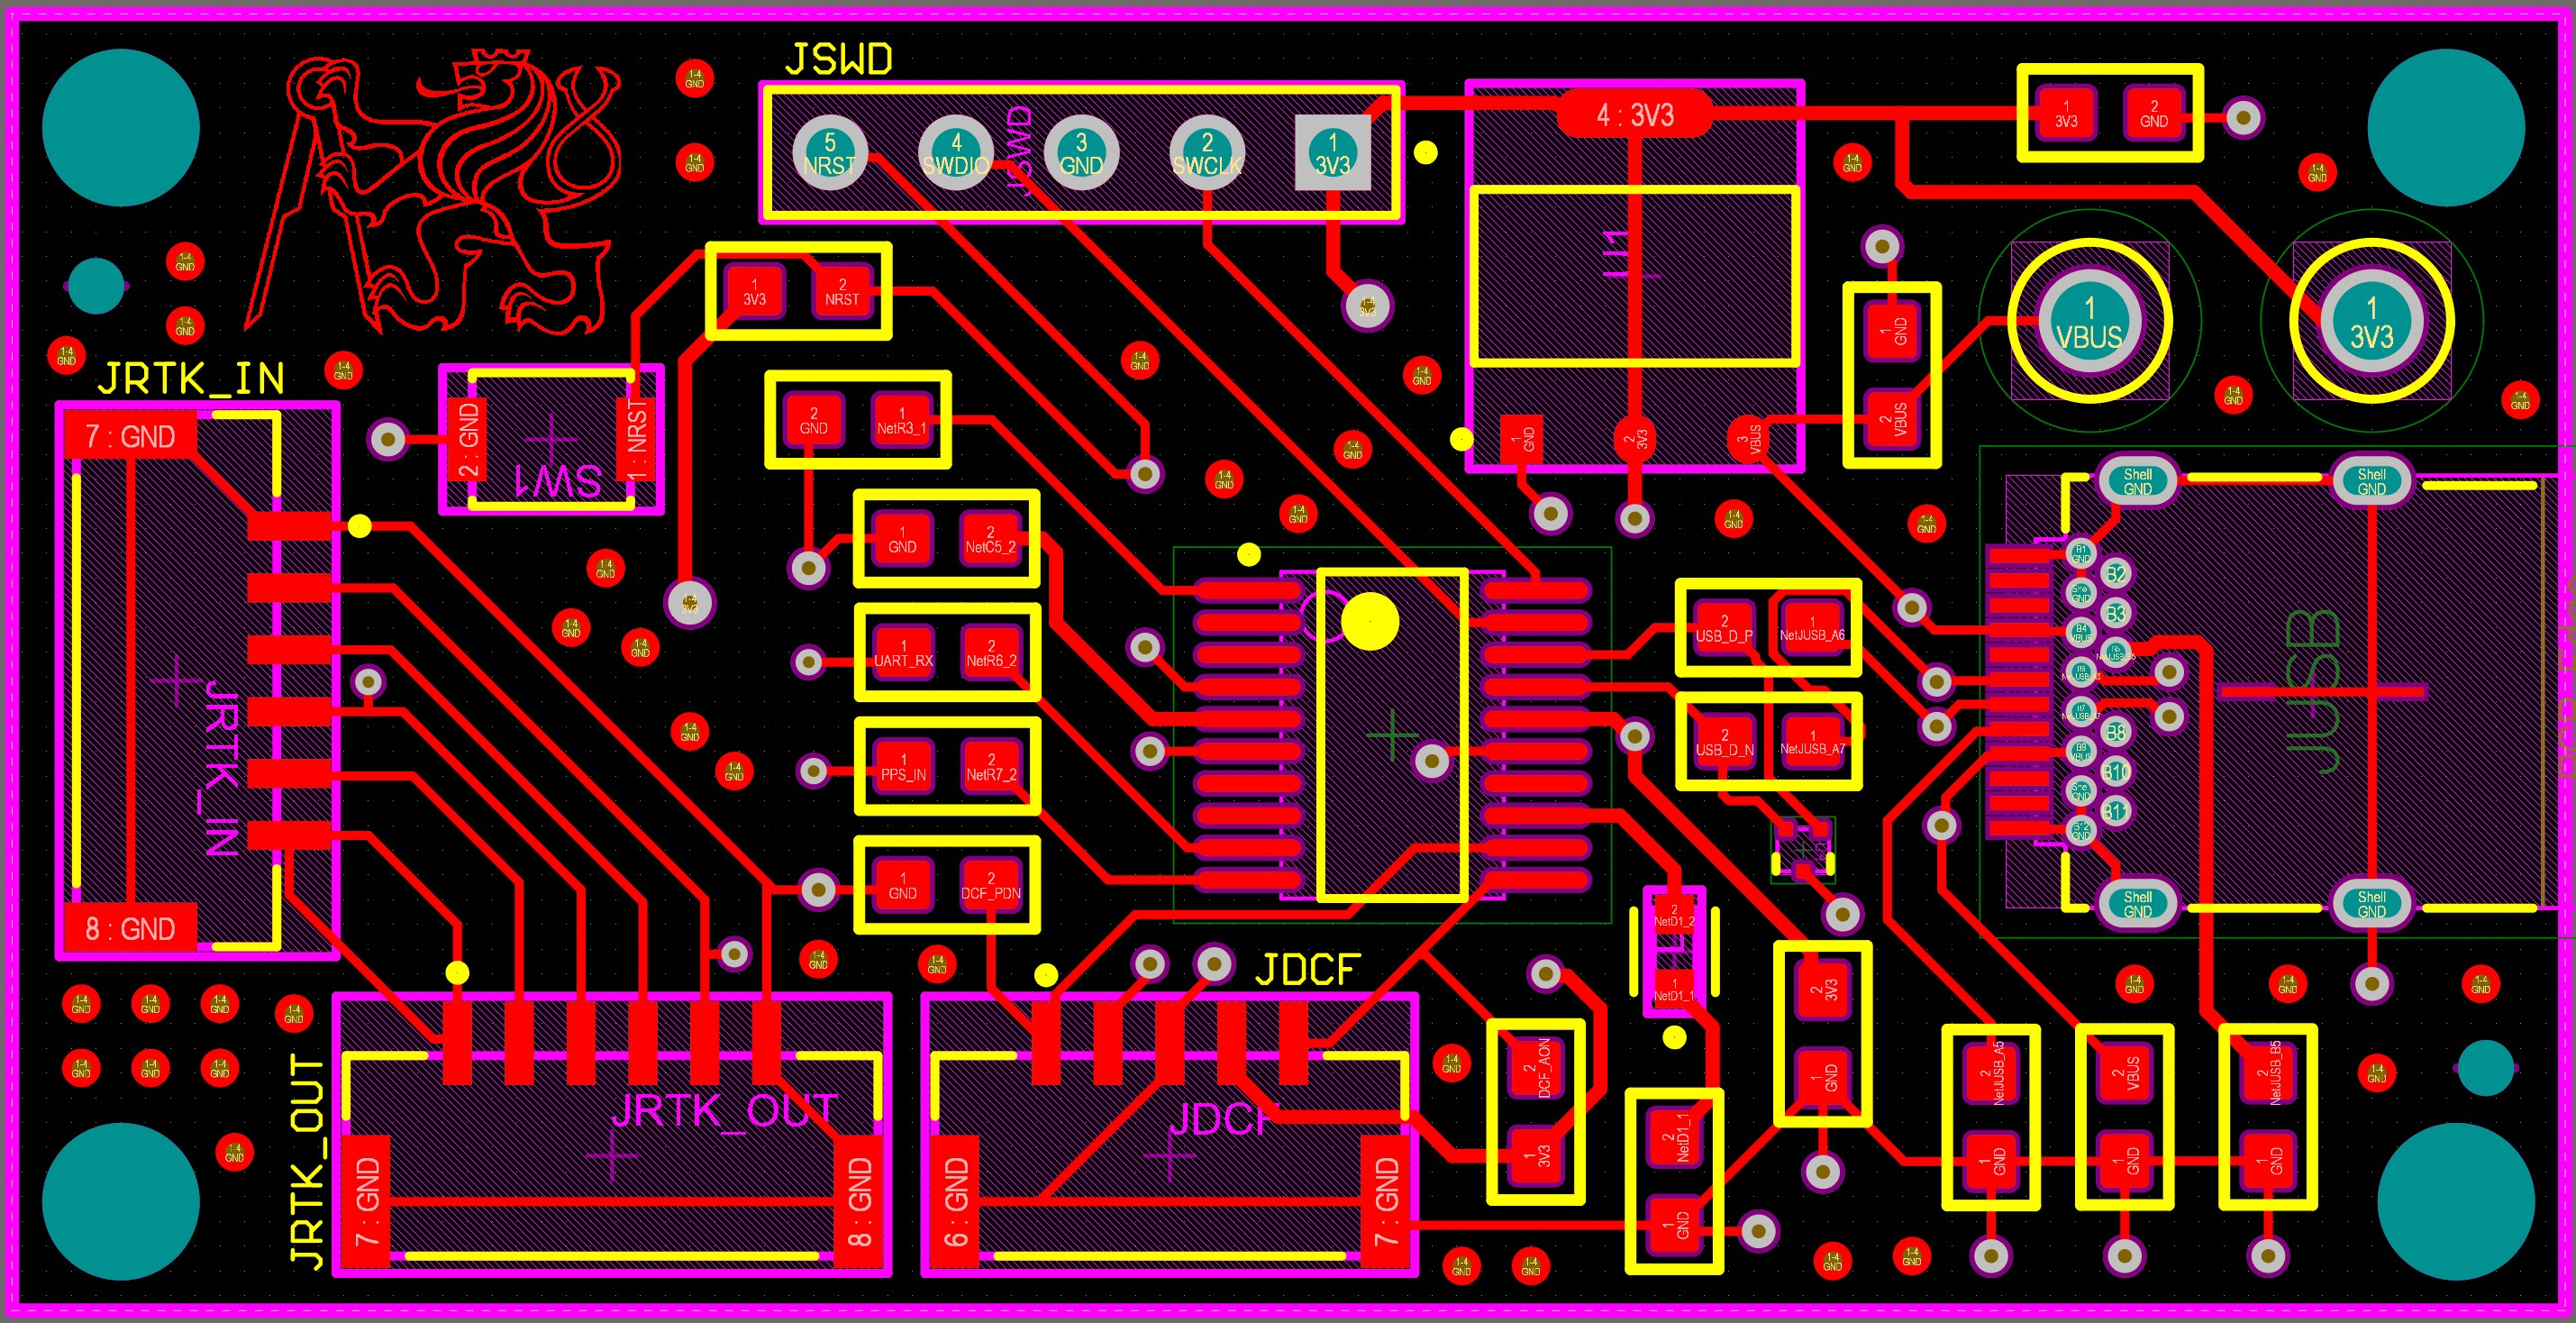
\includegraphics[width=1\textwidth]{fig/photos/pcb.jpg}
  \caption{PCB layout of the synchronization module, showing the compact four-layer board organization and routing of power, debugging, communication, and timing-signal sections.}
  \label{fig:pcbLayout}
\end{figure}

\begin{figure}[htbp]
  \centering
  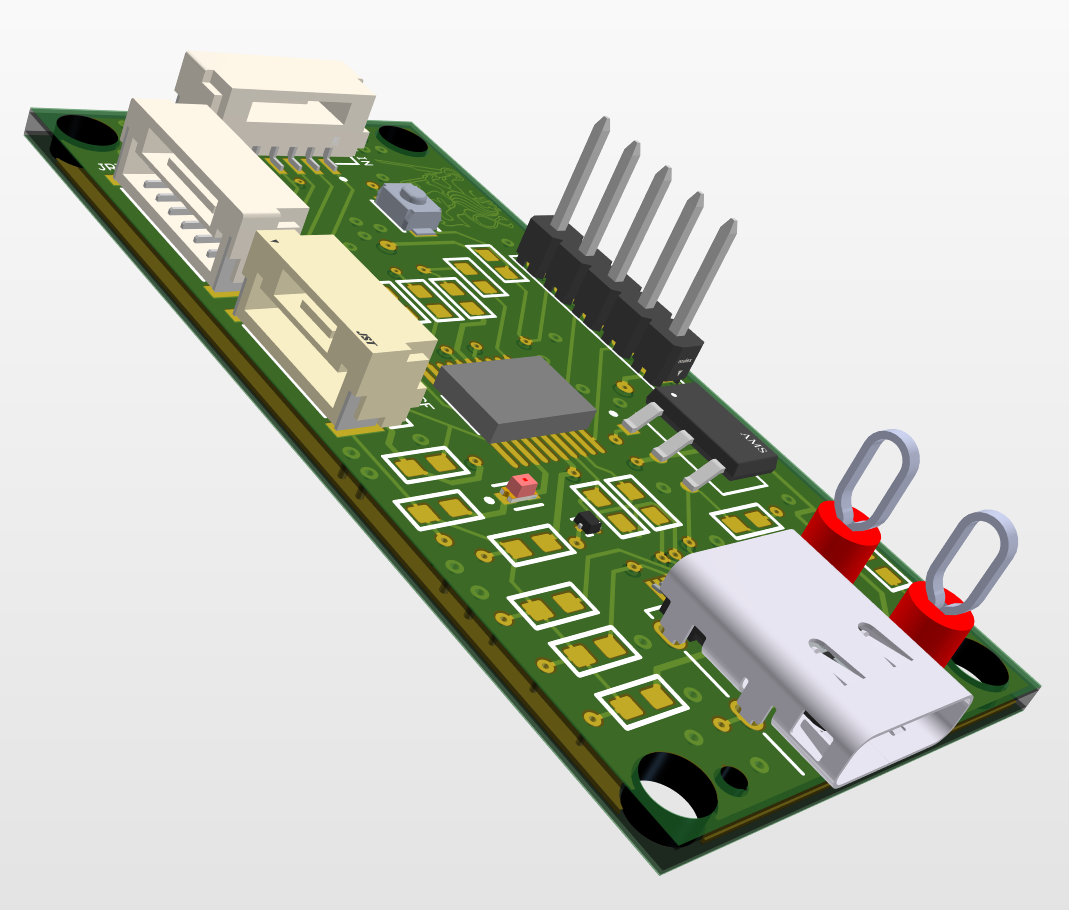
\includegraphics[width=0.9\textwidth]{fig/photos/pcb3d.png}
  \caption{3D render of the synchronization PCB, showing the physical component placement and expected assembled-board structure.}
  \label{fig:pcb3d}
\end{figure}

\chapter{Firmware Code Listings}
\label{app:firmwareCode}

This appendix contains selected firmware and ROS2 code listings used in the implemented synchronization system. The listings support the firmware description in Chapter~5 and document the main software blocks responsible for DCF77 decoding, software clock maintenance, RTK PPS processing, UART diagnostic output, and ROS2 logging.

\section{DCF77 Decoding and Validation}
\label{app:dcfDecoding}

\begin{lstlisting}[style=codeStyle, language=C, caption={DCF77 BCD decoding and frame validation functions.}, label={lst:dcfDecoding}]
// Decode DCF77 BCD section into integer value
uint8_t decode_dcf_section(volatile uint8_t *bits, int start, int end) {
    uint8_t result = 0;
    // Standard BCD weights for DCF77
    uint8_t weights[] = {1, 2, 4, 8, 10, 20, 40};

    for (int i = 0; i <= (end - start); i++) {
        if (bits[start + i]) {
            result += weights[i];
        }
    }
    return result;
}

uint8_t decode_dcf_year(uint8_t *bits)
{
    uint8_t w[] = {1, 2, 4, 8, 10, 20, 40, 80};
    uint8_t res = 0;

    for (int i = 0; i < 8; i++)
        if (bits[50 + i]) res += w[i];

    return res;
}

// Validate full DCF77 parity frame
uint8_t dcf_check_parity_all(uint8_t *bits)
{
    uint8_t p;

    p = 0;
    for (int i = 21; i <= 27; i++)
        p \^= bits[i];
    if (p != bits[28]) return 0;

    p = 0;
    for (int i = 29; i <= 34; i++)
        p \^= bits[i];
    if (p != bits[35]) return 0;

    p = 0;
    for (int i = 36; i <= 57; i++)
        p \^= bits[i];
    if (p != bits[58]) return 0;

    return 1;
}

uint8_t dcf_data_is_valid(uint8_t *bits)
{
    uint8_t m  = decode_dcf_section(bits, 21, 27);
    uint8_t h  = decode_dcf_section(bits, 29, 34);
    uint8_t d  = decode_dcf_section(bits, 36, 41);
    uint8_t mo = decode_dcf_section(bits, 45, 49);
    uint8_t y  = decode_dcf_year(bits);

    if (m > 59) return 0;
    if (h > 23) return 0;
    if (mo < 1 || mo > 12) return 0;
    if (d < 1 || d > days_in_month(mo, 2000 + y)) return 0;

    // After first valid sync, reject impossible date jumps
    if (clock_valid)
    {
        if (y != clk_year) return 0;
        if (mo != clk_month) return 0;
        if (d != clk_day) return 0;
    }

    return 1;
}

\end{lstlisting}

\section{Software Real-Time Clock}
\label{app:softwareRtc}

\begin{lstlisting}[style=codeStyle, language=C, caption={Software RTC functions for calendar handling and one-second increments.}, label={lst:softwareRtc}]
uint8_t is_leap_year(uint16_t year)
{
    if ((year % 400) == 0) return 1;
    if ((year % 100) == 0) return 0;
    if ((year % 4) == 0) return 1;
    return 0;
}

uint8_t days_in_month(uint8_t month, uint16_t year)
{
    switch (month)
    {
        case 1:  return 31;
        case 2:  return is_leap_year(year) ? 29 : 28;
        case 3:  return 31;
        case 4:  return 30;
        case 5:  return 31;
        case 6:  return 30;
        case 7:  return 31;
        case 8:  return 31;
        case 9:  return 30;
        case 10: return 31;
        case 11: return 30;
        case 12: return 31;
        default: return 31;
    }
}

// Increment internal software clock by one second
void clock_add_one_second(void)
{
    clk_sec++;

    if (clk_sec < 60) return;
    clk_sec = 0;
    clk_min++;

    if (clk_min < 60) return;
    clk_min = 0;
    clk_hour++;

    if (clk_hour < 24) return;
    clk_hour = 0;
    clk_day++;

    uint16_t full_year = 2000 + clk_year;
    if (clk_day <= days_in_month(clk_month, full_year)) return;
    clk_day = 1;
    clk_month++;

    if (clk_month <= 12) return;
    clk_month = 1;
    clk_year++;
}

void apply_pending_dcf_sync(void)
{
	clk_min = pending_min;
	clk_hour = pending_hour;
	clk_day = pending_day;
	clk_month = pending_month;
	clk_year = pending_year;
	clk_sec = 0;

    clock_valid = 1;
    pending_sync = 0;
    use_rtk_pps_clock = 1;

    last_clock_tick_ms = __HAL_TIM_GET_COUNTER(&htim2);
    dcf_second_tick_ms = HAL_GetTick();

    last_dcf_hour  = clk_hour;
    last_dcf_min   = clk_min;
    last_dcf_day   = clk_day;
    last_dcf_month = clk_month;
    last_dcf_year  = clk_year;

    update_debug_time_string();

    dcf_sync_done = 1;
    last_valid_dcf_ms = HAL_GetTick();
}

\end{lstlisting}

\section{DCF77 Clock Synchronization}
\label{app:dcfClockSync}

\begin{lstlisting}[style=codeStyle, language=C, caption={DCF77 synchronization and safe clock-correction functions.}, label={lst:dcfClockSync}]
void sync_clock_from_dcf(uint8_t *bits)
{
    pending_min   = decode_dcf_section(bits, 21, 27);
    pending_hour  = decode_dcf_section(bits, 29, 34);
    pending_day   = decode_dcf_section(bits, 36, 41);
    pending_month = decode_dcf_section(bits, 45, 49);
    pending_year  = decode_dcf_year(bits);

    pending_sync = 1;
}

void correct_clock_from_dcf_soft(uint8_t *bits)
{
    uint8_t dcf_min  = decode_dcf_section(bits, 21, 27);
    uint8_t dcf_hour = decode_dcf_section(bits, 29, 34);
    uint8_t dcf_day  = decode_dcf_section(bits, 36, 41);
    uint8_t dcf_mon  = decode_dcf_section(bits, 45, 49);
    uint8_t dcf_year = decode_dcf_year(bits);

    // Save last valid DCF sync info
    last_dcf_min   = dcf_min;
    last_dcf_hour  = dcf_hour;
    last_dcf_day   = dcf_day;
    last_dcf_month = dcf_mon;
    last_dcf_year  = dcf_year;

    dcf_sync_done = 1;

    // Only correct if date/hour/minute match current clock.
    // This prevents bad jumps.
    if (dcf_year != clk_year) return;
    if (dcf_mon  != clk_month) return;
    if (dcf_day  != clk_day) return;
    if (dcf_hour != clk_hour) return;
    if (dcf_min  != clk_min) return;

    // At valid DCF minute boundary, seconds should be near 0.
    // If internal clock is slightly ahead, pull it back by 1 second.
    if (last_dcf_year == clk_year &&
        last_dcf_month == clk_month &&
        last_dcf_day == clk_day &&
        last_dcf_hour == clk_hour &&
        last_dcf_min == clk_min)
    {
        if (clk_sec >= 1 && clk_sec <= 10)
        {
            clk_sec = 0;
            last_clock_tick_ms = __HAL_TIM_GET_COUNTER(&htim2);
        }
        else if (clk_sec >= 50)
        {
            clk_sec = 0;
            last_clock_tick_ms = __HAL_TIM_GET_COUNTER(&htim2);
        }
    }

    // If somehow seconds are 59, push to 0.
    if (clk_sec == 59)
    {
        clk_sec = 0;
    }

    update_debug_time_string();
    last_valid_dcf_ms = HAL_GetTick();
}

void check_dcf_sync_timeout(void)
{
    if (clock_valid)
    {
        if ((HAL_GetTick() - last_valid_dcf_ms) > 300000) // 5 minutes
        {
            update_debug_time_string();
        }
    }
}
\end{lstlisting}

\section{UART Diagnostic Message Generation}
\label{app:uartDiagnostics}

\begin{lstlisting}[style=codeStyle, language=C, caption={UART diagnostic string generation with synchronization state and RTK PPS values.}, label={lst:uartDiagnostics}]
void update_debug_time_string(void)
{
	if (clock_valid)
	{
		snprintf(debug_time_str, sizeof(debug_time_str),
		         "%02u:%02u:%02u - %02u.%02u.20%02u - %s - SYNC=%d - LASTDCF=%02u.%02u.20%02u_%02u:%02u - RTK_PPS=%lu - RTK_DELTA=%lums - RTK_DIFF=%ldms\r\n",
		         clk_hour, clk_min, clk_sec,
		         clk_day, clk_month, clk_year,
		         PCB_ID, clock_valid,
		         last_dcf_day, last_dcf_month, last_dcf_year,
		         last_dcf_hour, last_dcf_min,
		         rtk_pps_count,
		         rtk_pps_delta_ms,
		         rtk_dcf_diff_ms);
	}
	else
	{
	    snprintf(debug_time_str, sizeof(debug_time_str),
	             "NO_SYNC - %s - RTK_PPS=%lu - RTK_DELTA=%lums - RTK_DIFF=%ldms\r\n",
	             PCB_ID,
	             rtk_pps_count,
	             rtk_pps_delta_ms,
	             rtk_dcf_diff_ms);
	}
}
\end{lstlisting}

\section{Main Firmware Loop}
\label{app:mainLoop}

\begin{lstlisting}[style=codeStyle, language=C, caption={Main firmware loop handling fallback timing and deferred UART transmission.}, label={lst:mainLoop}]
  /* USER CODE BEGIN WHILE */
  while (1)
  {
	check_dcf_sync_timeout();

	volatile uint32_t now_ms = __HAL_TIM_GET_COUNTER(&htim2);

	if ((now_ms - last_clock_tick_ms) >= 1000)
	{
	    last_clock_tick_ms += 1000;

	    if (!use_rtk_pps_clock)
	    {
	        clock_add_one_second();
	        HAL_GPIO_TogglePin(TEST_GPIO_Port, TEST_Pin);
	        update_debug_time_string();
	        pps_print_pending = 1;
	    }
	}

	if (pps_print_pending)
	{
	    pps_print_pending = 0;

	    HAL_UART_Transmit(&huart2,
	                      (uint8_t*)debug_time_str,
	                      strlen(debug_time_str),
	                      HAL_MAX_DELAY);
	}

    /* USER CODE END WHILE */

    /* USER CODE BEGIN 3 */
  }
  /* USER CODE END 3 */
\end{lstlisting}

\section{External Interrupt Callback}
\label{app:extiCallback}

\begin{lstlisting}[style=codeStyle, language=C, caption={External interrupt callback for DCF77 edge processing and RTK PPS handling.}, label={lst:extiCallback}]
/* USER CODE BEGIN 4 */

/* ============================================================================
 * INTERRUPTS AND CALLBACKS
 * ==========================================================================*/

void HAL_GPIO_EXTI_Callback(uint16_t GPIO_Pin)
{
	// DCF77 edge processing
    if (GPIO_Pin == GPIO_PIN_0)
    {
    	uint32_t now_ms = __HAL_TIM_GET_COUNTER(&htim2);

        static uint32_t last_any_edge = 0;
        if (now_ms - last_any_edge < 15) return; 
        last_any_edge = now_ms;

        GPIO_PinState pin_state = HAL_GPIO_ReadPin(GPIOA, GPIO_PIN_0);

        if (pin_state == GPIO_PIN_SET)
        {
            // rising edge

            if (last_rise_time != 0)
            {
                last_rise_delta = now_ms - last_rise_time;


                if (last_rise_delta > 1500)
                {
                	if (pending_sync)
                	{
                	    apply_pending_dcf_sync();
                	}
                	    minute_detected = 1;
                	    second = 0;
                	    parity = 0;

                	    for (int i = 0; i < 59; i++)
                	        bits[i] = 0;
                }
            }

            rise_time = now_ms;
            last_rise_time = now_ms;
        }
        else
        {
            // falling edge
            last_width = now_ms - rise_time;

        	if (!minute_detected) return;

        	uint8_t bit = 2;
            if (last_width >= 90 && last_width <= 155) bit = 0;
            else if (last_width >= 180 && last_width <= 260) bit = 1;
            else
            {
                dcf_bad_width_count++;
                return;
            }

        	if (second < 59)
        	{
				bits[second++] = bit;

				if (second == 59)
				{
				    parity = dcf_check_parity_all(bits);
				    minute_detected = 0;

				    if (!parity)
				    {
				        dcf_parity_fail_count++;
				    }
				    else if (!dcf_data_is_valid(bits))
				    {
				        dcf_data_fail_count++;
				    }
				    else
				    {
				        dcf_ok_count++;

				        if (!clock_valid)
				            sync_clock_from_dcf(bits);
				        else
				            correct_clock_from_dcf_soft(bits);
				    }
				}
        	}
        }
    }
    // RTK PPS processing
    if (GPIO_Pin == GPIO_PIN_4)
    {
        uint32_t now = HAL_GetTick();
        uint32_t delta = now - rtk_pps_last_ms;

        if (delta > 990 && delta < 1010)
        {
            rtk_pps_delta_ms = delta;
            rtk_pps_last_ms = now;
            rtk_pps_tick_ms = now;
            rtk_pps_count++;

            if (use_rtk_pps_clock && clock_valid)
            {
                clock_add_one_second();
                dcf_second_tick_ms = now;
                update_debug_time_string();
                pps_print_pending = 1;
            }

            rtk_dcf_diff_ms = (int32_t)rtk_pps_tick_ms - (int32_t)dcf_second_tick_ms;

            while (rtk_dcf_diff_ms > 500) rtk_dcf_diff_ms -= 1000;
            while (rtk_dcf_diff_ms < -500) rtk_dcf_diff_ms += 1000;
        }
        else if (delta > 1200)
        {
            rtk_pps_last_ms = now;
        }
    }
}

/* USER CODE END 4 */
\end{lstlisting}

\section{ROS2 Serial Node}
\label{app:rosSerialNode}

\begin{lstlisting}[style=codeStyle, language=Python, caption={ROS2 serial node for reading UART synchronization messages and publishing them to ROS2 topics.}, label={lst:rosSerialNode}]
import rclpy
import csv
import os
from rclpy.node import Node
import serial

from std_msgs.msg import String


class SerialNode(Node):
    def __init__(self):
        super().__init__('serial_node')
        self.get_logger().info('Serial node started')
        self.declare_parameter('port', '/dev/ttyUSB0')
        self.declare_parameter('topic', '/serial_raw')

        self.port = self.get_parameter('port').value
        self.topic = self.get_parameter('topic').value
        self.csv_path = os.path.expanduser('~/ros2_ws/dcf_log.csv')
        self.csv_file = open(self.csv_path, 'a', newline='')
        self.csv_writer = csv.writer(self.csv_file)

        if self.csv_file.tell() == 0:
            self.csv_writer.writerow(['ros_time_sec', 'ros_time_nsec', 'raw_line'])

        self.get_logger().info(f'Logging to {self.csv_path}')

        self.raw_publisher = self.create_publisher(String, self.topic, 10)

        self.ser = None

        try:
            self.ser = serial.Serial(self.port, 9600, timeout=0.1)
            self.get_logger().info('Serial port opened')
        except Exception as e:
            self.get_logger().error(f"Failed to open serial port {self.port}: {e}")
            self.ser = None

        self.timer = self.create_timer(0.05, self.timer_callback)

    def parse_dcf_time_line(self, line):
        parts = line.split()

        if len(parts) >= 9 and parts[1] == '-' and parts[3] == '-' and parts[5] == '-' and parts[7] == '-':
            time_str = parts[0]
            date_str = parts[2]
            pcb_id = parts[4]
            sync = parts[6]
            lastdcf = parts[8]

            return f'{time_str} {date_str} {pcb_id} {sync} {lastdcf}'

        return None

    def timer_callback(self):
        if not self.ser:
            self.get_logger().info('No serial port')
            return

        try:
            line = self.ser.readline().decode('utf-8', errors='ignore').strip()

            if not line:
                return

            self.get_logger().info(f'Received: {line}')
            
            now = self.get_clock().now().to_msg()

            self.csv_writer.writerow([
                now.sec,
                now.nanosec,
                line
            ])
            self.csv_file.flush()

            raw_msg = String()
            raw_msg.data = line
            self.raw_publisher.publish(raw_msg)
            self.get_logger().info(f'Published raw: {line}')

            parsed = self.parse_dcf_time_line(line)

            if parsed is not None:
                self.get_logger().info(f'Parsed DCF time: {parsed}')

        except Exception as e:
            self.get_logger().warn(f'Read error: {e}')


def main(args=None):
    rclpy.init(args=args)
    node = SerialNode()
    rclpy.spin(node)
    node.destroy_node()
    rclpy.shutdown()


if __name__ == '__main__':
    main()
\end{lstlisting}

\section{ROS2 Comparison Node}
\label{app:rosCompareNode}

\begin{lstlisting}[style=codeStyle, language=Python, caption={ROS2 comparison node for evaluating two synchronization streams.}, label={lst:rosCompareNode}]
class DcfCompareNode(Node):
    def __init__(self):
        super().__init__('dcf_compare')
        self.create_subscription(String, '/dcf_a', self.cb_a, 10)
        self.create_subscription(String, '/dcf_b', self.cb_b, 10)
        self.csv_path = os.path.expanduser('~/ros2_ws/dcf_compare_log.csv')
        self.csv_file = open(self.csv_path, 'a', newline='')
        self.csv_writer = csv.writer(self.csv_file)
        self.status_timer = self.create_timer(1.0, self.status_check)
        self.selected_pub = self.create_publisher(String, "/dcf_time_selected", 10)
        self.last_a_raw = None
        self.last_b_raw = None
        self.last_published_selected_time = None

        if self.csv_file.tell() == 0:
            self.csv_writer.writerow([
                'ros_time',
                'dcf_diff_s',
                'arrival_diff_ms',
                'rtk_diff_a_ms',
                'rtk_diff_b_ms',
                'rtk_delta_a_ms',
                'rtk_delta_b_ms'
            ])

        self.get_logger().info(f'Logging comparison to {self.csv_path}')

        self.last_a_time = None
        self.last_b_time = None
        self.last_a_ros = None
        self.last_b_ros = None
        self.last_a_age = None
        self.last_b_age = None
        
    def destroy_node(self):
        if self.csv_file:
            self.csv_file.close()
        super().destroy_node()       
        
    def status_check(self):
        now = self.get_clock().now().nanoseconds / 1e9

        if self.last_a_ros is None:
            status_a = "NO DATA"
        elif now - self.last_a_ros > 3.0:
            status_a = "STALE"
        else:
            status_a = "OK"

        if self.last_b_ros is None:
            status_b = "NO DATA"
        elif now - self.last_b_ros > 3.0:
            status_b = "STALE"
        else:
            status_b = "OK"

        self.get_logger().info(f"Board A: {status_a} | Board B: {status_b}")

    def cb_a(self, msg):
        parsed = parse_time(msg.data)
        if parsed is None:
            return

        self.last_a_time = parsed["timestamp"]
        self.last_a_age = parsed["age_from_lastdcf"]
        self.last_a_raw = msg.data
        self.last_a_ros = self.get_clock().now().nanoseconds / 1e9
        self.last_a_rtk_diff = parsed["rtk_diff"]
        self.last_a_rtk_delta = parsed["rtk_delta"]
        self.compare()

    def cb_b(self, msg):
        parsed = parse_time(msg.data)
        if parsed is None:
            return

        self.last_b_time = parsed["timestamp"]
        self.last_b_age = parsed["age_from_lastdcf"]
        self.last_b_raw = msg.data
        self.last_b_ros = self.get_clock().now().nanoseconds / 1e9
        self.last_b_rtk_diff = parsed["rtk_diff"]
        self.last_b_rtk_delta = parsed["rtk_delta"]
        self.compare()
        

    def compare(self):
        if None in [self.last_a_time, self.last_b_time,
                    self.last_a_ros, self.last_b_ros,
                    self.last_a_age, self.last_b_age]:
            return

        dcf_diff = self.last_a_time - self.last_b_time
        arrival_diff_ms = (self.last_a_ros - self.last_b_ros) * 1000.0

        # Select board closer to its own LASTDCF
        if self.last_a_age <= self.last_b_age:
            selected_raw = self.last_a_raw
            selected_time_key = self.last_a_time
            source = "dcf_a"
            verified_by = "dcf_b"
            selected_age = self.last_a_age
        else:
            selected_raw = self.last_b_raw
            selected_time_key = self.last_b_time
            source = "dcf_b"
            verified_by = "dcf_a"
            selected_age = self.last_b_age

        if selected_time_key == self.last_published_selected_time:
            return

        self.last_published_selected_time = selected_time_key

        if abs(dcf_diff) <= 2:
            status = "TRUSTED"
        else:
            status = "SELECTED_CLOSEST_LASTDCF"

        selected_msg = String()

        if selected_age > MAX_LASTDCF_AGE:
            selected_msg.data = (
                f"NO_TRUSTED_SYNC "
                f"REASON=LASTDCF_TOO_OLD "
                f"SELECTED_AGE={selected_age:.0f}s "
                f"A={self.last_a_raw} "
                f"B={self.last_b_raw}"
            )
        else:
            selected_msg.data = (
                f"DCF_SELECTED {selected_raw} "
                f"SOURCE_TOPIC={source} "
                f"VERIFIED_BY_TOPIC={verified_by} "
                f"DIFF={dcf_diff:.0f}s "
                f"LASTDCF_AGE={selected_age:.0f}s "
                f"STATUS={status}"
            )

        self.selected_pub.publish(selected_msg)

        now = self.get_clock().now().nanoseconds / 1e9
        self.csv_writer.writerow([
            now,
            dcf_diff,
            arrival_diff_ms,
            self.last_a_rtk_diff,
            self.last_b_rtk_diff,
            self.last_a_rtk_delta,
            self.last_b_rtk_delta
        ])
        self.csv_file.flush()

        self.get_logger().info(
            f"DCF diff: {dcf_diff:.0f} s | "
            f"ROS arrival diff: {arrival_diff_ms:.2f} ms | "
            f"selected={source} | "
            f"LASTDCF age={selected_age:.0f}s | "
            f"{status}"
        )
\end{lstlisting}

\section{RTK PPS Analysis Script}
\label{app:rtkAnalysis}

\begin{lstlisting}[style=codeStyle, language=Python, caption={Python script for analyzing RTK PPS period and RTK difference statistics.}, label={lst:rtkAnalysis}]
import csv
import re
import statistics
import os

CSV = "/home/nos/ros2_ws/dcf_log.csv"

rtk_delta = []
rtk_diff = []
sync_samples = 0
total_samples = 0

pattern_delta = re.compile(r"RTK_DELTA=(-?\d+)ms")
pattern_diff = re.compile(r"RTK_DIFF=(-?\d+)ms")

def unwrap_diff(values):
    if not values:
        return []

    unwrapped = [values[0]]

    for v in values[1:]:
        prev = unwrapped[-1]
        candidate = v

        while candidate - prev > 500:
            candidate -= 1000

        while candidate - prev < -500:
            candidate += 1000

        unwrapped.append(candidate)

    return unwrapped
\end{lstlisting}
\chapter{Test Data and Results}
\label{app:testData}

This appendix contains supporting test data, terminal outputs, generated plots, and CSV log format examples used during the evaluation of the synchronization prototype. The main interpretation of these results is provided in Chapter~\ref{chap:testing}. The purpose of this appendix is to document the raw and generated evidence behind the measurement tables and plots.

The included material covers RTK PPS analysis, two-board DCF77 comparison, ROS2 arrival-time behavior, and the structure of the logged CSV files. These outputs were generated from UART diagnostic messages transmitted by the STM32 synchronization module and processed by ROS2 nodes and Python analysis scripts.

\section{Raw Terminal Outputs}
\label{app:rawTerminalOutputs}

During testing, the STM32 firmware transmitted synchronization diagnostic messages through UART. These messages were read by ROS2 serial nodes and printed to the terminal while also being stored in CSV log files.

A typical synchronized UART message had the following format:

\begin{verbatim}
HH:MM:SS - DD.MM.20YY - PCB_01 - SYNC=1 - LASTDCF=DD.MM.20YY_HH:MM
- RTK_PPS=N - RTK_DELTA=1000ms - RTK_DIFF=0ms
\end{verbatim}

The fields have the following meaning:
\begin{itemize}
    \item \texttt{HH:MM:SS} -- current STM32 software-clock time,
    \item \texttt{DD.MM.20YY} -- current STM32 software-clock date,
    \item \texttt{PCB\_01} -- board identifier,
    \item \texttt{SYNC=1} -- valid synchronization state,
    \item \texttt{LASTDCF} -- last valid DCF77 frame accepted by the firmware,
    \item \texttt{RTK\_PPS} -- number of accepted RTK PPS events,
    \item \texttt{RTK\_DELTA} -- measured interval between PPS events,
    \item \texttt{RTK\_DIFF} -- firmware-level difference between PPS event and internal software-clock second.
\end{itemize}

These raw outputs were used as the input data for the ROS2 logging pipeline and the Python analysis scripts.

\section{RTK PPS Analysis Output}
\label{app:rtkPpsAnalysisOutput}

The RTK PPS analysis was performed using the Python script shown in Code~\ref{lst:rtkAnalysis}. The script processed the logged UART diagnostic messages from the single-board RTK PPS experiment and extracted the \texttt{RTK\_DELTA} and \texttt{RTK\_DIFF} values.

The terminal output of the final analysis run was:

\begin{verbatim}
=== Single PCB RTK PPS analysis ===
Total UART samples: 1543
DCF synchronized samples: 1543

=== RTK PPS period ===
Samples: 1543
Average: 1005.65 ms
Min: 999 ms
Max: 1009 ms
Std dev: 1.85 ms

=== RTK PPS vs DCF software second ===
Samples: 1542

Wrapped RTK_DIFF:
Average: 0.00 ms
Min: 0 ms
Max: 0 ms
Std dev: 0.00 ms

Unwrapped RTK_DIFF:
Average: 0.00 ms
Min: 0 ms
Max: 0 ms
Std dev: 0.00 ms
First unwrapped diff: 0 ms
Last unwrapped diff: 0 ms
Net change: 0 ms
Estimated drift: 0.000 ms/s

=== Interpretation ===
RTK PPS period is stable around 1 second.
RTK_DIFF shows phase difference between RTK PPS and DCF-based software second.
RTK PPS-driven clock is phase-aligned with the internal clock.
\end{verbatim}

This output confirms that all recorded UART samples were synchronized and that the final firmware generated the software-clock seconds directly from accepted RTK PPS events. The measured \texttt{RTK\_DIFF} remained equal to 0 ms for all synchronized samples, which indicates no observable drift at the implemented millisecond-level measurement resolution.

\section{Two-Board Comparison Output}
\label{app:twoBoardComparisonOutput}

The two-board comparison was performed using the ROS2 comparison node shown in Code~\ref{lst:rosCompareNode}. Two independent STM32 synchronization boards transmitted UART diagnostic messages through separate CP2102 USB-UART bridges. The ROS2 system published these streams to separate topics and compared the reported software-clock times.

The comparison output contained two main values:
\begin{itemize}
    \item \texttt{dcf\_diff\_s} -- logical time difference between board A and board B,
    \item \texttt{arrival\_diff\_ms} -- difference between ROS2 message arrival times.
\end{itemize}

The logical DCF difference was used to evaluate whether both boards reported comparable synchronized time. The ROS2 arrival-time difference was used only to evaluate the communication and logging pipeline.

A typical comparison message had the following form:
\begin{verbatim}
DCF diff: 0 s | ROS arrival diff: 24.53 ms
\end{verbatim}
The logged comparison data were later processed to generate the DCF logical difference plots and ROS2 arrival-time plot shown in Section~\ref{app:generatedPlots}. The results showed that most DCF logical differences were close to zero during stable operation. Larger temporary differences were interpreted as synchronization transitions, missed updates, or minute-boundary effects.

The ROS2 arrival-time difference showed larger variation than the logical DCF difference. This was expected because message arrival time depends on UART buffering, USB-UART conversion, operating-system scheduling, WSL behavior, and ROS2 middleware processing. Therefore, the arrival-time difference was not used as a direct measure of hardware synchronization accuracy.

\section{Generated Plots}
\label{app:generatedPlots}

The Python analysis scripts generated plots for RTK PPS behavior, RTK difference, two-board DCF77 logical difference, and ROS2 arrival-time behavior. These plots support the interpretation presented in Chapter~\ref{chap:testing}.

\begin{figure}[H]
  \centering
  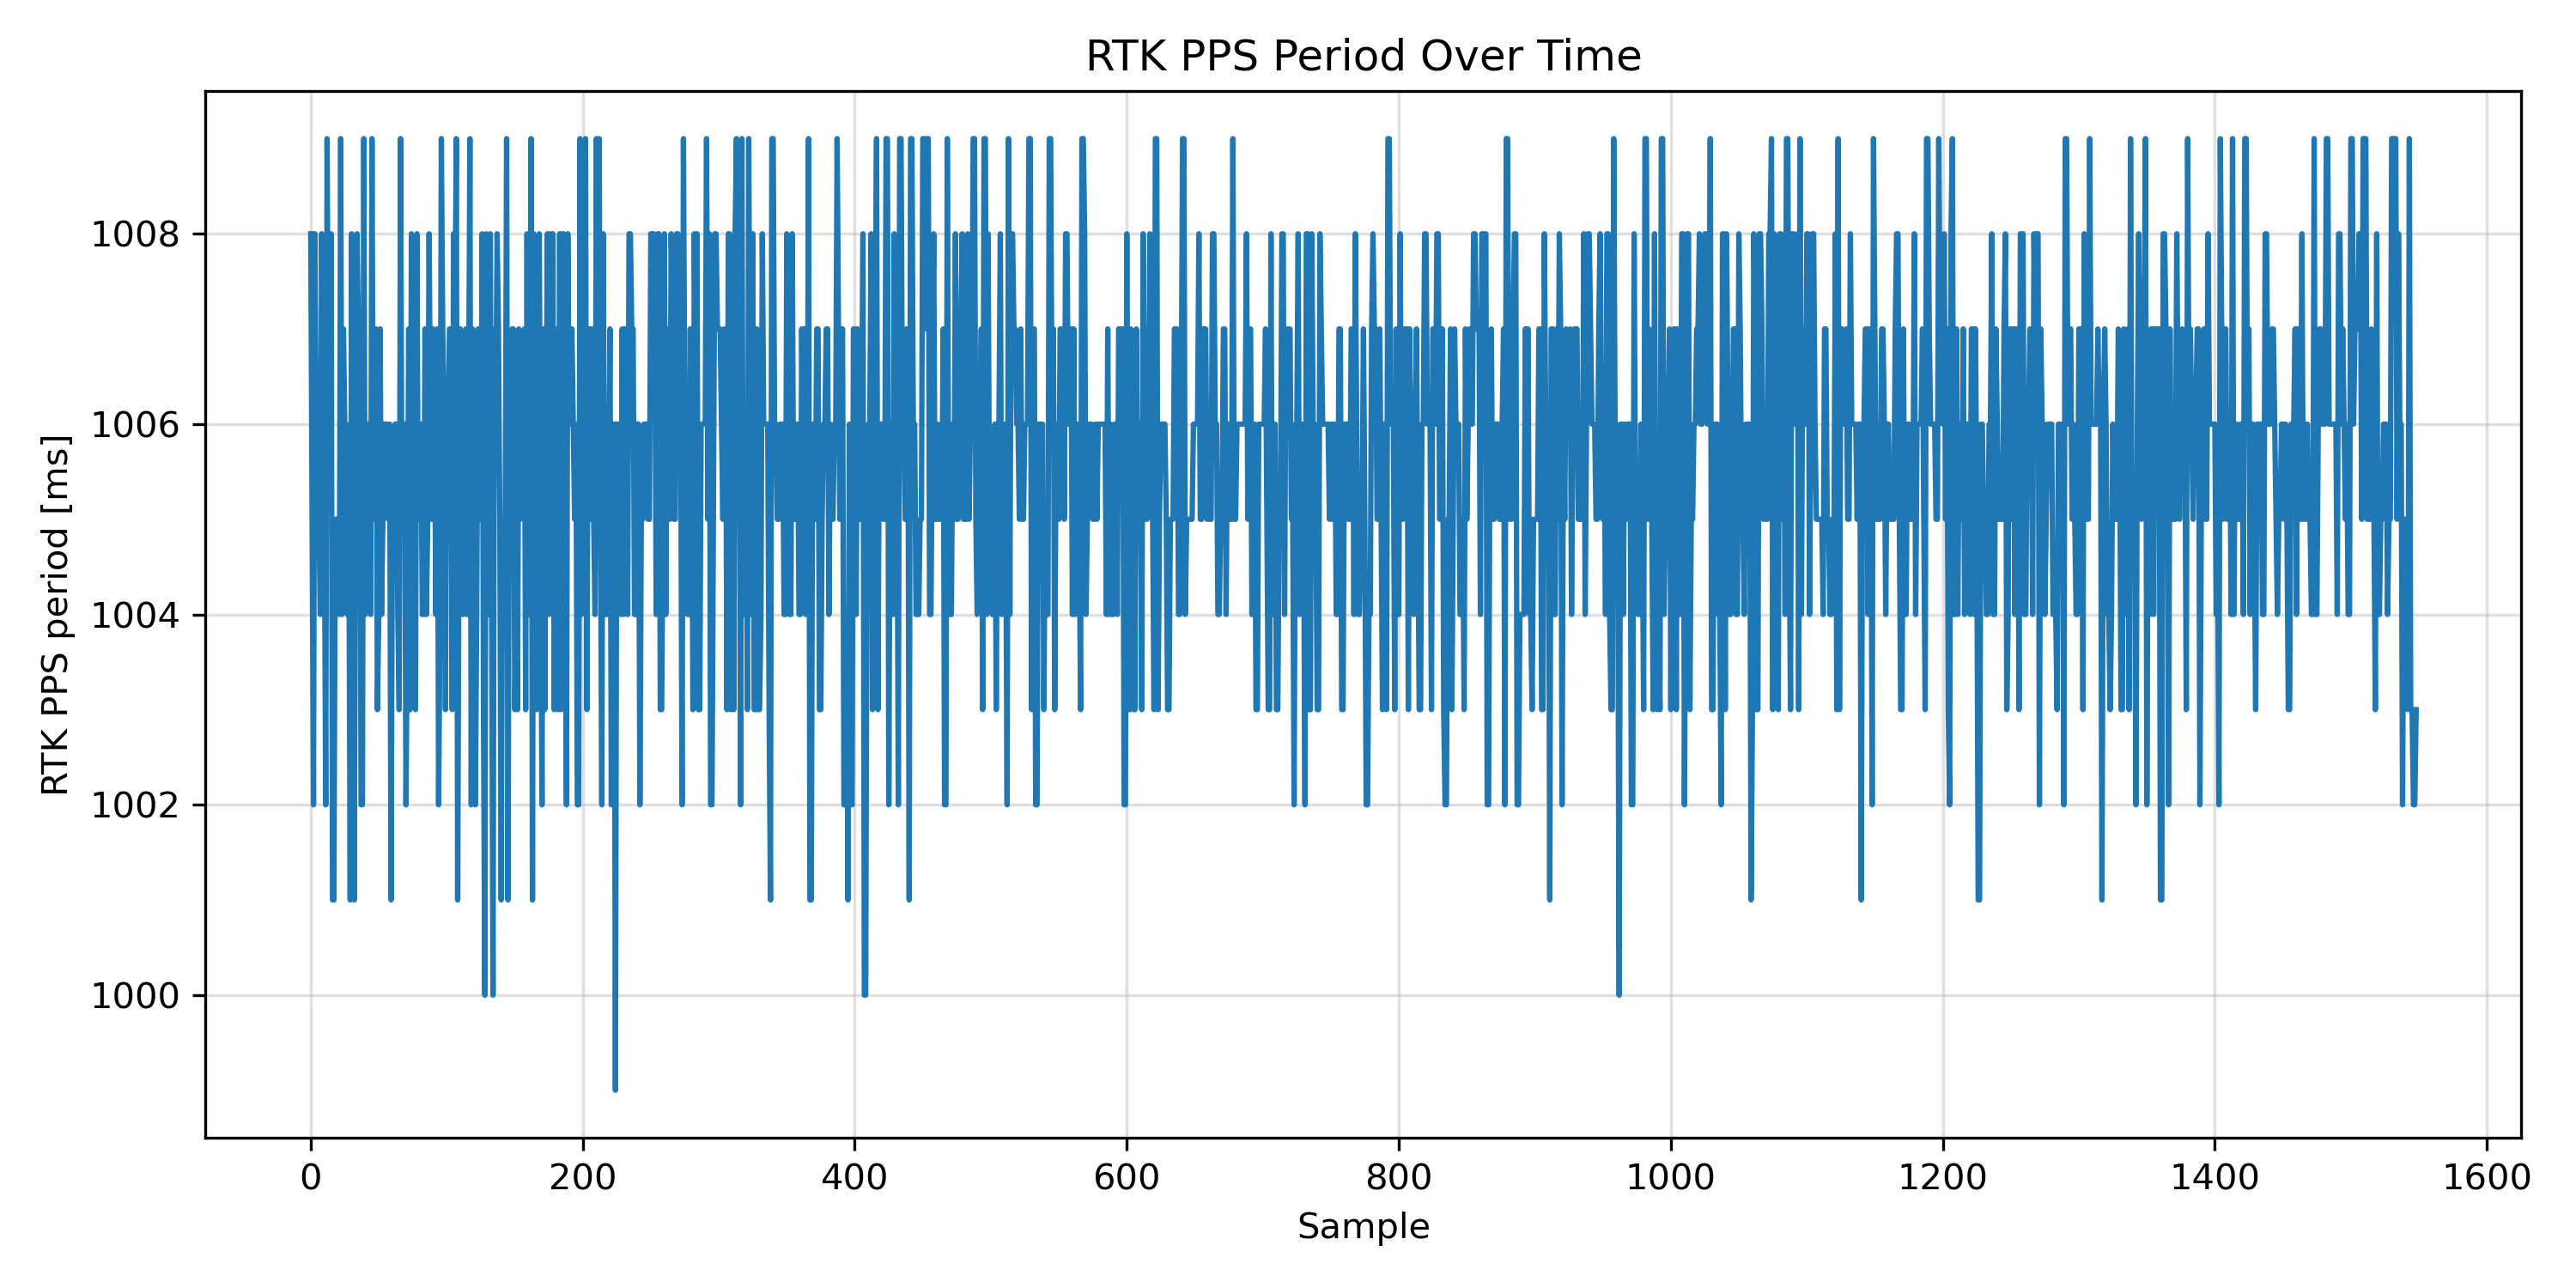
\includegraphics[width=1\textwidth]{fig/photos/final_rtk_delta.png}
  \caption{Measured RTK PPS period over time. The PPS period remained close to one second, with visible variation caused by millisecond-level firmware and logging resolution.}
  \label{fig:finalRtkDelta}
\end{figure}

\begin{figure}[H]
  \centering
  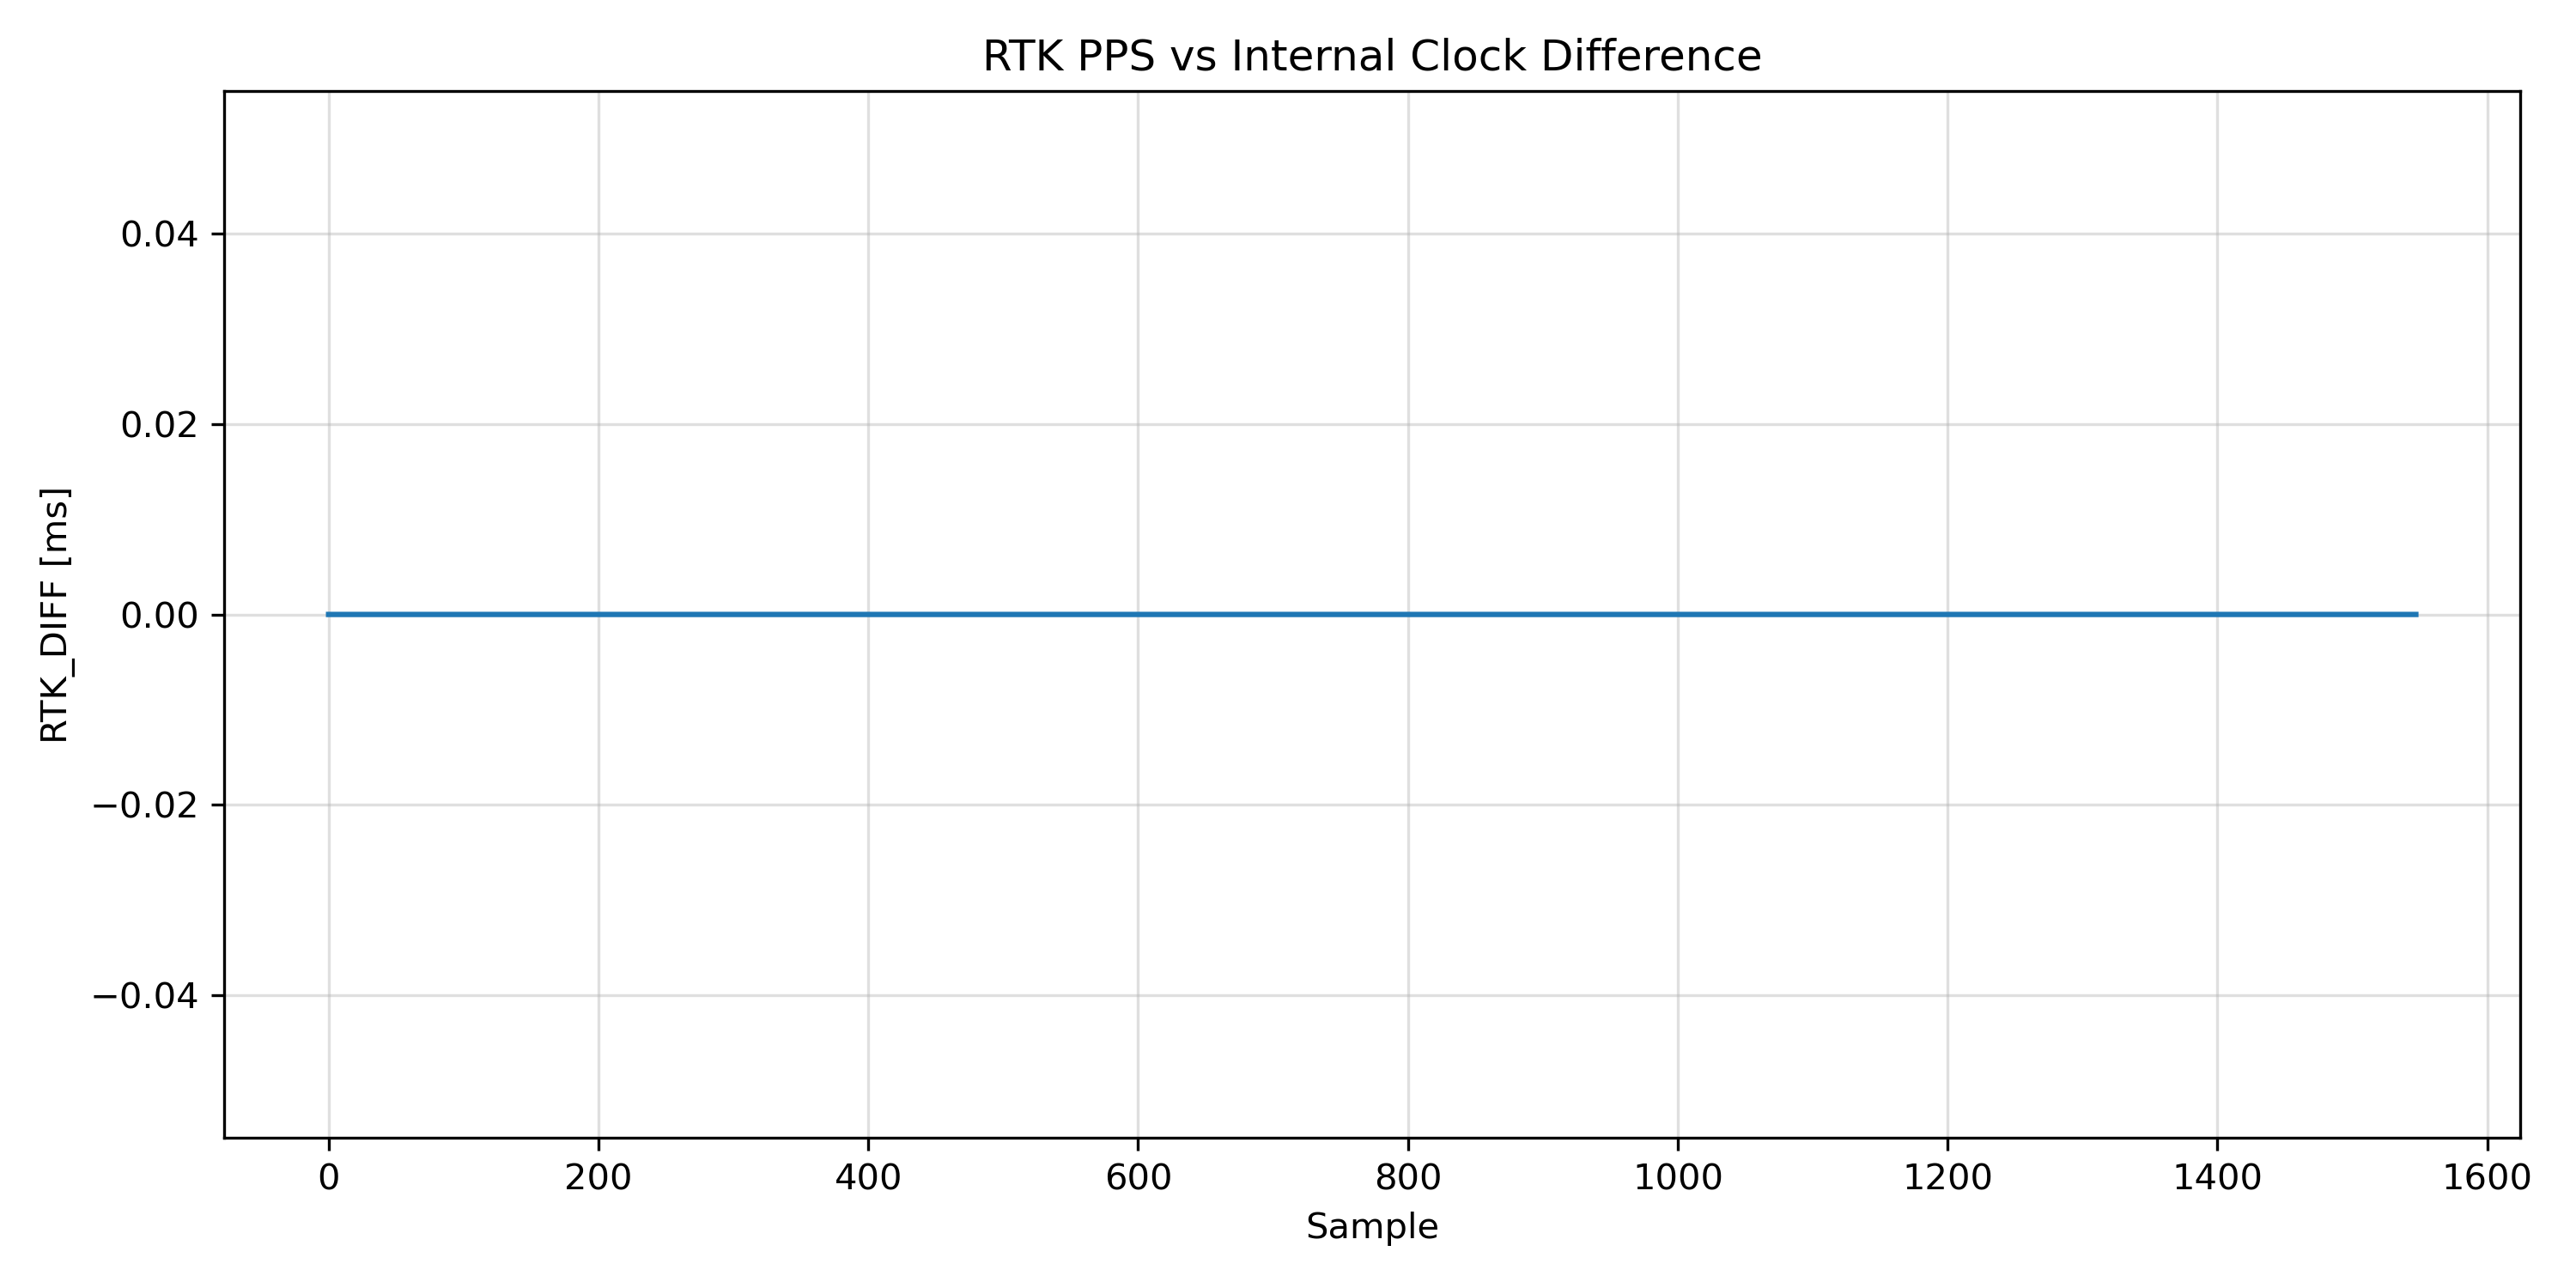
\includegraphics[width=1\textwidth]{fig/photos/final_rtk_diff.png}
  \caption{RTK PPS difference over time. The measured \texttt{RTK\_DIFF} remained equal to 0 ms during synchronized operation.}
  \label{fig:finalRtkDiff}
\end{figure}

\begin{figure}[H]
  \centering
  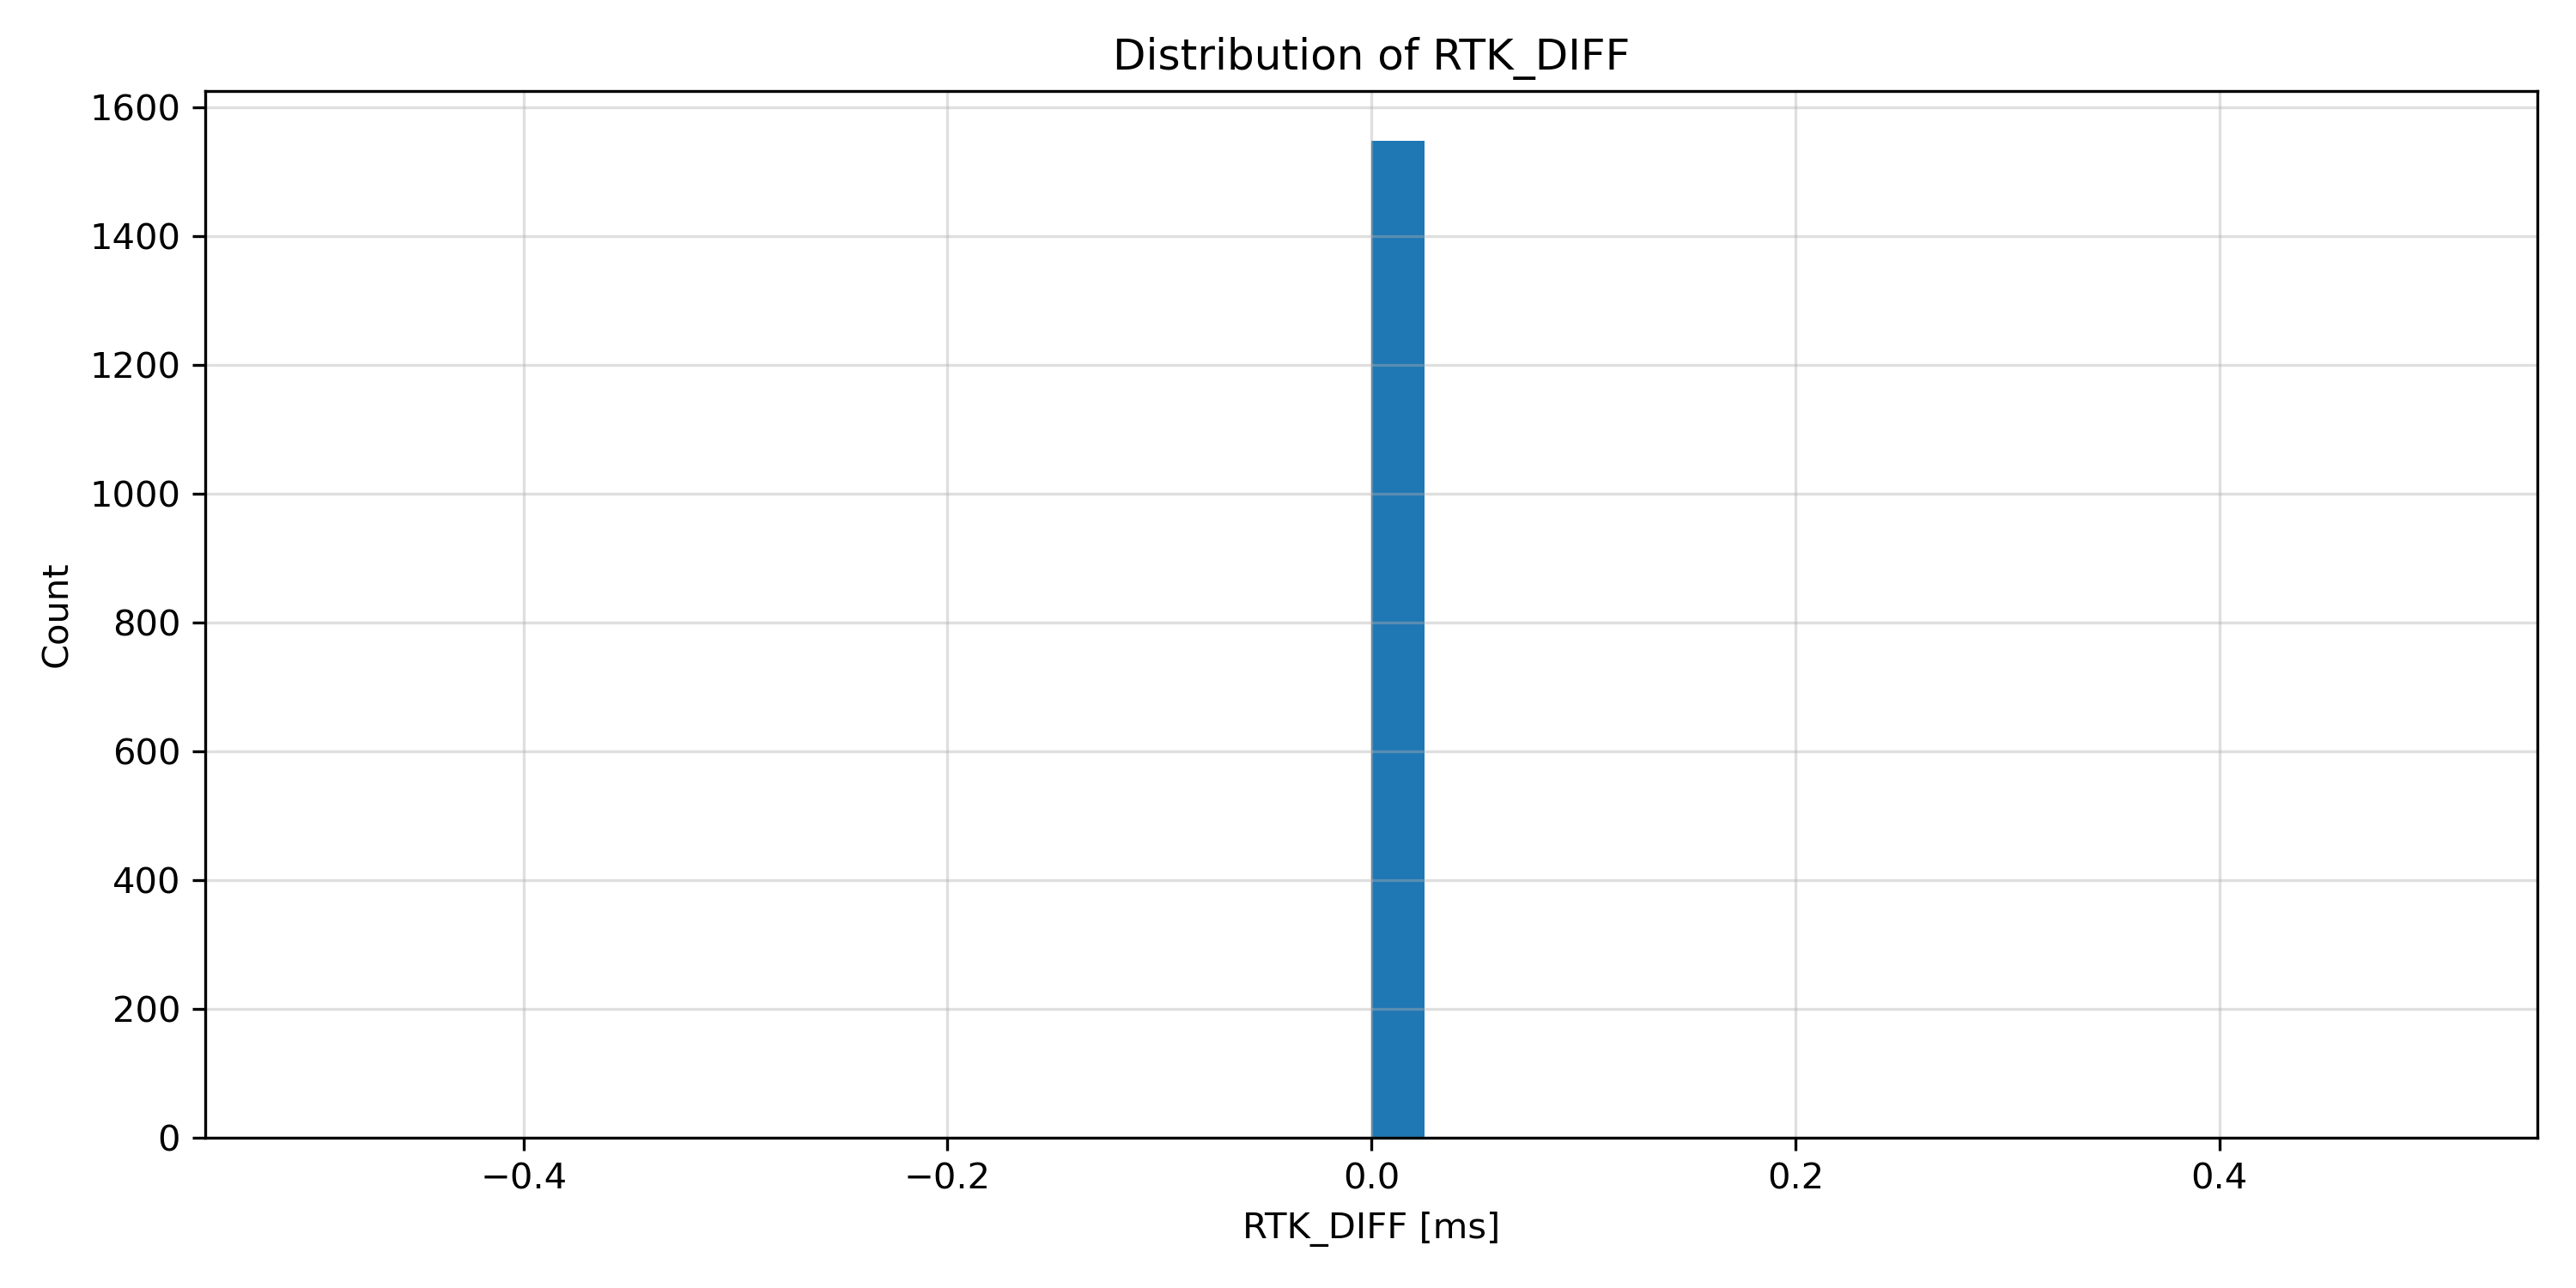
\includegraphics[width=1\textwidth]{fig/photos/final_rtk_diff_hist.png}
  \caption{Histogram of RTK PPS difference values. All synchronized samples were concentrated at 0 ms.}
  \label{fig:finalRtkDiffHist}
\end{figure}

\begin{figure}[H]
  \centering
  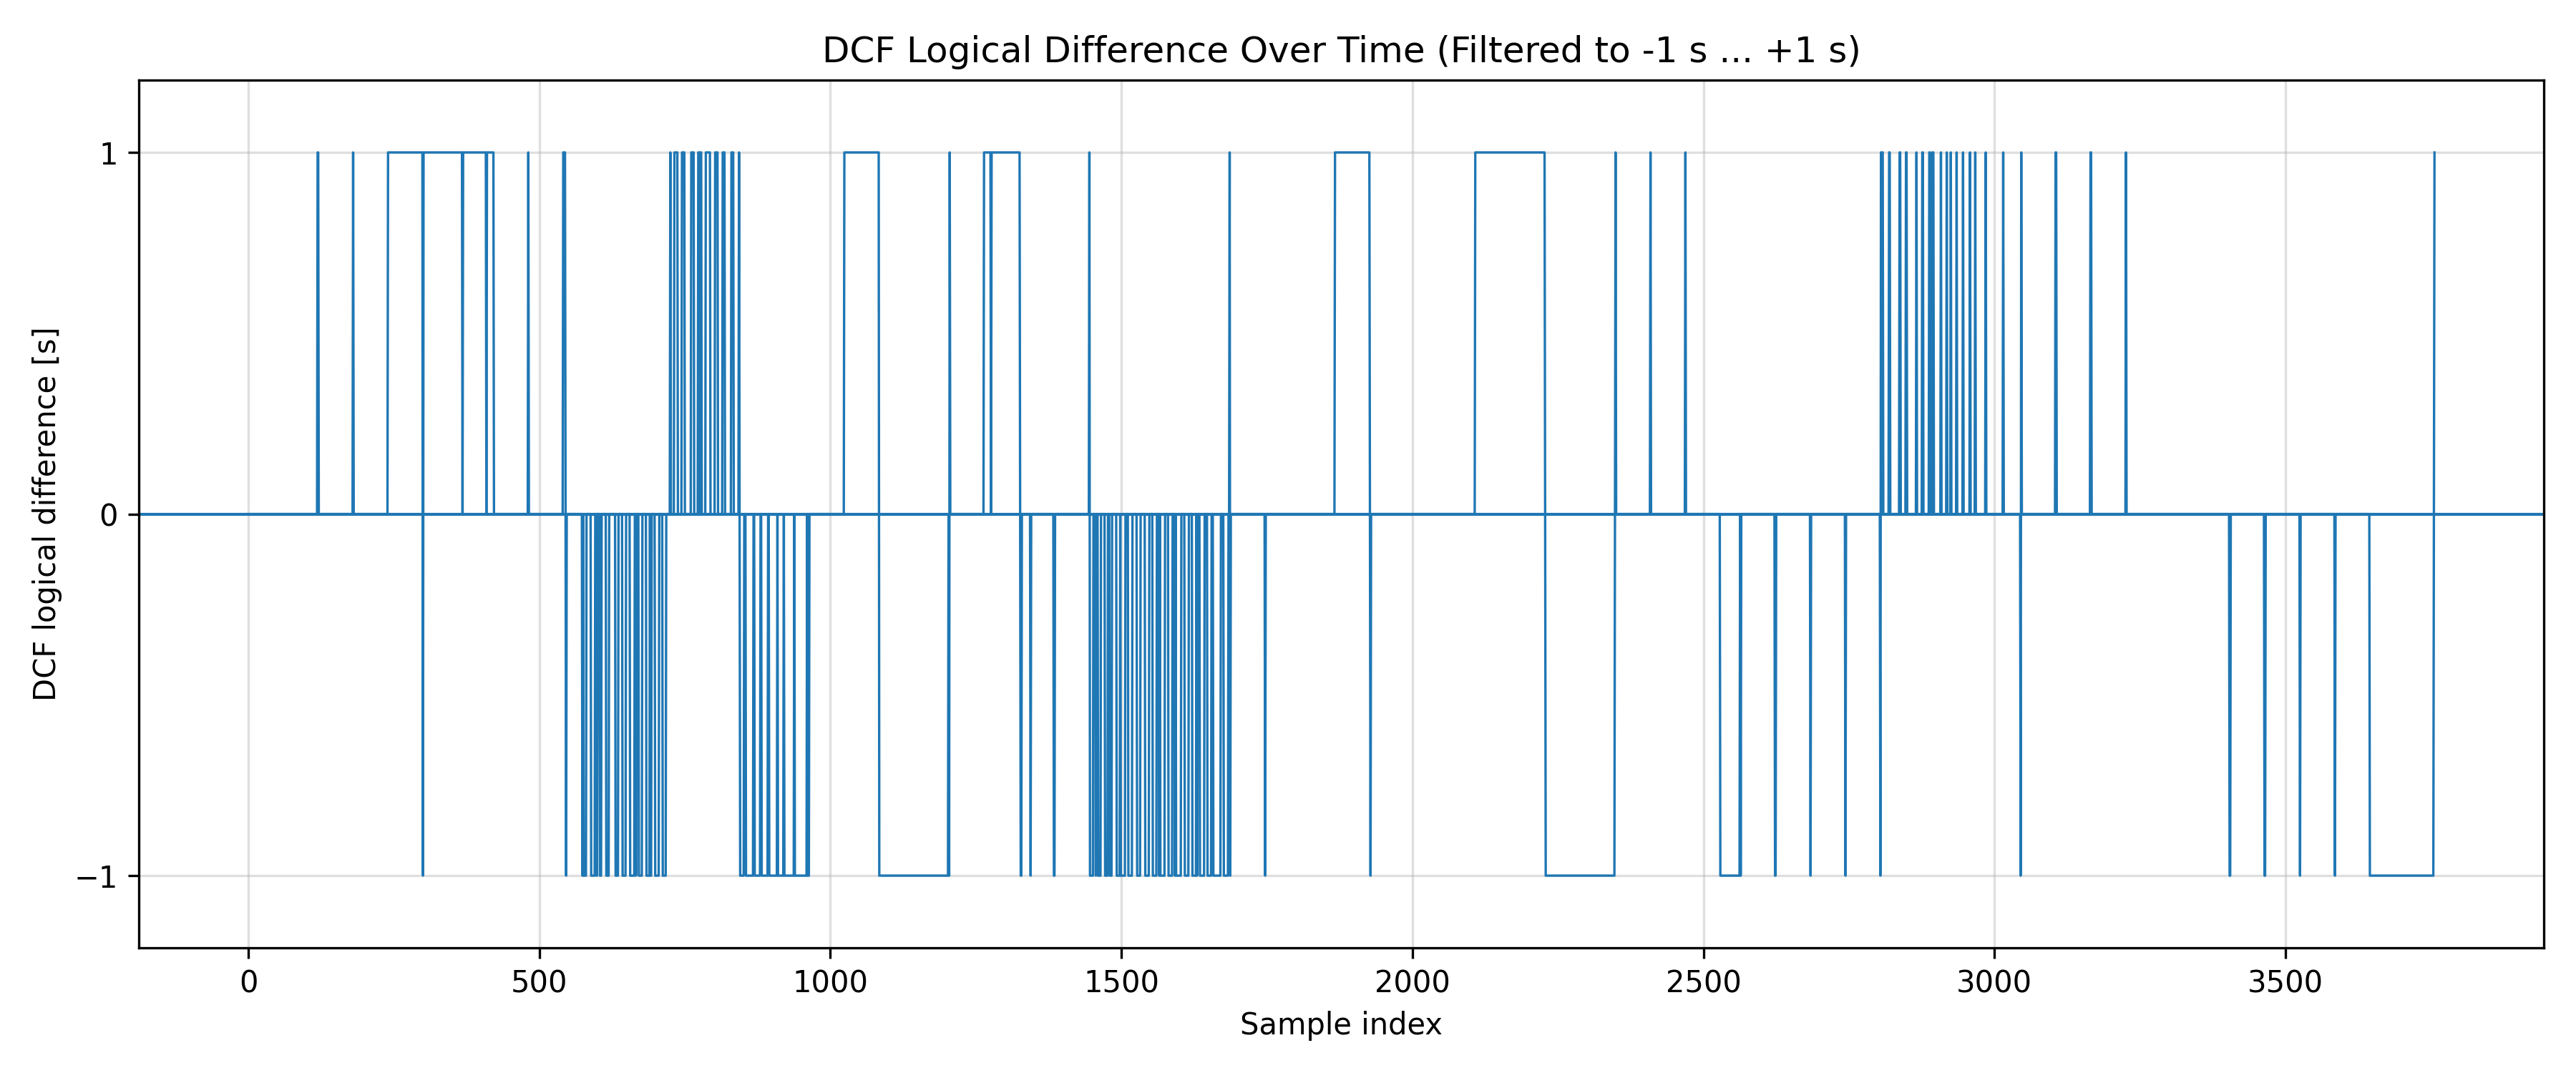
\includegraphics[width=1\textwidth]{fig/photos/DCF diff over time.png}
  \caption{Logical DCF77 time difference between two synchronization boards over time. Most samples remain close to zero, while temporary larger differences correspond to synchronization transitions or minute-boundary effects.}
  \label{fig:dcfDiffOverTime}
\end{figure}

\begin{figure}[H]
  \centering
  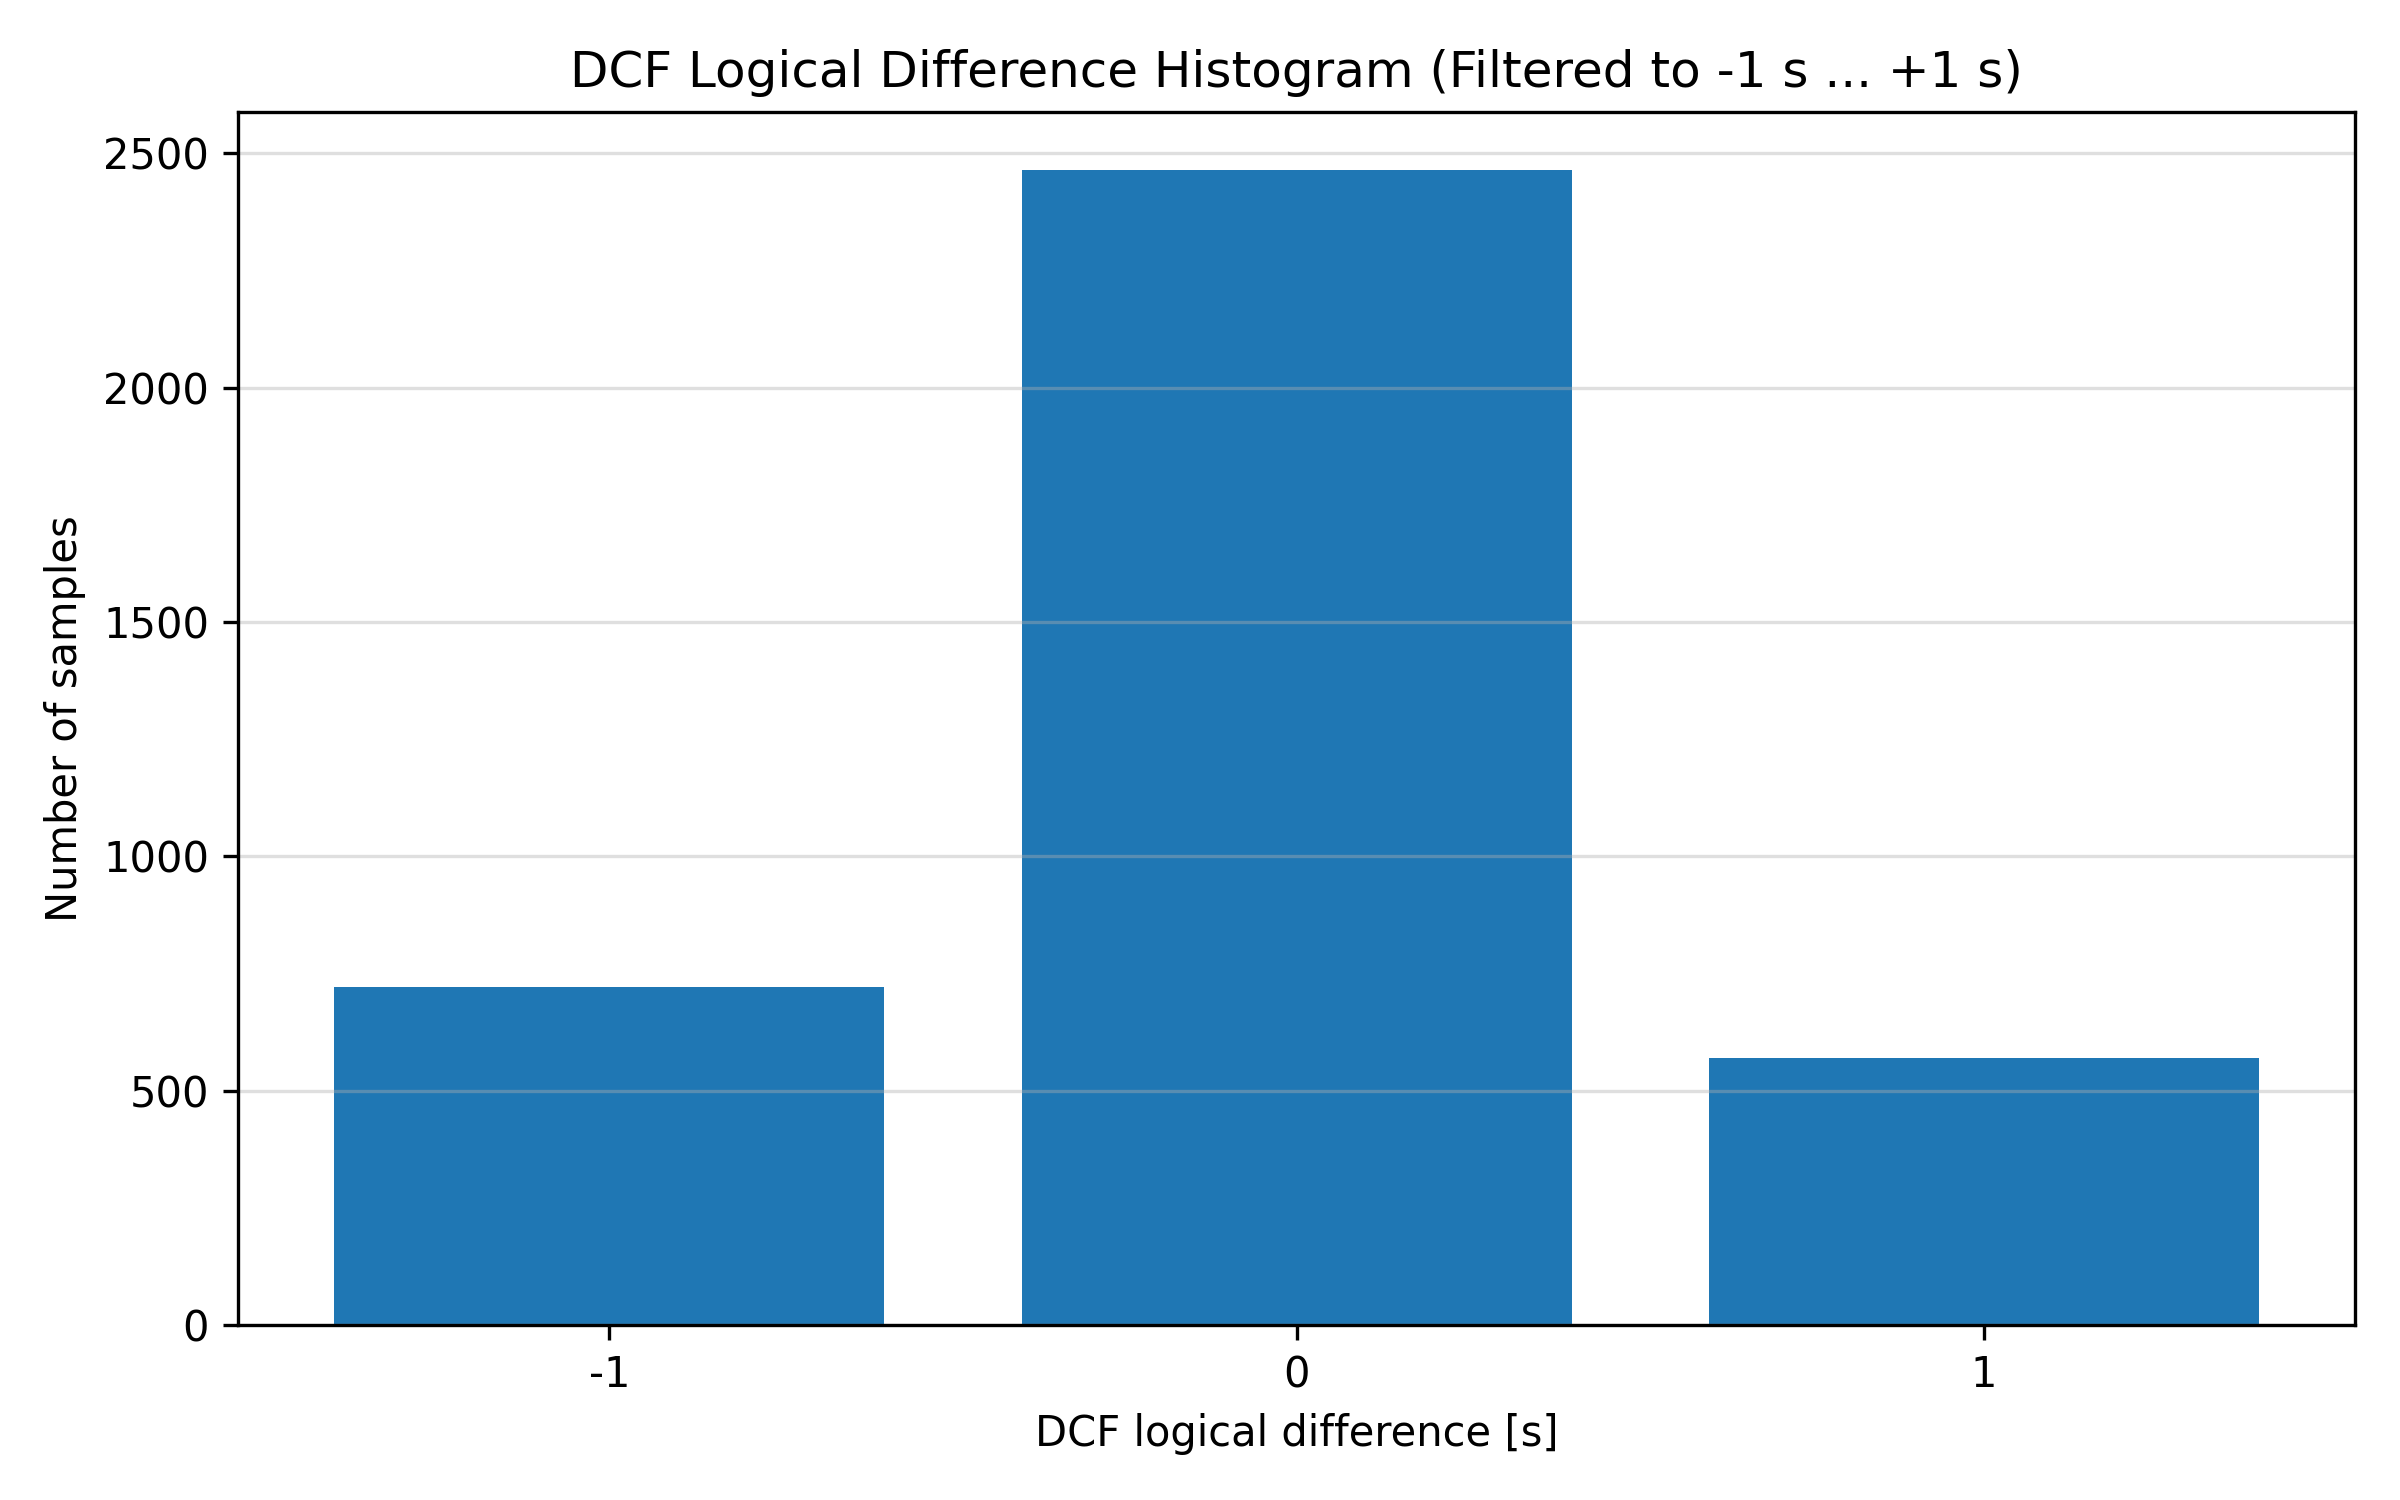
\includegraphics[width=1\textwidth]{fig/photos/DCF diff histogram.png}
  \caption{Histogram of logical DCF77 time differences between two synchronization boards. The distribution shows that most samples are concentrated near zero during stable operation.}
  \label{fig:dcfDiffHistogram}
\end{figure}

\begin{figure}[H]
  \centering
  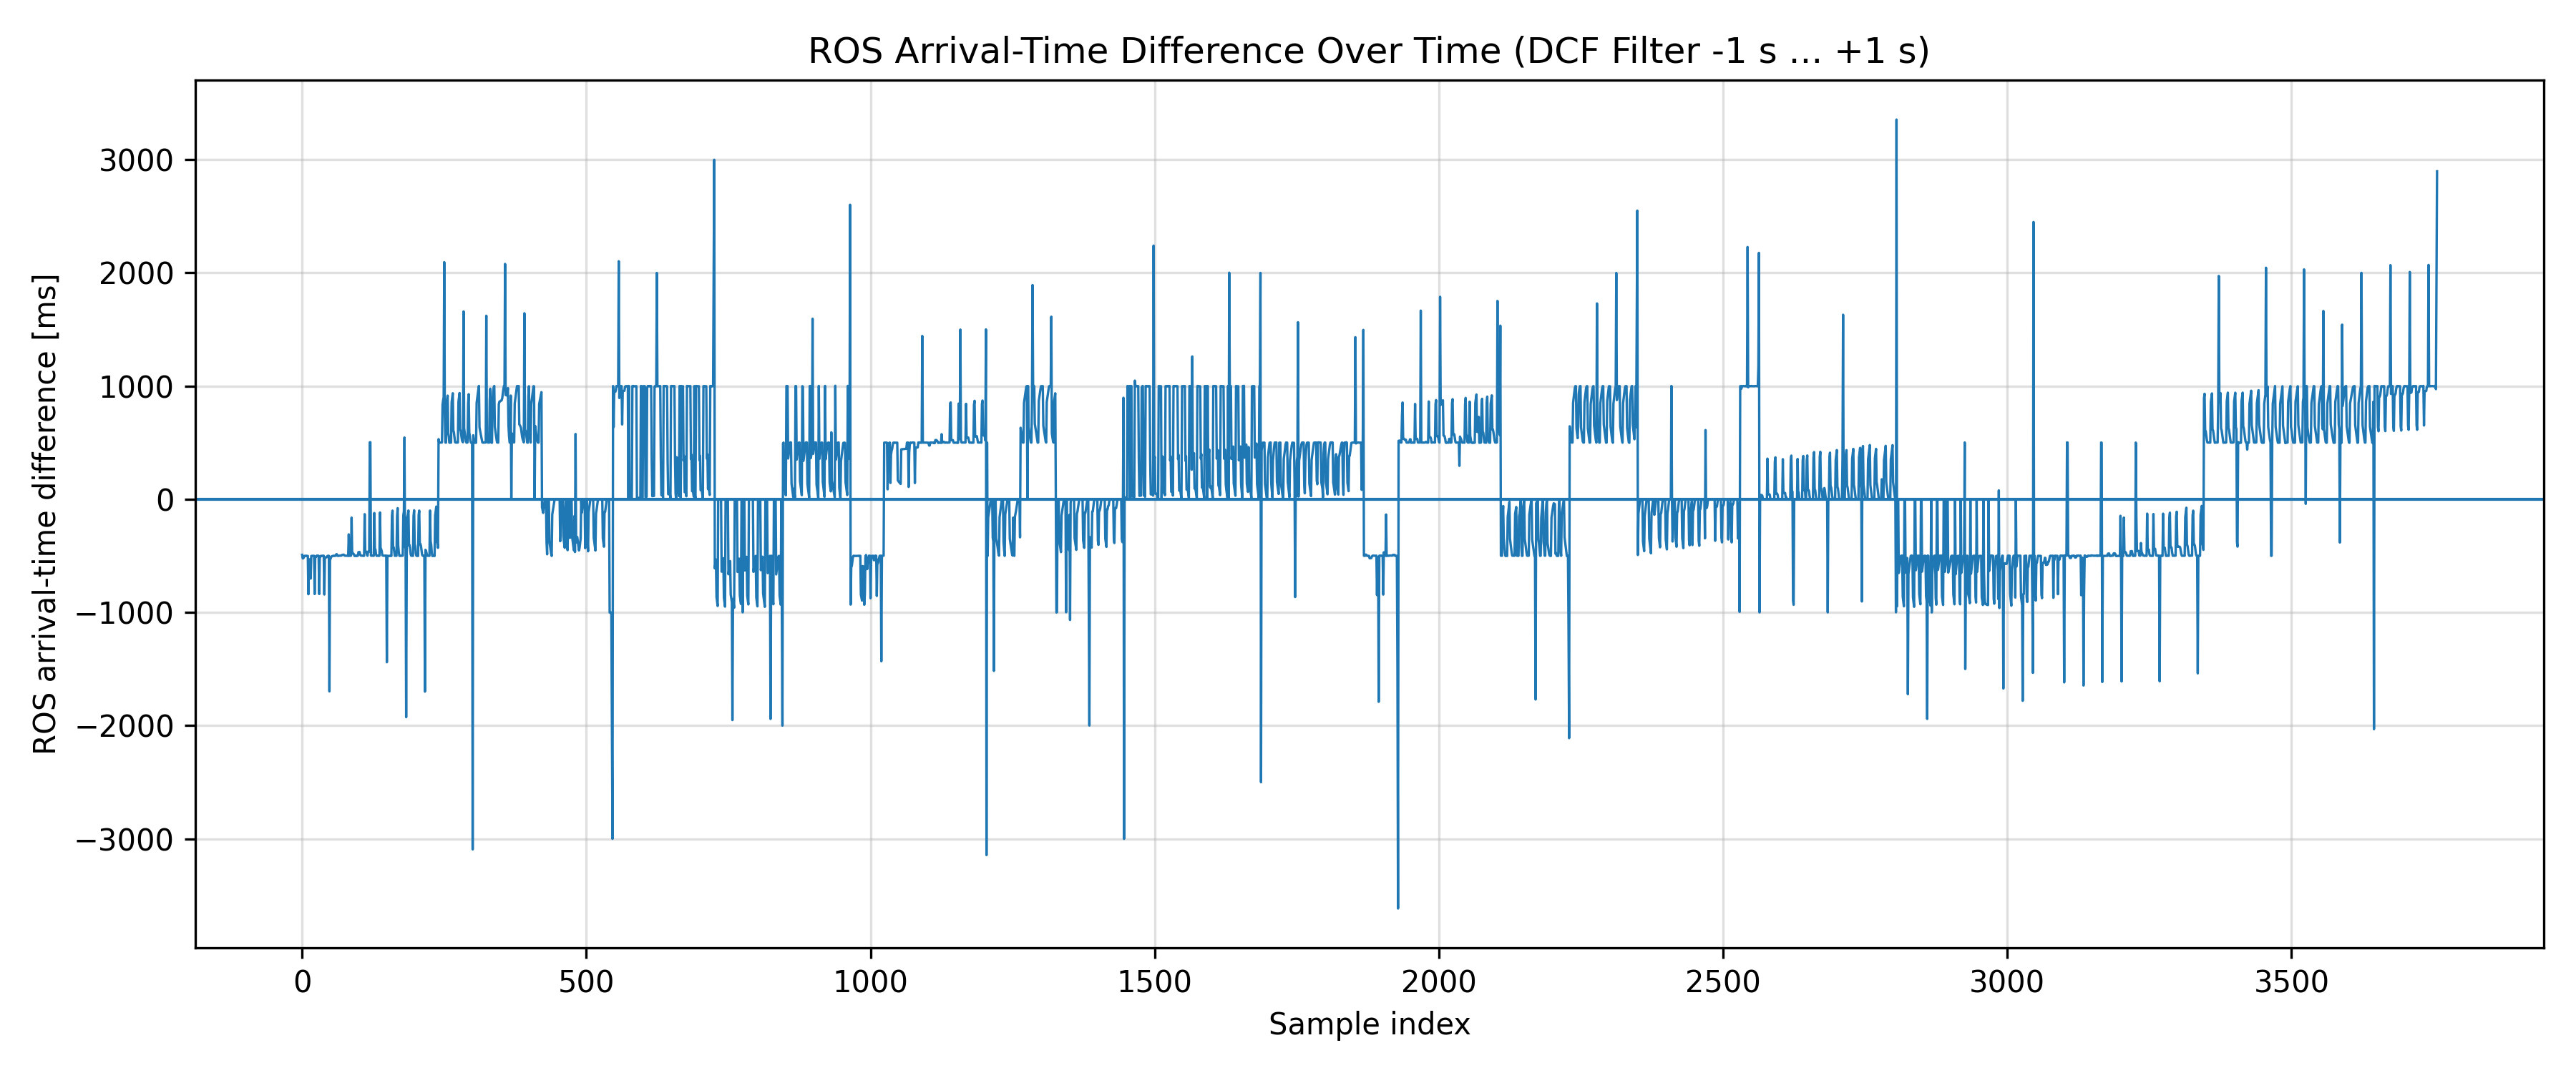
\includegraphics[width=1\textwidth]{fig/photos/ROS arrival diff over time.png}
  \caption{ROS2 arrival-time difference between two UART synchronization streams. The larger variations show communication and operating-system timing effects, not direct STM32 clock drift.}
  \label{fig:rosArrivalDiffOverTime}
\end{figure}

\section{CSV Log Format}
\label{app:csvLogFormat}

The ROS2 evaluation pipeline stored received synchronization messages in CSV files so that the data could be processed later by Python analysis scripts. Two main log files were used during testing: one for raw single-board UART messages and one for two-board comparison results.

The single-board serial log stored the ROS2 arrival timestamp together with the raw UART line received from the STM32 firmware. Its structure was:

\begin{verbatim}
ros_time_sec,ros_time_nsec,raw_line
\end{verbatim}

A typical row had the form:

\begin{verbatim}
1770000000,123456789,12:53:01 - 09.05.2026 - PCB_01 - SYNC=1
- LASTDCF=09.05.2026_12:53 - RTK_PPS=1543 - RTK_DELTA=1000ms
- RTK_DIFF=0ms
\end{verbatim}

The \texttt{raw\_line} field was parsed by the analysis script to extract synchronization state, RTK PPS period, and RTK difference values.

For two-board tests, the comparison node stored computed differences between the two received synchronization streams. The comparison CSV contained fields such as:

\begin{verbatim}
ros_time,dcf_diff_s,arrival_diff_ms,selected_source,selected_age
\end{verbatim}

The \texttt{dcf\_diff\_s} field represented the logical time difference between the two STM32 software clocks, while \texttt{arrival\_diff\_ms} represented the difference between ROS2 message arrival times. The first value was used to evaluate synchronization consistency between boards, while the second value was used to analyze the communication and logging pipeline.

This CSV-based format made the evaluation reproducible. The same logged files could be reprocessed to generate statistical summaries, RTK PPS plots, DCF77 comparison plots, and ROS2 arrival-time plots.

\end{document}
